\documentclass[11pt]{report}
\usepackage{amsfonts,amsthm,amsmath}
\usepackage[margin=1in]{geometry}
\usepackage{mathtools}
\usepackage{complexity}
\usepackage[chapter]{algorithm}
\usepackage{algpseudocode,caption} 
\usepackage{graphicx}
\usepackage{relsize}
\usepackage{tikz}  %TikZ central library is called.
\usepackage{tkz-graph}
\usepackage{tkz-berge}
%\usepackage{tikz-network}
\usetikzlibrary{automata,positioning,calc}
\usepackage[colorlinks=true,linkcolor=blue,citecolor=blue]{hyperref}

\usepackage{tocloft}
\usepackage{mathpazo}
\usepackage{xcolor}
\usepackage{color}
\definecolor{delta}{rgb}{0,0.2,0}
\definecolor{gamma}{rgb}{0,0,0.2}
\definecolor{beta}{rgb}{0.2,0,0}
\definecolor{alpha}{rgb}{0.8,0,0}
\newcommand{\wt}[1]{\widetilde{#1}}
\newcommand{\sse}{\subseteq}
\newcommand{\zo}{\{0,1\}}
\newcommand{\zon}{\zo^n}
\newcommand{\aphantom}{\vphantom{2^2}}
\newcommand{\aaphantom}{\vphantom{2^{2^2}}}
\newcommand{\defn}{\stackrel{\text{\tiny def}}{=}}

% left-right wrappers
\newcommand{\set}[1]{\left\{ #1 \right\}}
\newcommand{\card}[1]{\left|#1 \right|}
\newcommand{\mytilde}[1]{\overset{\sim}{#1}}

% latin
\newcommand{\etal}{\textit{et al}.\@\xspace}
\newcommand{\ie}{i.e.}
\usepackage[all]{xy}
\usepackage{setspace}
\usepackage{amssymb}
\usepackage{amsmath}
\newtheoremstyle{myplain}{10pt}{10pt}{\itshape}{}{\scshape}{.}{.5em}{}
\newtheoremstyle{mydefinition} {10pt}{10pt}{\itshape}{}{\scshape}{.}{.5em}{}
\newtheoremstyle{myremark}     {10pt}{10pt}{}{}{\scshape}{.}{.5em}{}
\newcounter{week}
\theoremstyle{myplain}

\newtheorem{theorem}{Theorem}[section]
\newtheorem{lemma}         [theorem]{Lemma}
\newtheorem{proposition}   [theorem]{Proposition}
\newtheorem{corollary}     [theorem]{Corollary}
\newtheorem{claim}         [theorem]{Claim}
\newtheorem{fact}          [theorem]{Fact}
\theoremstyle{mydefinition}
\newtheorem{definition}    [theorem]{Definition}
\newtheorem{example}       [theorem]{Example}
\newtheorem{assumption}    [theorem]{Assumption}
\newtheorem{openproblem}   [theorem]{Open Problem}
\newtheorem{problem}       [theorem]{Problem}
\theoremstyle{myremark}
\newtheorem{remark}        [theorem]{Remark}
\newtheorem{conjecture}    [theorem]{Conjecture}
\numberwithin{equation} {week}
\numberwithin{figure}   {week}
\numberwithin{table}    {week}
\newcommand{\cupdot}{\mathbin{\mathaccent\cdot\cup}}
\newcommand{\bigsum}{\mathlarger{\mathlarger{\sum}}}
\newcommand{\bigger}[1]{\mathlarger{\mathlarger{#1}}}
\renewcommand{\bar}[1]{\overline{\vphantom{1^a}#1}}
%\renewcommand{\fnum@figure}{\textsc{Figure~\thefigure}}
%\renewcommand{\fnum@table}{\textsc{Table~\thetable}}

\AtBeginDocument{\renewcommand\contentsname{Table of Contents}}
\newcommand{\listofscribes}{List of Scribes}
\newlistof{scribe}{scr}{\listofscribes}

\newcommand{\Week}[2]
{
	\setcounter{chapter}{#1}
	\setcounter{section}{0}
	\setcounter{week}{#1}
	% For table of contents
	\addcontentsline{toc}{chapter}{\protect	\numberline{#1}{Week #1 : #2}}
	% For list of scribes
	%	\addcontentsline{scr}{scribe}{\protect {\sf Lecture 	} \numberline{\sf \thelecture} {\em #1}}

	\noindent
	\newpage
	\parbox{12cm}{
		{\Large \sf #2} \\[5mm]
		{\large Lecturer : Jayalal Sarma}\\
	}
	\hfill
	\begin{tabular}{c@{}}
	{\bf\Large WEEK}\\[2mm]
	\rule{0mm}{17mm}\scalebox{7}{\bf\theweek}
	\end{tabular}
	\vspace{1cm}
	\hrule
	\vspace{1cm}
}

\newtheorem{observation}[theorem]{Observation}
%\newtheorem{exercise}{Exercise}
\theoremstyle{plain}

\newenvironment{proof-sketch}{\noindent{\bf Sketch of Proof}\hspace*{1em}}{\qed\bigskip}
\newenvironment{proof-idea}{\noindent{\bf Proof Idea}\hspace*{1em}}{\qed\bigskip}
\newenvironment{proof-of-lemma}[1]{\noindent{\bf Proof of Lemma #1}\hspace*{1em}}{\qed\bigskip}
\newenvironment{proof-attempt}{\noindent{\bf Proof Attempt}\hspace*{1em}}{\qed\bigskip}
\newenvironment{proofof}[1]{\noindent{\bf Proof}
of #1:\hspace*{1em}}{\qed\bigskip}

\renewcommand{\qedsymbol}{\leavevmode
  \hbox to.77778em{%
  \hfil\vrule
  \vbox to.875em{\hrule width.35em\vfil\hrule}%
  \vrule\hfil}}

%%%%%%%%%%%%%%%%%%%%%%%%%%%%%%%%%%%%%%%%%%%%%%%%%%%
% Useful Macros
%%%%%%%%%%%%%%%%%%%%%%%%%%%%%%%%%%%%%%%%%%%%%%%%%%%
\newcommand{\Exp}[1]{\mathify{\mbox{Exp}\left[#1\right]}}
\newcommand{\bigO}O
%\newcommand{\set}[1]{\mathify{\left\{ #1 \right\}}}
\def\half{\frac{1}{2}}
\newcommand{\V}[1]{\mathsf{Var}[#1]}
\def\implies{\Rightarrow}
\def\prob#1#2{{\mathop{{\rm Prob}}_{#1}}\left[#2 \right]}
\def\var#1#2{{\mathop{{\rm Var}}_{#1}}[#2]}
\def\expec#1#2{{\mathop{{\rm E}}_{#1}}[#2]}
\def\sizeof#1{\left| #1\right|}
\def\setof#1{\left\{ #1\right\}  }
\newcommand\norm[1]{{\left\lVert#1\right\rVert}_2}
\newcommand{\F}{{\mathbb{F}}}
\newcommand{\Z}{{\mathbb{Z}}}
\newcommand{\supp}{{\mathsf{supp}}}
%\newcommand{\qed}{\rule{7pt}{7pt}}
\newcommand*\circled[1]{~\tikz[baseline=(char.base)]{
            \node[shape=circle,draw,inner sep=1.5pt] (char) {\tiny #1};}~}
        
% \makeatletter
% \@addtoreset{figure}{section}
% \@addtoreset{table}{section}
% \@addtoreset{equation}{section}
% \makeatother

\newcommand{\FOR}{{\bf for}}
\newcommand{\TO}{{\bf to}}
\newcommand{\DO}{{\bf do}}
\newcommand{\WHILE}{{\bf while}}
\newcommand{\AND}{{\bf and}}
\newcommand{\IF}{{\bf if}}
\newcommand{\THEN}{{\bf then}}
\newcommand{\ELSE}{{\bf else}}
\newcommand{\N}{\mathbb{N}}

% \renewcommand{\thefigure}{\thesection.\arabic{figure}}
% \renewcommand{\thetable}{\thesection.\arabic{table}}
% \renewcommand{\theequation}{\thesection.\arabic{equation}}

% Calligraphic letters
\newcommand{\calA}{{\cal A}}
\newcommand{\calB}{{\cal B}}
\newcommand{\calC}{{\cal C}}
\newcommand{\calD}{{\cal D}}
\newcommand{\calE}{{\cal E}}
\newcommand{\calF}{{\cal F}}
\newcommand{\calG}{{\cal G}}
\newcommand{\calH}{{\cal H}}
\newcommand{\calI}{{\cal I}}
\newcommand{\calJ}{{\cal J}}
\newcommand{\calK}{{\cal K}}
\newcommand{\calL}{{\cal L}}
\newcommand{\calM}{{\cal M}}
\newcommand{\calN}{{\cal N}}
\newcommand{\calO}{{\cal O}}
\newcommand{\calP}{{\cal P}}
\newcommand{\calQ}{{\cal Q}}
\newcommand{\calR}{{\cal R}}
\newcommand{\calS}{{\cal S}}
\newcommand{\calT}{{\cal T}}
\newcommand{\calU}{{\cal U}}
\newcommand{\calV}{{\cal V}}
\newcommand{\calW}{{\cal W}}
\newcommand{\calX}{{\cal X}}
\newcommand{\calY}{{\cal Y}}
\newcommand{\calZ}{{\cal Z}}


\setcounter{tocdepth}{3}
\setcounter{secnumdepth}{2}
\sloppy

\newcommand{\AsymCloud}[3]{
\begin{scope}[shift={#1},scale=#3]
\draw (-1.6,-0.7) .. controls (-2.3,-1.1)
and (-2.7,0.3) .. (-1.7,0.3)coordinate(asy1) .. controls (-1.6,0.7)
and (-1.2,0.9) .. (-0.8,0.7) .. controls (-0.5,1.5)
and (0.6,1.3) .. (0.7,0.5) .. controls (1.5,0.4)
and (1.2,-1) .. (0.4,-0.6)coordinate(asy2) .. controls (0.2,-1)
and (-0.2,-1) .. (-0.5,-0.7) .. controls (-0.9,-1)
and (-1.3,-1) .. cycle;
\node at ($(asy1)!0.5!(asy2)$) {#2};
\end{scope}
}
\usepackage{collect}
\usepackage{hypcap}
\renewcommand{\E}{{\mathbb E}}

\usepackage{todonotes}
\newcounter{todocounter}
\newcommand{\todonum}[2][]{\stepcounter{todocounter}\todo[#1]{\thetodocounter: #2}}
\newcommand{\jsay}[1]{\todonum[inline,color=red!20]{\small Jayalal says: Todo - #1}}

% modified exercise enviornment to use with collect  package
\usepackage{enumerate}
\newcounter{excount}
\setcounter{excount}{0}
\theoremstyle{definition}
\newtheorem{ex}[theorem]{Exercise}
\newtheorem{curious}[theorem]{Curiosity}
% for exercises which are problem set questions

\newtheorem{exercise-prob}[theorem]{Exercise}
\theoremstyle{plain}	    
%%%%%%%%%%%%%%%%%%%% Exercise and pset macros (start) %%%%%%%%%%%%%%%%%%%%%%%5
% For problem set back reference.
\def\psetbackref{1}

% For Curiosity Drive
\definecollection{curious.tmp}
\makeatletter
\newenvironment{curiousity}
    {\@nameuse{collect*}{curious.tmp}
		  {\begin{curious}}
		    {\end{curious}}{}{}
    }{\@nameuse{endcollect*}}
\makeatother

% For exercise
\definecollection{ex.tmp}
\makeatletter
\newenvironment{exercise}
    {\@nameuse{collect*}{ex.tmp}
		  {\begin{ex}}
		    {\end{ex}}{}{}
    }{\@nameuse{endcollect*}}
\makeatother


%%%%%%%%%%%%%%%%%%%%%%%%%%%%%%%%%%%%%%%%%%%%%%%%%%%%%%%%%%%%%%
% To create a a new pset with pset number n, copy paste the following code
% with XX replaced by n.
%
% 	 \definecollection{psXX.tmp}
%	 \makeatletter
%	 \newenvironment{show-psXX}[1]
%	     {\@nameuse{collect*}{psXX.tmp}
%	         {\ifthenelse{ \equal{\psetbackref}{1} }{\label{prob:#1}}{}} {}
%   	         {\item \label{#1} (See Exercise~\ref{prob:#1})} {}
%	     }{\@nameuse{endcollect*}}
%	 \makeatother
%
%	 \makeatletter
%	 \newenvironment{psXX}
%	     {\@nameuse{collect}{psXX.tmp}
%			{\item}{}
%	     }{\@nameuse{endcollect}}
%	 \makeatother
%
% 

%%% For ps1 
\definecollection{ps1.tmp}
\makeatletter
\newenvironment{show-ps1}[1]
    {\@nameuse{collect*}{ps1.tmp}
	    {\ifthenelse{ \equal{\psetbackref}{1} }			{\label{prob:#1}}{}} {}
	    {\item \label{#1} (See Exercise~\ref{prob:#1})} {}
    }{\@nameuse{endcollect*}}
\makeatother

\makeatletter
\newenvironment{ps1}
    {\@nameuse{collect}{ps1.tmp}
		{\item }{}
    }{\@nameuse{endcollect}}
\makeatother

%%% For ps2
\definecollection{ps2.tmp}
\makeatletter
\newenvironment{show-ps2}[1]
    {\@nameuse{collect*}{ps2.tmp}
	    {\ifthenelse{ \equal{\psetbackref}{1} }{\label{prob:#1}}{}} {}
	    {\item \label{#1} (See Exercise~\ref{prob:#1})} {}
    }{\@nameuse{endcollect*}}
\makeatother

\makeatletter
\newenvironment{ps2}
    {\@nameuse{collect}{ps2.tmp}
		{\item}{}
    }{\@nameuse{endcollect}}
\makeatother

%%% For ps3
\definecollection{ps3.tmp}
\makeatletter
\newenvironment{show-ps3}[1]
    {\@nameuse{collect*}{ps3.tmp}
	    {\ifthenelse{ \equal{\psetbackref}{1} }{\label{prob:#1}}{}} {}
	    {\item \label{#1} (See Exercise~\ref{prob:#1})} {}
    }{\@nameuse{endcollect*}}
\makeatother

\makeatletter
\newenvironment{ps3}
    {\@nameuse{collect}{ps3.tmp}
		{\item}{}
    }{\@nameuse{endcollect}}
\makeatother


%%% For ps3
\definecollection{ps4.tmp}
\makeatletter
\newenvironment{show-ps4}[1]
    {\@nameuse{collect*}{ps4.tmp}
	    {\ifthenelse{ \equal{\psetbackref}{1} }{\label{prob:#1}}{}} {}
	    {\item \label{#1} (See Exercise~\ref{prob:#1})} {}
    }{\@nameuse{endcollect*}}
\makeatother

\makeatletter
\newenvironment{ps4}
    {\@nameuse{collect}{ps4.tmp}
		{\item}{}
    }{\@nameuse{endcollect}}
\makeatother

%%%%% Exercise and pset macros (end) %%%%%

\renewcommand{\E}{{\mathbb E}}
\title{{\huge \sf Course on Pseudorandomness} \\[3mm]
{\sf \LARGE(Lecture Notes)}\\[1cm]}
\author{{\Large {\sc Jayalal Sarma}} \\[3mm]
Department of Computer Science and Engineering \\[1mm]
Indian Institute of Technology Madras (IITM)\\[1mm]
Chennai, India}
\date{Last updated on : \today}
\begin{document}
\maketitle
\setcounter{page}{1}
\newpage
%\listofscribe
\setstretch{1.1}
\tableofcontents
\listoftodos
\setcounter{page}{1}
\part{General Introduction and Tools}
\Week{1}{Power of Randomization and Derandomization Problem}
\noindent 

Randomized algorithms play a very powerful role in algorithm design. We will concentrate on the randomized algorithms for decision problems in this course. So all of our computational problems can be abstractly represented as given a string $x \in \Sigma^*$ in an alphabet, does $x$ have property $\calP$ or not?

Informally, a randomized algorithm running in time $t$ is an algorithm that that on input $x$ is allowed to perform at most $t$ instances of random experiment of tossing unbiased coins during its computation and uses the outcome of the experiment in the computation, but however, provides a guarantee that the answer of the algorithm is the \textit{correct} answer for the input $x$ in a good fraction of the possible outcomes of the experiment. \footnote{Notice that if the guarantee for the algorithm is not saying "{\em strictly more than half fraction of the coin tosses}", then essentially the algorithm is useless since we can always replace it with a random experiment of tossing an unbiased coin and returning the answer to be {\sc Yes} if we get the heads and {\sc No} if we get tails. Note that we have at least a $\frac{1}{2}$ probability of success $\half$.}


\section{Randomness helps in Matrix Multiplication Verification}

Consider the task of multiplying two $n \times n$ matrices over the field $\F_2$. The trivial algorithmic solution to the problem takes $O(n^3)$ time and the trivial lower bound for the problem is $\Omega(n^2)$. It has been a long standing question which is the right complexity bound for this important problem (improvement to which will lead to improvements even in practice !). The exponent of matrix multiplication is the smallest constant $\omega$ such that two $n \times n$ matrices may be multiplied by performing $O(n^{\omega+\epsilon})$ for every $\epsilon > 0$.

Indeed, one of the basic ideas that we learn in algorithms courses for demonstrating the power of divide and conquer is the Strassen's multiplication which gives a running time bound of $O(n^{2.,73})$ which went through a sequence of improvements and to the current best of $O(n^{2.31})$.

The question that we address now is something closely related - that of verifying whether a given multiplicaiton is correct.
\begin{problem}
Given three matrices $A,B, C \in \F_2^{n \times n}$, check whether $AB = C$ or not.
\end{problem}

Indeed, the trivial method would be to mutliply the two matrices and check if the result is equal to $C$. But then this requires, $O(n^{2.31}+n^2)$ time using the best matrix multiplication algorithm that we know currently. Since we just require verification, it is conceivable that we might be able to do better if we are allowed to make a small some error in the process.
We show that this indeed possible to be done in $O(n^2)$ with error probability at most $2^{-k}$ for any constant $k$ (independent of $n$).

\paragraph{Trivial Approach using randomization:} A natural first cut attempt is to choose an entry $(i,j)\in [n] \times [n]$ uniformly at random from the $n^2$ entries of $C$ and checking if :

$$ \sum_{k=1}^n A_{ik}B_{kj} = C_{ij}$$

\noindent This runs in time $O(n)$. And we can choose constant $k$ more entries to amplify the success probability. However, the probability of correctness is very small. Suppose, in the worst case input, there was only one $(i,j) \in n \times n$ where there was an error in the multiplication. The probability that we will choose that particular $(i,j)$ for verification is as small as $\frac{1}{n^2}$. Amplifying this to a success probability of $\frac{1}{2^k}$ takes more than $\Omega(n^{1+\epsilon})$ iterations and hence the overall algorithm will take $\Omega(n^{2+\epsilon})$ time which is beyond what we can afford to spend time on.
%\jsay{Substantiate with exact value of $\epsilon$}

\paragraph{Freivalds' Approach:} The idea is to check a randomly chosen "linear combination" of entries rather than a single entry of the matrix $C$. If we choose this to be a random linear combination of rows of the matrix $C$, then the combinatorics helps to achieve a much better probability of error. We now formally write down the algorithm and analyse it.

\begin{algorithm}%\captionsetup{labelfont={sc,bf},labelsep=newline}
\label{alg:frievalds-algo}
\caption{: Frievald's Algorithm for Verification of Matrix Multiplication - ${\calF}(A,B,C)$}
\begin{algorithmic}[1]
\State Choose a vector $r \in \F_2^n$ uniformly at random.
\State If ~[$A(Br) = Cr$]~ then output {\sc Yes} else output {\sc No}.
\end{algorithmic}
\end{algorithm}

The computation of $(A(Br))$ and $Cr$ are done using $O(n^2)$ time algorithms since computing a linear transformation result $Ax$ for an $n \times n$ matrix can be done in $O(n^2)$ time. Now we argue correctness guarantees. If the given matrices indeed satisfy $AB = C$, then no matter which $r \in \F_2^n$ algorithm chooses in step 1, $ABr = Cr$ and hence it always will output {\sc Yes}. The error can happen only when $AB \ne C$ and the algorithm ends up choosing an unfortunate $r$ such that $ABr = Cr$. The following claim upper bounds the probability of this .

\begin{claim}
For any $A,B,C \in \F_2^n$ such that $AB \ne C$, 
$$\Pr[\calF(A,B,C)\textrm{ outputs {\sc Yes} }] \le \frac{1}{2} $$
\end{claim}
\begin{proof}
Let $A,B,C \in \F_2^n$ such that $AB \ne C$. We need to analyze the probability that $ABr = Cr$ for $r \in \F_2^n$ chosen uniformly at random. If $AB \ne C$, then $D = AB-C$ is a non-zero matrix.
Thus $$\Pr_{r \in \F_2^n}[ABr \ne Cr] = \Pr_{r \in \F_2^n}[Dr \ne 0]$$

Imagine that $D$ was all $1$s matrix. Now the above probability is exactly the number of vectors $r \in \F_2^n$ with an odd number of 1s in it. By an obvious bijection, this is also the number of subsets of $[n]$ with odd size. The latter is exactly $2^{n-1}$ and hence the probability of such a vector $r$ being chosen from $\F_2^n$ is $\half$. 
%If $D \ne 0$ then there must be a row $i$ with non-zero entries in $D$. Let $S = \{j \mid D_{ij} \ne 0\}$. Now the same argument can be made on the subsets of $S$ of odd and even size. Similar to the above, exactly half fraction of them will be odd size and other half will be even thus giving the probability that the $i$th entry of $Dr$ being zero will be $\half$.

Now we formalize and generalize this.
Let $p$ be the vector $Dr$. Since $D \ne 0$, there must be an entry $D_{ij} \ne 0$. Define, $A = \{ j : D_{ij} \ne 0 \}$. We know that $A \ne \phi$. 
$i,j \in [n]$. Thus :
$$p_i = \sum_{k=1}^n D_{ik}r_k = \sum_{k \in A} r_k$$ 
$$\textrm{Note that: } \Pr_{r \in \F_2^n}[Dr = 0] \le \Pr_{r \in \F_2^n}[p_i = 0]$$ 

Notice that the latter probability depends only on $r_k$ where $k \in A$. The fraction of assignments of the bits $\{ r_k : k \in A \}$ which makes $p_i=0$ is exactly $\half$ since the number of even sized subsets of $A$ and number of odd sized subsets of $A$ are exactly the same.
%
%$D_{ij}r_j + \sum_{k \ne j} D_{ik}r_k$. This can rewritten as, $r_j = p_i - \sum_{k \ne j} D_{ik}r_k$ where the RHS is independent of $r_j$. Since $r_i \in \{0,1\}$ chosen uniformly at random, the probability that $r_j +p_i' =0$ is exactly $\half$.
%$$\Pr_{r \in \F_2^n}[Dr = 0] \le \Pr_{r \in \F_2^n}[p_i = 0] = \Pr_{r_i \in \{0,1\}}[p_i = 0] = \Pr_{r_i \in \{0,1\}}[r_i+p_i' = 0] = \half$$
\end{proof}
\begin{remark}
Informally, if we run the above algorithm ${\cal{F}}(A,B,C)$, and the algorithm outputs {\sc No}, then we can trust the answer and conclude that indeed $AB \ne C$. But a {\sc Yes} answer from the algorithm cannot be trusted - it could be because of the unfortunate choice of $r \in \F_2^n$ that came as the outcome of the experiment.

Why are we interested in the above algorithm even though it gives a success probability bound of only $\half$? The reason is that, it is a one-sided error algorithm and hence still much better than a coin toss outcome because the algorithm does not make an error when $AB = C$. In fact, such algorithms can be repeated in a natural way - run $k$ times, and if any of them says $AB \ne C$ output {\sc No}. This reduces the error probability in exponentially in $k$ - since each of the trials should give an error (with probability $\half$) and hence the error probability bound is at most $\frac{1}{2^k}$.
\end{remark}


\section{Polynomial Identity Testing Problem}

The previous example, while it demonstrates the point, might be a bit unsatifactory since the problem under consideration anyway has an efficient algorithm. To address this, we will now see another example problem where there is an efficient (polynomial time in the input size) randomized algorithm for solving the problem but a deterministic algorithm for solving the problem is not known. 

The problem is easy-to-state algorithmic question on polynomials. Fix $\F$ to be the field where the coefficients are chosen from.
{\em Given a polynomial $p \in \F[x_1, x_2, \ldots x_n]$, test if it is identically zero}. That is, do all the terms cancel out and become the zero polynomial. 

This problem has its roots in the simple high school
arithmetic. Suppose we are given a polynomial in a complicated form where the monomials may repeat with arbitrary coefficients etc. We want to find out if the coefficient of the monomials cancel out to zero. This in effect is testing whether the polynomial is the zero
polynomial, and equivalenty it is testing if the polynomials evaluates to zero on all substitutions of the variable from the underlying field $\mathbb{F}$.

\textit{How are we given the polynomial?} This indeed is going to have effect
on the complexity of the problem.  Let us start with the high school
arithmetic again. Suppose we are given it in the monomial form (though
some monomials may repeat) along with their coefficients. To solve the
problem, it suffices to check, for each monomial whether the
coefficient in its various appearences is adding up to zero. Given the
explicit representation at the input, this is very easy to do by
simply going over the input for each monomial. Hence this can be done
in time polynomial in the input.

What if the polynomial is not given that explicity. How can it be given implicitly compared to the list of monomials? One answer is that, we could give it in a bracketed form. That is, the polynomial $x_1x_2+x_1x_4+x_3x_2+x_3x_4$ can be given as $(x_1+x_3)(x_1+x_4)$.
Indeed, this is implicit, since an expression of length $n$, can have number of actual number of monomials to be $2^n$ - consider the example $(x_1+x_2)(x_3+x_4) \ldots (x_{n-1}+x_n)$ where $n$ is the number of variables.

What is the most implicit form that we can think of? A black box which evaluates the polynomial. That is, we have an oracle $p$ when given input $a$ returns $p(a)$, the value of polynomial 
at $a$.

%The aim is to test whether the input polynomial is identically 0 (The zero polynomial). If the polynomial 
%is given as monomials, then we can do this in {\tt poly} time. But what if the input polynomial is given in 
%$blackbox form. 

Assume that we are also given an upper bound on the degree of the
polynomial $deg(p) \leq d$.  Indeed, we do not have access to the
actual polynomial except through the blackbox. We have to use some
property of the degree $d$ polynomials. The most obvious one is the
number of points in which they can evaluate to zero. Based on this thought, 
the following deterministic algorithm solves the problem.


\begin{algorithm}%\captionsetup{labelfont={sc,bf},labelsep=newline}
\label{alg:univariate-pit}
\caption{A deterministic algorithm for univariate polynomial identity testing}
\begin{algorithmic}[1]
\State Choose $d + 1$ different points $a_1 , \ldots , a_{d+1}$.
\State Call the oracle $d+1$ times to evaluate $p(a_1), \ldots , p(a_{d+1})$.
\State If all calls returned 0 accept else reject.
\end{algorithmic}
\end{algorithm}

If $p$ were really the zero polynomial then all calls will return 0 and we will definitely accept. If $p$ were not 
0, then at most $d$ calls can return 0 since a polynomial with degree at most $d$ has at most $d$ 
roots. Hence if $p \neq 0$, then our algorithm will definitely reject.

\paragraph{Multivariate PIT:}
Now let us think about the problem when $p$ is a multivariate
polynomial. The previous assertion that a degree $d$ polynomial has at
most $d$ roots no longer holds. To see this, consider the degree 2
polynomial $p(x_1, x_2) = x_1 x_2$. This has an infinite number of
roots $x_1 = 0, x_2 \in \mathbb{F}$, where $\mathbb{F}$ is the
(possibly infinite) field over which $p$ is defined. 

We can work around this problem by considering a finite subset of the field, say
$S = \{ 0, \ldots ,10 \}$. The polynomial $p$ has $19$ zeroes. So if
$x_1, x_2$ is chosen uniformly at random from $S$ there is at most
$19/100$ chance that we will get a false result. As can be seen from
the above example, by making the size of $S$ arbitrarily large, we can
make the error probability arbitrarily small. But then the
disadvantage is that we will need more random bits in order to choose
an element at random from the set $|S|$, and the running time of our
algorithm will also increase.

Generalizing this strategy that we will follow is as follows: If the total degree of
the polynomial is $\leq d$, and if $S \subseteq \F$, such that
$|S|\geq 2d$, instead of picking elements arbitrarily, we pick
elements uniformly at random from $S$. Indeed, there may be many
choices for the values which may lead to zero. But how many?

\begin{lemma}[\textbf{Schwartz-Zippel Lemma}]
Let $p(x_1, x_2, \cdots , x_n)$ be a non-zero polynomial over a field
$\mathbb{F}$. Let $S\subseteq \mathbb{F}$
$$\Pr_{\overline{a} \in S^n}[p(\overline{a})=0]\leq \frac{d}{|S|}$$
\end{lemma}
%It also shows that the number of solutions for $P(\bar{a})$ if $\leq d|S|^{(n-1)}$.
\begin{proof}
(By induction on $n$) For $n=1$: For a univariate polynomial $p$ of
  degree $d$, there are $\leq d$ roots. Now in the worst case the set
  $S$ that we picked has all $d$ roots. Thus for a random choice of
  substitution for the variable from $S$, the probability that it is a zero of
  the polynomial $p$ is at most $\frac{d}{|S|}$.

For $n>1$, write the polynomial $p$ as a univariate polynomial in $x_1$ with coefficients as polynomials in the variables $p(x_2, \ldots, x_n)$.
$$ \displaystyle \sum_{j=0}^{d}x_1^jp_j(x_2, x_3, \ldots, x_n)$$
\noindent For example: $x_1x_2^2+x_1^2x_2x_3+x_3^2=(x_2x_3)x_1^2+(x_2^2)x_1+x_1^0(x_3^2)$.

We need to analyze the probability that we will choose a zero of the
polynomial (even though the polynomial is not identically zero). For a
choice of the variables as $(a_1, a_2, \cdots, a_n)\in S^n$, we ask
the question : how can $p(a_1, a_2, \cdots, a_n)$ be zero? It could be
because of two reasons:

\begin{enumerate}
\item $\forall j~:~1 \le j \le n , ~~ p_j(a_2, a_3, \ldots , a_n)=0$.
% In this case whatever $(a_2, a_3, \cdots , a_n)=0$, polynomial will be zero.
\item %$(a_2, a_3, \cdots , a_n)=0$.
Some coefficients $p_j(a_2, a_3, \ldots , a_n)=0$ are non-zero, but
the resulting univariate polynomial in $x_1$ evaluates to zero upon
substituting $x_1 = a_1$.
\end{enumerate}

\noindent Now we are ready to calculate $Pr [ p(a_1, a_2, \ldots, a_n) = 0 ]$.
%\begin{eqnarray*}
For a random choice of $(a_1, \ldots, a_n)$.
Let $A$ denote the event that the polynomial $p(a_1, \ldots, a_n) = 0$.
Let $B$ denote the event that $\forall j~:~1 \le j \le n ,~~p_j(a_2, a_3, \cdots , a_n)=0$.
Note that, $Pr[A] = Pr[A \land B]+Pr[A\land \bar{B}]$.

We calculate both the terms separately: $Pr[A \land B] = Pr[B].Pr[A|B]
= Pr[B]$ where the last equality is because $B \implies A$.  Let
$\ell$ be the highest power of $x_1$ in $p(x)$. That is $p_\ell \ne
0$. Since the event $B$ insists that for all $j$, $p_j(a_2, a_3,
\ldots , a_n)=0$, we have that $Pr[B] \leq Pr[p_\ell(a_2, a_3, \ldots, a_n) \ne 0]$.  By induction hypothesis, since this polynomial has
only $n-1$ variables and has degree at most $\frac{d -
  \ell}{S}$. Thus, $Pr[B] \le \frac{d - \ell}{S}$.

\noindent To calculate the other term,
\begin{eqnarray*}
Pr[A \cap \bar{B}] & = & Pr[\bar{B}].Pr[A|\bar{B}] \le Pr[A|\bar{B}] \le \frac{\ell}{|S|}
\end{eqnarray*}
where the last inequality holds because the degree of the non-zero
univariate polynomial after substituting for $a_2, \ldots, a_n$ is at
most $\ell$ and hence the base case applies.
\end{proof}

This suggests the following efficient algorithm for solving PIT. Given $d$ and a
blackbox evaluating the polynomial $p$ of degree at most $d$.


\begin{algorithm}%\captionsetup{labelfont={sc,bf},labelsep=newline}
\label{alg:sz-pit}
\caption{: Schwartz-Zippel Algorithm for Multivariate PIT}
\begin{algorithmic}[1]
\State Choose $S \subseteq \mathbb{F}$ of size $\ge 4d$.
\State Choose $(a_1, a_2, \ldots, a_n) \in_R S^n$.
\State Evaluate $p(a_1, a_2, \ldots a_n)$ by querying the blackbox.
\State If it evaluates to 0 accept else reject.
\end{algorithmic}
\end{algorithm}

The algorithm runs in time $\poly(n)$. The following
Lemma states the error probability and follows from the
Schwartz-Zippel Lemma that we saw before.
\begin{lemma}
There is a randomized polynomial time algorithm $A$, which, given a black
box access to a polynomial $p$ of degree $d$ ($d$ is also given in unary), answers whether the polynomial is identically zero or not, correctly
with probability at least $\frac{3}{4}$.
%\[ p \not\equiv 0 \implies \textrm{ Pr[$A$ accepts] $\ge \frac{3}{4}$} \]
%\[ p \equiv 0 \implies \textrm{ Pr[$A$ accepts] $= 0$.} \]
\end{lemma}

Notice that in fact the lemma is weak in the sense that it ignores the fact that when the polynomial is identically zero then the success probability of the algorithm is actually 1 !. In other words, is it is a one-sided error randomized algorithm.


\section{Derandomization Problem}

In the previous section (lecture), we talked about randomized algorithms for problems for which we do not know deterministic algorithms with similar complexity resource bounds. Indeed, we are not happy about randomized algorithms as such since these algorithms require perfect unbiased coin toss experiments to be performed and we do not have them in practice. Indeed, the fact that they can output erroneous answers, even though with low probability makes them useless in critical practical applications.

How do convert them to deterministic algorithms without causing much overhead?. One possible way is to look at each algorithm and use inherent properties of the problem to analyze the randomized algorithm better to come up with ways to remove randomness from that algorithm. Here, we start with the original randomized algorithm for a particular problem, and improve it to derandomize it and the techniques are usually very algorithm specific. We will do some examples of this kind later in the course.


\subsection{Abstract Model of Derandomziation}

From now on, we will be concentrating only on abstract models of these randomized algorithms. We fix some notations first. A randomized algorithm ${\cal{A}}$ on input $x$ runs in time $t(n)$ (where $n=|x|$) and let $y \in \{0,1\}^{r(n)}$ be the concatenation of the unbiased coin toss experiement that the algorithm does during its execution. Notice that $r(n) \le t(n)$ (we drop the $n$ when it is not required explicitly). If the algorithm runs in polynomial time $t(n) \le n^c$ for a constant $c$ independent of $n$. \\

\begin{minipage}{0.4\linewidth}
\begin{tikzpicture}[shorten >=0.5pt,node distance=0.2cm,on grid,auto]
\node[state,rectangle,minimum width=1.5cm,minimum height=1.5cm,align=center](q_r)[]{${\cal A}(x,y)$}; 
\node[coordinate](q_0)[right=of q_r,xshift=3cm]{};
\node[coordinate](q_1)[below=of q_r,xshift=0cm,yshift=-1cm]{};
\node[coordinate](q_2)[left=of q_r,xshift=-3cm,yshift=0mm]{};
\path[->](q_r) edge [midway] node {\sc Yes/No} (q_0);   
\draw[->] ([yshift=1mm]q_2) -- ([yshift=1mm]q_r.west)node[midway] {$x \in \{0,1\}^n$};
\draw[->] ([yshift=-2mm]q_1) -- ([yshift=0mm]q_r.south)node[midway,swap] {$y \in \{0,1\}^r$};
\end{tikzpicture}
\end{minipage}
\begin{minipage}{0.05\linewidth}
~
\end{minipage}
\begin{minipage}{0.5\linewidth}
\vspace{-7mm}
The guarantee we have is there is an $\epsilon \in (0,\half]$.
\vspace{-3mm}
$$\forall x \in \{0,1\}^n,~\Pr_{y \in \{0,1\}^r} [A(x,y) \textrm{ is correct.}] \ge \half+\epsilon $$
\end{minipage}
\vspace{3mm}

\subsection{Derandomization by Brute Force Approach}

\noindent The trivial approach to obtain an equivalent deterministic algorithm is run over all possible outcomes of the experiment and check the answer from the algorithm for each of them. Whichever answer comes as majority - report that as the final answer.

\begin{algorithm}
\label{alg:trivial-derand}
\caption{(${\cal{A}'}$) : input $x \in \{0,1\}^n$, where success prob. $\half+\epsilon$ for ${\cal{A}}$} 
\begin{algorithmic}[1]
\State {\em count} $\gets 0$. 
\For{\texttt{each $y \in \{0,1\}^r$}}
	\State \texttt{Check if ${\cal{A}}(x,y)$ accepts, if so increment {\em count}}
\EndFor
\State If ~[{\em count} $> 2^{r-1}$]~ then output {\sc Yes} else output {\sc No}.
\end{algorithmic}
\end{algorithm}

If the running time of the randomized algorithm ${\cal{A}}$ is $t(n)$, then the running time of the new algorithm (which is deterministic) is $t(n)2^{r(n)}$. To argue correctness, if the actual answer for input $x \in \{0,1\}^n$ is {\sc Yes}, then the fraction of $y \in \{0,1\}^r$ which makes ${\cal{A}}(x,y)$ accept is strictly more than $\half$ and hence the algorithm will output {\sc Yes}. If the actual answer for input $x \in \{0,1\}^n$ is {\sc No}, then then the fraction of $y \in \{0,1\}^r$ which makes ${\cal{A}}(x,y)$ accept is strictly less than $\half$ and hence the algorithm will output {\sc No}.

\begin{remark}
Note that the algorithm ${\cal{A}}$ will run in $\poly(n)$ time if the original randomized algorithm was running in $t \le \poly(n)$ time and was using $r \le O(\log n)$ random bits.
\end{remark}

%\subsection{The Method of Conditional Probabilities}
%
%Consider the algorithm choosing $r$ bits of randomness. Imagine this as a tree of computation where each bit is chosen:
%
%\jsay{Method of conditional probabilities yet to be typed in}

\section{Pseudorandomness : An Informal Overview}

Ideally, we would like to replace the randomized algorithm with a deterministic one as done in the previous section. However, we know how to do this trivially only when the randomized algorithm uses $O(\log n)$ random bits.

We outline two "out of the box" thoughts related to our target of derandomization of randomized algorithms.

\paragraph{Fooling the Algorithm with Pseudorandom bits : PRGs}

The first one is about using $y \in \{0,1\}^r$ as not independent random bits. But use {\em dependent} random bits instead. Indeed, the analysis for the error bound for the algorithm ${\cal{A}}$ now may fail since it may assume total independence between the bits of $y$ in its mathematical argument. However, sometimes, it is possible that same analysis (or even a better analysis) may work even when the bits of the $y$ are dependent in a limited way \footnote{At one extreme, if we had an algorithm and an analysis which works wen all the bits of the $y$ are the same (which is an example of extreme dependence) we dont require the random bit at all - we can directly simulate the algorithm deterministically the trivial way.} But this may be specific to the algorithm and sometimes to the problem itself. We would ideally want a more abstract strategy which would work for randomized algorithms in general, modelled by what we described in the previous section. But even if we made it work with some dependent randombits, how do we produce this distribtion of $y'$ with the desired limited dependence among them? Construction of the methods which can produced limited dependence thus becomes important.

Taking a more abstract view point, informally, we would like to have a box (formally an algorithm $G$) which takes in pure random bit string of length $y' \in \{0,1\}^{r'}$ and produces a string $y \in \{0,1\}^r$ such that the distribution of $y$ ``looks" pseudo-random for the resource limited algorithm ${\cal{A}}$. The idea is that we will run the algorithm ${\cal{A}}$ with the random string provided the $G(y')$ - the output of $G$ on input $y' \in \{0,1\}^{r'}$ chosen uniformly at random. 

Indeed, since we are not providing pure random bits to ${\cal{A}}$. Hence we should expect its correctness guarantees to not hold good anymore. That is, it will deteriorate a bit. Can we guarantee that it does not deteriorate too much? This can be done in two ways (1) rework or reanalyse the algorithm ${\cal{A}}$ and argue that it is still having success probability greater than $\half$ (which is enough for trivial derandomization) (2) use only resource bounds of ${\cal{A}}$ to argue that the change of $y$ to $G(y')$ will not affect the success probability much. For this, the generator has to satisfy certain properties.

A function $G : \{0.1\}^{r'} \to \{0,1\}^r$ is said to be a Peudo-Random Generator (PRG) for complexity measure\footnote{We will make it more precise when it comes to the section where we handles these objects. We are leaving at the above description at a less precise level.} $s$ and error parameter $\delta \in [0,1]$ if, for any algorithm ${\cal{A}}$ which runs in time $t \le s$ (or having complexity measure bounded by $s$): For any $x$,
$$\left|\Pr_{y \in \{0,1\}^r} [{\cal{A}}(x,y) \textrm{ Accepts}] - \Pr_{y' \in \{0,1\}^{r'}} [{\cal{A}}(x,G(y')) \textrm{ Accepts}]~\right| \le \delta$$

\begin{minipage}{0.5\linewidth}
Connecting to the informal description, $\delta$ is the quantity by which the success probability deteriorates because of the use of the pseudorandom generator output, instead of pure random bits. Hence if we ensure that $\delta < \epsilon$, even after the use of the pseudorandom generator output, we still will have a randomized algorithm ${\cal{B}}$ with the following guarantee $\forall x \in \{0,1\}^n$:
$$\Pr_{y \in \{0,1\}^r} [{\cal{B}}(x,y) \textrm{ is correct.}] \ge \half+\epsilon-\delta > \half $$
\end{minipage}
\begin{minipage}{0.05\linewidth}
~
\end{minipage}
\begin{minipage}{0.4\linewidth}
\begin{tikzpicture}[shorten >=0.5pt,node distance=0.2cm,on grid,auto]
\node[state,rectangle,minimum width=1.5cm,minimum height=1.5cm,align=center](q_r)[]{${\cal A}(x,y)$}; 
\node[state,rectangle,minimum width=1.5cm,minimum height=1.5cm,align=center](q_g)[below=of q_r,yshift=-2cm]{${\cal G}(y')$};
\node[state,rectangle,minimum width=2.5cm,minimum height=5.25cm](q_b)[below=of q_r,yshift=-0.5cm]{};
\node[](q_l)[above=of q_r,yshift=0.85cm]{${\cal B}(x,y')$}; 
\node[coordinate](q_0)[right=of q_r,xshift=3.5cm]{};
\node[coordinate](q_1)[below=of q_r,xshift=0cm,yshift=-1cm]{};
\node[coordinate](q_2)[left=of q_r,xshift=-3.5cm,yshift=0mm]{};
\node[coordinate](q_3)[below=of q_g,xshift=0cm,yshift=-2cm]{};
\draw[->] ([yshift=1mm]q_r.east) -- ([yshift=1mm]q_0)node[midway] {\sc Yes/No};
\draw[->] ([yshift=1mm]q_2) -- ([yshift=1mm]q_r.west)node[midway] {$x \in \{0,1\}^n$};
\draw[->] ([yshift=-2mm]q_1) -- ([yshift=0mm]q_r.south)node[midway,swap] {$y$};
\draw[->] ([yshift=-2mm]q_3) -- ([yshift=0mm]q_g.south)node[midway,swap] {$y' \in \{0,1\}^{r'}$};

\end{tikzpicture}
\end{minipage}

\noindent We will end the description by asking the question - {\em what parameters determine how good our pseud-random generator is?}. As per the above discussion it is:
\begin{itemize}
\item The relative values of $r$ and $r'$. This leads to the definition of the {\em stretch} of the psuedorandom generator. We would ideally want an exponential stretch function so that with $r' \in O(\log n)$ we can produce $y$ for ${\cal{A}}$ which is of length $r = O(n^c)$ for constant $c$.
\item The value of $s$. This determines how powerful an algorithm can the pseudorandom generator manage to fool. The larger the $s$ the better. Ideally we want $s$ to be covering all polynomial time running time bounds.
\item The value of $\delta$. This determines the quantity by which the success probability of the algorithm deteriorates after plugging in the output of the pseudorandom generator instead of the $y$ from the pure random bits. Ideally, we want $\epsilon-\delta > 0$. The smaller the $\delta$, the better.
\item Running time of the generator itself. Notice that we need ${\cal{G}}$ to be explicit polynomial time algorithm, which runs in time $\poly(n)$. That is, if $r' \in O(\log n)$ (which is what ideally we would want, so that the trivial derandomization runs in $\poly(n)$ time), then technically, the generator can run for exponential time in terms of its input size\footnote{This marks the difference between the pseudorandom generators studied in cryptography and derandomization.}.
\end{itemize}

\noindent The main part of the game is in describing the generator algorithms (or functions from $\{0,1\}^{r'} \to \{0,1\}^r$). However, it is not even clear whether such functions exists for the range of parameters that we care about. Indeed, this is the kind of flavour that we will have.
\begin{itemize}
\item We can prove that the functions that we are looking for exist, with a non-constructive argument. This is done by - what is termed as the {\em Probablistic method}.
\item Explicit descriptions of the functions, which are are required for the algorithms with required runtime bounds for ${\cal{G}}$ are not known. In fact, if we have such descriptions, then a complete derandomization of all randomized algorithms is possible, which will be a big achievement.
\end{itemize}

\paragraph{Refining Randomness : Randomness Extractors -} Here is a completely different idea about supplying dependent randomness. We do not have source of pure random bits to supply for the randomized algorithm ${\cal{A}}$. But we may have impure radom bit sources. An imaginative question is {\em can we invest a few pure random bits in order to purify/extract and hence improve the impurity in the given random source?}. This, at first sounds crazy and leads to the following questions.
\begin{itemize}
\item How do we define {\em impure random bit sources}. They define distributions which are not uniform. There is the notion of entropy which can tell us how uniform the source is.
\item How do we define {\em how good the output is}. Again, one could have used entropy here too naturally. However, noticing the fact that we would like to finally apply it our algorithms like ${\cal{A}}$, a different measure of "purity" is used which is the notion of statistical distance\footnote{Informally, this is the sum of the difference (in absolute value) between the probability values assigned to points in the sample space.} to uniform distribution. 
\end{itemize}

The above discussion leads to the definiton of a randomness extractor, which is a function ${\cal{E}}: \{0,1\}^n \times \{0,1\}^d \to \{0,1\}^m$ such that when $X$ is a distribution on $\{0,1\}^n$ with entropy at least $k$, then the distribution of the output ${\cal{E}}(X,U_d)$ is $\epsilon$-close to $U_m$ where $U_d$ and $U_m$ are uniform distributions on the set $\{0,1\}^d$ and $\{0,1\}^m$ respectively.

Again, how do we determine how good is our extractor function? We want extractors which works on highly biased distributions (the smallest $k$ possible) using fewest number of pure random bits (the smallest $d$ possible) and produces output distributions which are closest to uniform distributions ($\epsilon$ must be smallest) - and still run in time polynomial in $n$.

Similar to pseudorandom generator functions, it is unclear apriori whether such functions even exist for the range or parameters we care about. A similar situation arises, where by using probablistic method, we can prove that such objects (functions) exists, but at the same time, we do not know how to construct them deterministically (equivalently describe the algorithm for ${\cal{E}}$).

\begin{remark}[(Informal) - {\bf Psuedo-random Objects}]
The common flavour that we observed about the previous sections is that there are mathematical objects which we would like to describe (by providing algorithms to compute those functions) and we do know that the function that we seek exists. This situation is a common phenomenon in many objects. In fact, in most situations, it is not just the existance of the objects that is argued, but also that if the object that is of interest is chosen at random (with appropriately set up experiments), the object of interest shows up at the outcome with high probability. Thus, there is a randomized algorithm to explicitly construct the object, and now we have to derandomize them !. However, notice that in such situations, we can think of deranodomizations which just depends on those algorithms which chooses the object at random.
\end{remark}

\paragraph{Other Contexts and Psuedorandom Objects}

We now describe a totally unrelated context in which the required mathematical functions display such a psuedorandom behaviour and an explicit construction is being sought for. The context is that of coding theory.

Coding theory had its inception in the late 1940's with the theory of
reliable communication over a channel in the presence of noise - an
area that started with the pioneering work of Claude Shannon and
Richard Hamming. The former addressed and  answered the fundamental
questions about the possibility of the use of codes for reliable
communication and the later develped some basic combinatorial
constructions of error correcting codes that laid the foundations for
the work later.

Theoretical computer scientists have a major role to play in the algorithmic
aspects of coding theory research, and coding theory has proved to be instrumental in 
several interesting results in theoretical computer science as well. There has been several surprising
applications of codes and the associated mathematical objects, in
areas like algorithms, complexity theory and cryptography.  
Some part of the course will aim to discuss of those applications. 
However, we do not intend to be exhaustive. 


The channel is not harmless in the real world. It introduces errors in
the transmission. Depending on the application the error may be in the
physical storage media (communication over time) or in the physical
channel (communication over space). Some of the 0s gets flipped to 1s
and vice versa, and some bits may get dropped too. For the purposes of
this course we will study only model (Shannon studied several
interesting variants), namely what are called Binary Symmetric
Channels. In this model, each bit gets flipped with a probability $p$.
That is, a 1 gets flipped to a 0 with probability and 0 gets flipped
to 1 with probability $p$.

\[\xymatrix{ 0\ar[rr]^{1-p}\ar[rrdd]^{p} &&0\\
&&\\
1\ar[rr]^{1-p}\ar[rruu]^{p} && 1
}\]
           

What is the natural strategy to cope up with errors in transmission?
Create redundancy. For example, if Alice wants to send a bit 0 to Bob,
she will do it five times, and send $11111$ and ask Bob to take the
majority of the bits as the bit that was sent. In this simple looking
example we have all the essence. The string that was sent will be
called the {\em codeword} and the original bit to be sent is called
the {\em message}. There are only two codewords $00000$ and $11111$ in
the above example. If we define the notion of distance as the hamming
distance, then the majority decoding mechanism described above can
also be seen as choosing the codeword that is closest to the received
word. This natural strategy of decoding is called {\em nearest
  neighbor decoding} or {\em maximum likelyhood decoding}.

Now let us observe facts about guarantees. Clearly if the channel is
such that it will not corrupt more than 2 bits in a sequence of 5
bits, then Bob will be able to decode the message bit correctly. But
the channel may actually flip more number of bits but with relatively
lower probability. Thus if we increase the number of copies we make of
the original message, with high probability (over the errors)
introduced by the channel we are going to be able to decode the bit
correctly.

To fix some notations, we denote $E: \{0,1\}^k \to \{0,1\}^n$ as the
encoding function where $k$ is the message length (in general) and $n$
is the length of the codeword (which we will call the {\em block
  length}. Let $m \in \{0,1\}^k$ be a message, and $E(m) \in
\{0,1\}^n$ is the transmitted word. The channel corrupts the message
and let $y \in \{0,1\}^n$ is the received word. The error introduced
by the channel could also be thought of as a string $\eta \in
\{0,1\}^n$ where the $\eta_i$ determines whether $y_i = (E(m))_i$ or
not.

We want the following guarantee for any $m \in \{0,1\}^k$ as
translating the above intuition:
\[ Pr_{\eta} ( D(E(m)+\eta) = m ) \ge 1-o(1) \]

where the $o(1)$ term is exponentially small depending on $n$ and hence on $k$ (since $c$ is a constant).

Although the above statement is written in terms of a probability over choice of the channel error vector, a natural combinatorial guarantee that we would want is an encoding and decoding scheme such that if the error string $\eta$ has weight at most $t < \frac{d}{2}$ the decoder retrieves the message correctly. That is, the encoder-decoder pair is guaranteed to get the message across the channel, if the number of corrputions by the chaneel is limited a number $t$. Indeed, the relative redundant information we sent should be minimised (which is the ration of $k$ and $n$ called the rate of the code).

Shannons theorem essentially states that under sutiable choice of the parameters there is a pair of
encoding-decoding functions that can achieve this high confidence decoding of the original message. We will state the theorem formally only later. But again, the spirit of the theorem is that there does exist good encoding and decoding schemes with respect to the parameters we usually care about (which we make precise later). The area of algorithmic coding theory essentially attempts to address the question of constructing coding schemes for which there is an efficient decoding.

We conclude the lecture by stating that the three mathematical objects that we stated in this lecture do have some interconnections among themselves and also the pseudorandom objects that we are going to state in the next lecture too.
\Week{2}{Method of Conditional Expectation, Pessimistic Estimators}


In this week, the plan is to learn the technique of conditional expection which is a derandomization technique that works for several algorithms. However, this is a technique which is specific to algorithms and not to problems. And there is no hard and fast rule by which we can say whether this technique is applicable for an algorithm. We demonstrate it with the {\sc MaxCut} problem.

\section{{\sc Maxcut} Problem and Randomized Approximation}

For an undirected graph $G(V,E)$, a cut is a partition of vertices into two sets $S,T \subseteq V$. The size of a cut is the number of edges that go across these partitions. That is, the size of the set :
$$cut(S,T) = \{ e=(u,v) \mid (u,v) \in E, u \in S, v \in T \}$$

Maximum cut is a cut whose size is at least the size of any other cut. That is $|cut(S,T)|$ is the largest possible. Given a graph, the problem of finding a maximum cut in a graph is known as the {\sc Maxcut} problem.

\paragraph*{The problem is hard:} The {\sc Maxcut} problem is known to be $\NP$-hard. This implies, in particular, that if we have an efficient algorithm for the {\sc MaxCut} problem, then some of the very hard problems will yield to having efficient algorithms solving them. This is believed to be unlikely. \\[-9mm]

\paragraph*{Approximation algorithms: }Hence it makes sense to talk about algorithms which may not output the exact maximum cut, but instead another cut. Indeed, this is useless unless there are guaranteed how large is the cut output by the algorithm. An example guarantee that we may want to target is, for the algorithm, no matter what the input graph $G$ is, the cut output by the algorithm will be, say, at least $\left(\frac{1}{10}\right)$-th of the size of the maximum cut. This is called a $0.1$-approximation algorithm\footnote{Exercise: if you have not seen it already, think about what would be a similar statement that you would like to target for a minimization problem, like vertex cover problem}. Even with this relaxed target for the algorithm, is not immediately clear how to design such an algorithm. It turns out that the best known algorithm for {\sc Maxcut} does much better than this and achieves an approximation guarantee of $0.875$, and for many reasons this is believed to be the best possible ratio that any polynomial time algorithm can achieve for {\sc Maxcut} problem. However, in this lecture, we will concentrate on much smaller rations. \\[-9mm]

\paragraph*{Randomized Approximation algorithms: }
We resort to randomized algorithms - which in this context will be called randomized approximation algorithms. Notice that unlike the previous examples, {\sc Maxcut} is not a decision problem. Hence, we need to be careful about designing and analysing randomized algorithms for it. For example, there is nothing like the algorithm being correct. Instead, we have only the notion of the approximation ratio - that is how close the output of the algorithm is, to the optimal value.

\subsection{A Simple Randomized Algorithm} We start with a simple randomized algorithm for {\sc MaxCut} problem.

\begin{algorithm}%\captionsetup{labelfont={sc,bf},labelsep=newline}
\label{alg:maxcut-rand}
\caption{: Randomized Approx. Algorithm for {\sc MaxCut} for graph $G(V,E)$, $|V| = n$}
\begin{algorithmic}[1]
\State $S = T = \phi$
\For{each $i \in [n]$}
\State Choose bit $b_i \in \{0,1\}$ uniformly at random.
\If{$b_i = 1$}
\State $S = S \cup \{i\}$
\Else
\State $T = T \cup \{i\}$.
\EndIf
\EndFor
\State Output $cut(S,T)$.
\end{algorithmic}
\end{algorithm}

Notice that the sets $S$ and $T$ will form a partition of $V$ at the end of the algorithm. Clearly, the algorithm will run in linear time. Indeed, the above description is also equivalent to - choose a random subset $S$ of vertices from $V$ and outputing $cut(S,\overline{S})$. Indeed, we need to give a guarantee about the size of the cut output by the algorithm. Roughly, the claim is that the average size of the cut (where average is taken over the $2^n$ different outcomes of the random choices). We recap some basics of random variables and expections now before stating the correctness claim.

\subsection{Recap of Probability Basics, Random Variables, Expectation}

Fix a set $\Omega$, which is called the {\em sample space}.
A probability distribution is defined over $\Omega$, is a function $\Pr: \Omega \to [0,1]$ satisfying the additional condition that, $\sum_{w \in \Omega} \Pr(w) = 1$. An event is a subset ${\cal{E}} \subseteq \Omega$. The probability of an even $\cal{E}$ is nothing buy the sum of the probability values by assigned by the distribution functon to the elements in the subset $\cal{E}$. That is, $\Pr({\cal{E}}) = \sum_{w \in E} \Pr(w)$.

We consider an example which are going to be relevant for us. This is the notion of random graphs. Consider $n$ vertices, and there are ${n \choose 2}$ possible edges. Imagine that we will choose (independently) each edge to be present in our graph with probability $p$ and to be absent in our graph with probability. The outcome of the experiment is an $n$-vertex simple graph and hence the sample space is the set of all $n$ vertex graphs.

As an example, we can consider, $n=3$. There are $3$ possible edges and hence $8$ possible graphs. The probability assigned the triangle graph (which is the complete graph on $3$ vertices) is $p^3$ since all the three edges have to be chosen for this particular outcome to happen. In a similar way, the following pictures denote the sample space in this case with the corresponding probability values.\\

\begin{center}
\begin{tikzpicture}
\path[draw] (2,2)node(){$\circ$} -- (3,3)node(){$\circ$} -- (4,2)node(a){$\circ$} -- cycle;
\path[draw] (5,2)node(){$\circ$} -- (6,3)node(){$\circ$}--(7,2)node(){$\circ$};
\path[draw] (8,2)node(){$\circ$} -- (10,2)node(){$\circ$}--(9,3)node(){$\circ$};  
\path[draw] (13,2)node(){$\circ$}--(12,3)node(){$\circ$} -- (11,2)node(){$\circ$};  
\path[draw] (2,0)node(){$\circ$} -- (3,1)node(){$\circ$}(4,0)node(){$\circ$};
\path[draw] (5,0)node(){$\circ$} -- (7,0)node(){$\circ$}(6,1)node(){$\circ$};
\path[draw] (10,0)node(){$\circ$} -- (9,1)node(){$\circ$}(8,0)node(){$\circ$};
\path[draw] (11,0)node(){$\circ$} (12,1)node(){$\circ$}(13,0)node(){$\circ$};
\end{tikzpicture}
\end{center}

\noindent The probabilities in that order are $p^3$, $p^2(1-p)$, $p^2(1-p)$, $p^2(1-p)$, $p(1-p)^2$, $p(1-p)^2$, $p(1-p)^2$, $(1-p)^3$.

How do we analyse the probability that we get a connected graph as the outcome of the experiment. This is where events are used. Recall that formally, an event $\cal{E}$ is a subset of $\Omega$.

$$Pr({\cal{E}}) = \sum_{w \in {\cal{E}}} Pr(w)$$

\noindent In the above example, if the event ${\cal{E}}$ represent the set of connected graphs.

$$Pr({\cal{E}}) = p^3+2p^2(1-p)$$

\noindent In the above example, if the event ${\cal{E}'}$ represent the set of bipartite graphs.

$$Pr({\cal{E}'}) = 1-p^3$$

\begin{proposition}[{\bf Subadditivity of Probability - a.k.a - Union theorem}]
Let ${\cal{E}}_1$,${\cal{E}}_2 \ldots {\cal{E}}_n$ be events, then :
$$Pr\left[\bigcup_{i} {\cal{E}}_i\right] \le \sum_{i=1}^n Pr[{\cal{E}}_i]$$
\end{proposition}

\begin{definition}[{\bf Conditional Probability}]
For two events ${\cal{E}}$ and ${\cal{E}'}$, we define, 
$$Pr({\cal{E}}|{\cal{E}'}) = \frac{Pr({\cal{E}}\cap{\cal{E}'})}{Pr({\cal{E}'})}$$
\end{definition}

\noindent The conditional probability captures the questions of the kind, what is the probability that we get a connected graph if we are given that the outcome is a bipartite graph? 

\begin{definition}[{\bf Independent events}]
Two events ${\cal{E}}$ and ${\cal{E}'}$ are said to be \textit{independent}, if 
$$Pr({\cal{E}}|{\cal{E}'}) = Pr({\cal{E}})$$
Equivalently,
$$Pr({\cal{E}} \cap {\cal{E}'}) = Pr({\cal{E}})Pr({\cal{E}}')$$
\end{definition}

For example, if we consider the events event ${\cal{E}}$ represent the set of connected graphs and event ${\cal{E}'}$ represent the set of bipartite graphs, then:
$$Pr({\cal{E}} \cap {\cal{E}'}) = 3p^2(1-p)$$
$$Pr({\cal{E}})Pr({\cal{E}'}) = \left[(1-p)^3+3p(1-p)^2+3p^2(1-p)\right](1-p^3)$$

Since they are not equal, we conclude that the two events are not indendent. That is, the event that the graph is bipartite has an "influence" on the event that the graph is connected. To make this clearer, we suggest the following exercise:

\begin{exercise}
Let $G \in G(n,p)$. For all $S \subseteq V$, let $A_S$ be the event that $S$ forms an independent set in $G$. Show that if $S$ and $T$ are two distinct subsets of $k$ vertices then $A_S$ and $A_T$ are independent if and only if
$|S \cap T| \le 1$.
\end{exercise}

\noindent Now, we will generalize the above notion of independence to more than two events. An event $\calE$ is independent of a set of events
$\{ \calE_j \mid j \in J\}$ if, for all subset $J' \subseteq J$, 
$Pr [ \calE | \cap_{j \in J} B_j ] = Pr(A)$.

\begin{exercise}
Prove that an event $\calE$ is independent of a set of events $\{ \calE_j \mid j \in J\}$ 
if and only if for all $J_1, J_2 \subseteq J$
such that $J_1 \cap J_2 = \phi$
$$\Pr [ \calE \cap \left( \cap_{j \in J_1} B_j \right) \cap \left( \cap_{j \in J_2} \overline{B_j} \right) ] = \Pr(\calE) \Pr[\left( \cap_{j \in J_1} B_j \right) \cap \left( \cap_{j \in J_2} \overline{B_j} \right) ]$$
\end{exercise}

Let $\{ \calE_i \mid i \in I \}$ be a (finite) set of events. They are \textit{pairwise independent} if for all $i \ne j$ the events $\calE_i$ and $\calE_j$ are independent. Events are \textit{mutually independent} if each of them is independent from the set of the others. It is important to note that events may be pairwise independent but not mutually independent. Following exercise demonstrates that.

\begin{exercise-prob}[See Problem Set 1(Problem~\ref{independence})]
\begin{show-ps1}{independence}
A random $k$-colouring fo a graph $G$ is an element of the probability space $(\Omega,Pr)$
where $\Omega$ is the set of all $k$-colourings (i.e. partition of $V$ into $k$ sets ($V_1,V_2,\ldots,V_k$), all this colourings being equally likely (so happening with probability $\frac{1}{k^n}$. For every edge $e$ of $G$, let $A_e$ be the event that the two endvertices of e receive the same colour. Show that:
\begin{enumerate}[(a)]
\item for any two edges e and f of G, the events $A_e$ and $A_f$ are independent.
\item if $e,f$ and $g$ are three edges of a triangle of $G$, the events $A_e$, $A_f$ and $A_g$ are dependents.
\end{enumerate}
\end{show-ps1}
\end{exercise-prob}

\paragraph*{Random Variables:}
We need the idea of random variables which we recap now. A random variable is another function $X : \Omega \to \mathbb{R}$. The expected value of the random variable is the "weighted average" value that it takes over the real numbers - weighted by the correspoding probability values. That is, 
$$ E[X] = \bigsum_{\alpha \in \mathbb{R}} \alpha \Pr[X = \alpha]$$
Indeed, $[X = \alpha]$ represents an event $\{ w \in \Omega \mid X(w) = \alpha \} \subseteq \Omega$. Hence, the expectation can also be written equivalently as follows:
$$E[X] = \bigsum_{\alpha \in \mathbb{R}} \alpha \left( \bigsum_{\substack{w \in \Omega \\ X(w) = \alpha}} \Pr(w) \right)  = \bigsum_{w \in \Omega} X(w)\Pr(w)$$

We need the following properties of expectation:
\begin{description}
\item{\bf Tool 1 : Boolean Random Variables } - 
Suppose $X$ is a random variable that takes only Boolean values. In this case, $E[X] = \Pr[X=1]$ which follows from the definitions.
\item{\bf Tool 2 : Linearity of Expectation }: Suppose $X_1$ and $X_2$ are random variables defined based on the same probability distribution, consider the new random variable defined as $X = c_1X_1 + c_2X_2$. This is also a random variable as it is a function from $\Omega \to \mathbb{R}$ defined as $X(w) = c_1X_1(w)+c_2X_2(w)$ for every $w \in \Omega$. It turns out there is a neat relationship between the expectation of the random variables $X, X_1$ and $X_2$. This is one of the most imporant relation that is extensively used in analysis of randomized algorithms.
\begin{eqnarray*}
E[X] & = & \sum_{w \in \Omega} X(w)\Pr(w) = \sum_{w \in \Omega} \left( c_1X_1(w)+c_2X_2(2) \right) \Pr(w) \\
& = & c_1 \left( \sum_{w \in \Omega} X_1(w)\Pr(w)  \right)  + c_2 \left( \sum_{w \in \Omega} X_2(w) \Pr(w) \right)
= c_1E[X_1]+c_2E[X_2]
\end{eqnarray*}

We suggest practicing the application of linearity of expectation using the following exercise.
\begin{exercise-prob}[See Problem Set 1(Problem~\ref{spanning-trees})]
\begin{show-ps1}{spanning-trees}
A graph $G=(V,E)$ is created at random by selecting each edge with probability $p$.  What is the expected number of spanning trees in the randomly sampled graph?
(\textit{Hint : Use Cayley’s Theorem that the number of distinct spanning trees on $n$ vertices is $n^{n-2}$. Order them, and define an indicator random variable.})

\end{show-ps1}
\end{exercise-prob}

\item{\bf Tool 3 : Averaging Principle } - 
Suppose $X$ is a random variable and $E[X] = \mu$, then the following statements follow:
$$\exists w \in \Omega : X(w) \ge \mu \hspace{1cm} \exists w \in \Omega : X(w) \le \mu$$
Both of them can be proved by contradiction. For sample, we spell out the first one, suppose that the first statement is false. That is, $\forall w \in \Omega, X(w) < \mu$, then:
$$E[X] = \bigsum_{w \in \Omega} X(w) \Pr(w) < \bigsum_{w \in \Omega} \left( \mu \times  \Pr(w) \right) = \mu \left( \bigsum_{w \in \Omega} \Pr(w) \right) = \mu$$
This implies, $E[X] < \mu$ which is a contrdiction. A similar proof holds for the other claim as well.
\item{\bf Tool 4 : Tail inequalities} - Suppose we have a random variable $X$ such that $E[X] = \mu$. What kind of probability guarantees can we write for $X$? For example, can we bound (in terms of the expectation) the probability that $X > \alpha$ for some $\alpha \in \mathbb{R}$? This is what tail bounds do. They help us write probability upper bounds based on expectations and other related parameters. 

As a first example, consider a random variable that takes only non-negative values. Then we can write :
$$\textrm{\bf Markov's Inequality : } \Pr[X \ge a] \le \frac{E[X]}{a}$$
The proof is also quite simple.
$$
E[X] = \bigsum_{\alpha \in \mathbb{R}} \alpha \Pr[X=\alpha] 
\ge \bigsum_{\alpha \ge a} \alpha \Pr[X=\alpha] \ge 
\bigsum_{\alpha \ge a} a \Pr[X=\alpha] \ge 
a \Pr[X \ge a]$$

For example, this helps us make statements of the form :
$$\Pr[X > 4\mu] \le \frac{\mu}{4\mu} = \frac{1}{4}$$
That is the probability that the random variable takes a value which is more than $4$ times the expected value is at most $0.25$. Unfortunately, this does not help us write down a probability bound for $X$ taking value less than say $\frac{\mu}{4}$. Indeed, Markov's inequality is also pretty weak - as demonstrated by the following example - consider tossing $n$ coins and $X$ be the number of heads. Clearly $E[X] = \frac{n}{2}$. By Markov's inequality, $\Pr[X \ge n] \le \frac{1}{2}$ but we know that it is much smaller than that, namely $\frac{1}{2^n}$.

What do we want if we want to bound the probability that the random variable takes a much lower value than the expectation? This is where we require more the next tail bound (without any assumptio of positivity on the random variable).
$$\textrm{\bf Chebychev's Inequality : } \Pr[|X-\mu| \ge a] \le \frac{Var[X]}{a^2} \textrm{ where, $Var[X] = E[X^2] - E[X]^2$} $$
We will not discuss the proof of Chebychev's inequality since we do not require it immediately. This concludes the review.
\end{description}

\subsection{Analysis of the Algorithm for {\sc Maxcut}}
Recall Algorithm~\ref{alg:maxcut-rand}. We want to guarantee that th expected size of the cut is at most half of the optimal cut size. In fact, we prove something stronger.
\begin{claim}
Let $X$ be the size of the cut output by the algorithm~\ref{alg:maxcut-rand}. Then, $E[X] \ge \frac{m}{2}$ where $m$ is the number of edges in the graph $G$.
\end{claim}
\begin{proof}
For each edge $e \in E$ define a random variable $X_e$ as the following indicator variable:
$$ X_e = \begin{cases} 1 & \textrm{ if $e \in cut(S,T)$ } \\
0 & \textrm{ otherwise } \end{cases} $$
By definition, $X = \sum_{e \in E} X_e$. Hence, by linearity of expectation:
$$E[X] = \sum_{e \in E} E[X_e] = m E[X_e]$$
We just need to notice that $E[X_e] = \Pr[X_e = 1] = \Pr[e \in cut(S,T)]$ because of tool 1. Notice that an edge $e$ is in the cut if the two end points get into different sets among $S$ and $T$. That is, out of the four possible outcomes of the random coin tosses correspnoding to the endpoint vertices of $e$, two of them leads to $e$ being in $cut(S,T)$. Hence this is exactly $\half$. This gives:
$E[X] \ge \frac{m}{2}$. Hence the proof.
\end{proof}
Notice that the claim is stronger. Indeed, since the optimum cut can only cut at most $m$ edges, the above also implies $E[X] \ge \frac{m}{2} \ge \frac{\textrm{\sc OptCut}}{2}$.

\section{Method of Conditional Expectation}

We now describe the main technical idea to be learned this week. Mainly an algorithm specific technique of derandomization of randomized algorithms. This presentation is from Salil Vadhan's book on Pseudorandomness.

There are two kinds of randomized algorithms that we have seen so far - essentially to solve two kinds of problems. One is for the decision problems where the probability over different paths of the  computation tree, the algorithm being correct is at least $\frac{2}{3}$. The other is for optimization problems where the expected size of the output has guarantees. The method of derandomization that we are going to discuss can in principle be applied for both, if the randomized algorithm in question uses the random bits in a peculiar way that certain measures can be computed efficiently about the output for particular settings of the randomness. \\[-8mm]

\paragraph*{Main Idea:}(as we described in the lecture) - we discuss the first kind of algorithms first and then adapt it to the second type. In the decision problem case, we know that $\frac{2}{3}$-rd paths in the computation tree are going to make the algorithm answer correctly. A vague idea would be - walk down the path of the tree, \textit{making a choice deterministically and efficiently at each node (without trying both choices which leads to exponential time) maintaining the invariant that within the subtree that have restricted ourselves to, a $\frac{2}{3}$ fraction of paths within the subtree still make the algorithm go correct}. If we make choices like this and set the random bits based on that choices, it is intuitive that we will reach a leaf that makes the algroithm answer correctly and then we can just run the algorithm on that leaf (that choice of random bits) and output the answer. The process is deterministic and effcient and hence gives a derandomization of the original algorithm.

Of course, this is easier said than done. An important question remains - \textit{at an intermediate node, in the above walk-down, how do we deterministically and efficiently decided whether to take the edge labelled $0$ or $1$ to move to the child}? Formalizing this will require us to fix the type of problem as decision vs search/optimization problem.

\subsection{Framework for Algorithms for Decision Problems}

Recall the following notational set up where $\calA$ is the randomized algorithm solving a decision problem.

\vspace{5mm}
\begin{minipage}{0.4\linewidth}
\begin{tikzpicture}[shorten >=0.5pt,node distance=0.2cm,on grid,auto]
\node[state,rectangle,minimum width=1.5cm,minimum height=1.5cm,align=center](q_r)[]{${\cal A}(x,y)$}; 
\node[coordinate](q_0)[right=of q_r,xshift=3cm]{};
\node[coordinate](q_1)[below=of q_r,xshift=0cm,yshift=-1cm]{};
\node[coordinate](q_2)[left=of q_r,xshift=-3cm,yshift=0mm]{};
\path[->](q_r) edge [midway] node {\sc Yes/No} (q_0);   
\draw[->] ([yshift=1mm]q_2) -- ([yshift=1mm]q_r.west)node[midway] {$x \in \{0,1\}^n$};
\draw[->] ([yshift=-2mm]q_1) -- ([yshift=0mm]q_r.south)node[midway,swap] {$y \in \{0,1\}^m$};
\end{tikzpicture}
\end{minipage}
\begin{minipage}{0.05\linewidth}
~
\end{minipage}
\begin{minipage}{0.5\linewidth}
%\vspace{-7mm}
%\vspace{-3mm}
$$\forall x \in \{0,1\}^n,~\Pr_{y \in \{0,1\}^m} [A(x,y) \textrm{ is correct.}] \ge \frac{2}{3} $$
\end{minipage}
\vspace{3mm}

Since we have to keep track of the fraction of paths for a particular partial setting of the random bits (while analysing the walk-down of the tree at an intermediate stage) - we define the following notation:

For every $i \in [n]$, bits $r_1, r_2, \ldots r_i \in \{0,1\}$, define:
$$p(r_1, r_2, \ldots, r_i) = \Pr_{y \in \{0,1\}^m} \left\{ A(x,y) \textrm{ is correct } \mid  (y_1 = r_1) \land (y_2 = r_2) \land \ldots \land (y_i = r_i) \right\}$$

Indeed, if we are at a particular node represented by a partial assignments $r_1, r_2, \ldots r_i$, the value of $p(r_1, r_2, \ldots , r_i)$ is the average of the value at the two children of that node since the bit is chosen uniformly at random. In terms of expectation, this is equivalent to :
$$p(r_1, r_2, \ldots r_i) = E_{y_{i+1} \in \{0,1\}} (r_1, r_2, \ldots r_i, y_{i+1})$$

To understand this definition clearly, let us ask, a first question, what is the value of $p(r_1, r_2, \ldots r_m)$ for a setting $r_1, r_2, \ldots r_m \in \zo$. (Class answered $0$ or $1$ depending on whether the setting represents a path which makes $\cal{A}$ correct or not). How about $p(\phi)$, which represents the value of the function when no bit is set. Clearly, by definition, this represents the top of the computation tree, and hence the fraction of correct paths under the node is exactly the success probability of the algorithm. That is, $p(\phi) \ge \frac{2}{3}$.

Indeed, if we call $p(r_1, r_2, \ldots r_i) = \mu$, we have that: $E_{y_{i+1} \in \{0,1\}} p(r_1, r_2, \ldots r_i, y_{i+1}) = \mu$. Hence we know that there must exist a setting of $y_{i+1}$ such that the value of the random variable - which in this case is $p(r_1, r_2, \ldots r_i, y_{i+1})$ - is at least the expected value. That is,
$$\exists r_{i+1} \in \{0,1\} : p(r_1, r_2, \ldots r_{i+1}) \ge p(r_1, r_2, \ldots r_i) $$
Applying this repeatedly, we have that $\exists r_1, r_2, \ldots r_m \in \zo$:
$$ p(r_1, r_2, \ldots r_m) \ge p(r_1, r_2, \ldots r_{m-1}) \ge \ldots \ge p(r_1, r_2) \ge p(r_1) \ge p(\phi) \ge \frac{2}{3}$$
Notice that, by our observation, the left-end term is Boolean, and hence it must be that there exists $r_1, r_2, \ldots r_m \in \zo$ such that $p(r_1, r_2, \ldots r_m) = 1$. But then, this is not a big deal in the end, we knew about existance of such $r_i$'s anyway. So in the end it does not look very useful.

But the above framework has an interesting feature. It also shows how to construct $r_i$'s bit-by-bit, if we have an efficient algorithm to compute $p(r_1, r_2, \ldots r_i)$ for any $i$. Suppose we have computed $r_1, \ldots r_i$ already, we can compute $r_{i+1}$ as follows: compute $p(r_1, r_2, \ldots, r_{i}, 0)$ and $p(r_1, r_2, \ldots, r_{i}, 1)$ using the above algorithm and set $r_{i+1}$ to be whichever bit in $\zo$ which achieves the maximum. 

However, we still have the problem of computing $p(r_1, r_2, \ldots r_i)$ for any $i \in [m]$ efficiently. This is where the algorithm-specifics come in. The algorithm $\cal{A}$ should be using the random bits in a peculiar way such that the value of $p(r_1, r_2, \ldots, r_i)$ can be computed efficiently for that algorithm $\cal{A}$. Indeed, the trivial method of computing $p(r_1, r_2, \ldots r_i)$ ends up taking exponential time in the worst case. Hence one has to use the algorithm-specific attributes to design this algorithm. We will demonstrate this in the next context.

\subsection{Framework for Algorithms for Optimization Problems}

We now the adapt the above framework for search and optimization problems. The guarantee for algorithms solving such problems is as follows - the expected size of the output is at least as "good" as this, where "good" means at most or at least in minimization and maximization problems respectively. For demonstrative purposes, we restrict ourselves to the randomized algorithm for {\sc Maxcut} that we presented earlier. Notice that the algorithm uses exactly $n$ random bits where $|V|=n$. Note that $S$ and $T$ are the two subsets output by the algorithm.
For any $i  \in [n]$, define:
$$V(r_1, r_2, \ldots r_i) = {\mathbb{E}}_{y \in \zo^n} \left[ |cut(S,T)| : (y_1=r_1) \land (y_2=r_2) \land \ldots \land (y_i = r_i) \right] $$

Similar to the previous setting, note that $V(\phi) \ge \frac{|E|}{2}$ since the expected size of the cut when no random bit is conditioned is similar to the original analysis of the algorithm. We apply the averaging principle and argue in a similar way that there must exist a choice of the random bits $r_1, r_2, \ldots, r_n \in \zo$ such that $cut(S,T)$ output by the algorithm has at least $\frac{|E|}{2}$ many edges.

Indeed, we start with $V(\phi) \ge \frac{|E|}{2}$. By averaging principle, there must exist $r_1 \in \zo$ such that $V(r_1) \ge V(\phi) \ge \frac{|E|}{2}$. Continuing in a similar way there must exist $r_1, r_2, \ldots, r_n \in \zo$ such that : 
$$ V(r_1, r_2, \ldots r_{n-2},r_{n-1},r_n) \ge V(r_1, r_2, \ldots r_{n-2},r_{n-1}) \ge V(r_1, r_2, \ldots r_{n-2}) \ldots \ge V(r_1) \ge V(\phi) \ge \frac{|E|}{2} $$
Again, this is not new information. We can always derive by a globally applying averaging principle that there must exist such a choice of random bits. But the advantage here is that if there is an efficient algorithm for computing $V(r_1, r_2, \ldots r_i)$ for any $i$, then we can find out the explicit choice of values of the bits as well. As in the previous case, if $r_1, r_2, \ldots r_i$ is already fixed, then we compute $r_{i+1}$ as : compute $V(r_1, r_2, \ldots r_i,0)$ and $V(r_1, r_2, \ldots r_i,1)$ and set $r_{i+1}$ to be that value in $\zo$ which results in the maximum among the two.

\paragraph*{Computing $V(r_1, r_2, \ldots r_i)$ for the algorithm for {\sc Maxcut} :} To apply the above framework, all we need is an efficient algorithm to compute the value of $V(r_1, r_2, \ldots r_i)$ for any choice of $i$ and $r_1, r_2, \ldots r_i \in \zo$. Note that this is a speciality of the algorithm - more importantly the way the bits $y_1, y_2, \ldots y_n$ are used by the algorithm.

At any intermediate point of computation, there are vertices for which the decision (of whether they should be in the set $S$ or not) is already made by then and there are vertices which are decided later. To keep track of this, we define:
\begin{eqnarray*}
S_i & = & \{ j \in [n] \mid j \le i, b_j = 1 \} \\
T_i & = & \{ j \in [n] \mid j \le i, b_j = 0 \} \\
U_i & = & \{ j \in [n] \mid j > i \}
\end{eqnarray*}
The algorithm will grow $S_i$ to $S$ and $T_i$ to $T$, by randomly choosing the remaining vertices $(U_i)$ to be in $S$ or $T$. We need to compute the expected size of the cut conditioned on the fact that the sets $S_i$ and $T_i$ are already fixed by the algorithm. An immediate observation is that  the edges that go across $S_i$ and $T_i$ will necessarily a part of the cut, since their endpoints are already at $S$ and $T$ respectively by definition. The edges which are fully within $S_i$ or fully within $T_i$ are not going to be a part of the cut finally. But there may be more number of edges which forms a part of the final cut. Considering this, we can write:
$$V(r_1, r_2, \ldots r_i) = |cut(S_i, T_i)| + \frac{|(cut(S_i, U_i)| + |cut(U_i,T_i)| + |cut(U_i,U_i)|}{2}$$
We need to explain the second term in the RHS. Consider edges $e=(u,v) \in E$ that has one endpoint $u \in S_i$ and the other endpoint in $v \in U_i$. Note that $u \in S$ finally, and hence $(u,v)$ edge will be counted in the cut, if $v$ falls into $T$. Since this is decided by choosing a random bit, the probability that the edge appears in the cut finally is $\half$. Hence, the expected number of edges in $cut(S_i,U_i)$ which appear in the final cut is $\frac{|cut(S_i,U_i)|}{2}$. Similar argument explains the term $\frac{|cut(T_i,U_i)|}{2}$. To see the $\frac{|cut(U_i,U_i)|}{2}$ term, consider edges which are having both end points in $U_i$. They are both going to be put in $S$ or $T$ uniformly at random - hence out of the four possible outcomes (for these two vertices), two of them puts them in the final cut and two of them puts them outside the final cut output by the algorithm. Hence for any edge in $cut(U_i, U_i)$, with probability $\half$ it will form a part of the cut. That is, expected number of edges that gets contributed to the final cut is $\frac{|cut(U_i,U_i)|}{2}$. Hence the expression for $V(r_1, r_2, \ldots r_{i})$ is correct.


\begin{exercise-prob}[See Problem Set 1(Problem~\ref{maxcut-greedy})]
\begin{show-ps1}{maxcut-greedy}
In the derandomization of {\sc Maxcut} algorithm that we described, we derived an expression for $V(r_1, r_2, \ldots r_i)$ for any $i$ and $r_1, r_2, \ldots r_i \in \zo$. We used this to determine, the value of $r_{i+1}$ by computing $V(r_1, r_2, \dots r_i, 0)$ and $V(r_1, r_2, \dots r_i, 0)$ and then choosing the largest.
Prove that the choice of $r_{i+1}$ will be $1$ if vertex $i+1$ has more neighbors in $T_i$ than in $S_i$ and vice versa. Hence, write down the derandomized $0.5$-approximation deterministic polynomial time algorithm for {\sc Maxcut} as a simple greedy algorithm in terms of the above rule.
\end{show-ps1}
\end{exercise-prob}


\begin{exercise-prob}[See Problem Set 1(Problem~\ref{maxsat})]
\begin{show-ps1}{maxsat}
Let $x_1, x_2, \ldots x_n \in \zo$ be Boolean variables and let $f$ be a Boolean formula in CNF form. That is, $f = C_1 \land C_2 \land \ldots \land C_m$ where each $C_i$ (called a {\em clause}) is a disjunction of literals in the set $\{x_1, \overline{x_1}, x_2, \overline{x_2}, \ldots, x_n, \overline{x_n} \}$. We want to find an assignment of the Boolean variables that satisfies as many clauses in the formula as possible.
\begin{enumerate}[(a)]
\item Write down a randomized algorithm that outputs an assignment with the guarantee that the expected number of clauses satisfied is at least $\frac{m}{2}$.
\item Derandomize this algorithm using the method of conditional probabilities discussed in class to get a deterministic algorithm that satisfies at least $\frac{m}{2}$ number of clauses.
\item Suppose $k$ is the minimum number of literals in any clause, how will you modify the parameters in part(a) and (b) 
\end{enumerate}
\end{show-ps1}
\end{exercise-prob}

\section{Method of Pessimistic Estimators}

We now see a more sophisticated adaptation of the method of conditional expectation. For this we need another randomized algorithm, as it is again going to be algorithm specific\footnote{That is, it can be applied for a class of algorithms for the problem which has the property.}.

\subsection{Congestion Minimization Problem}

The problem that we are going to use as the example is called \textsc{Congestion Minimization} problem. We are given a directed graph $G$ with $k$ pairs of vertices $(s_1,t_1),(s_2,t_2), \ldots (s_k,t_k)$ which are sources and destinations respectively. We want to route packets from sources to destination through edge disjoint paths in the graphs so that there is no edge that is used for two paths and hence no change of a congestion. However, even testing whether there are edge-disjoint paths between such pairs of vertices is $\NP$-hard for directed graphs even for $k=2$. Hence, we have to allow congestion, but ideally we would like to minimise congestion. Formally, a collection of paths $P_1, P_2, \ldots P_k$ (which need not be vertex disjoint) in the above problem is a solution with congestion $C$, if every edge takes part in at most $C$ paths in the collection. Indeed, we would like to find out a collection of paths with least congestion. The case when $C=1$ is exactly the edge disjoint path problem which indicates that the optimization problem is hard to solve.

Next step is to look for approximation algorithms. We would like to design algorithm which outputs a set of paths with a guarantess that the congestion is at most $\alpha C$ where $C$ is the optimal congestion possible for the given graph and the $\{(s_i,t_i)\}_{1 \le i \le t}$ pairs. Indeed, the problem admits a randomized approximation algorithm with a reasonable approximation ratio.

\begin{theorem}
{\sc Congestion Minimization} admits a randomized algorithm where the solution is guaranteed to be at most $\left(\frac{\log n}{\log \log n}\right) \times OPT$ where $OPT$ is the optimal congestion possible for the input instance and $n$ is the size of the graph.
\end{theorem}

We need some details about this randomized algorithm and the analysis since we have to deal with specifics of the analysis in the method itself. 

\subsection{Randomized Approximation Algorithm}

The algorithm uses a standard and quite effective technique of designing randomized algorithms which is {\em linear programming relaxation and randomized rounding}. Firsly the problem can be written as a linear program as follows: \\[-10mm]

\paragraph*{LP Formulation:} For any $i \in [k]$, let ${\cal P}_i$ denote the set of paths in the graph $G$ which are from vertices $s_i$ to $t_i$. In the solution, exactly one of these paths needs to be chosen. Let $P$ be the notation for one such path. Let us introduce a Boolean variable $x_i^P$ to indicate whether the path $P \in {\cal P}_i$ is chosen for the solution or not. The following $k$ constraints say, that from each ${\cal P}_i$ \textit{exactly one} path must be chosen for the solution : 
\begin{equation}
\forall i \in [k], \bigsum_{P \in {\cal P}_i} x_I^P = 1
\label{lp-const1}
\end{equation}

And, we need to minimise the congestion bound $C$ subject to above constraints. Writing down this objective function mathematically:
\begin{equation}
C = \bigsum_{e \in E} \bigsum_{\substack{P \in {\cal P}_i \\ e \in P}}x_i^P
\end{equation}

Unfortunately, solving such "integer linear programs" is $\NP$-hard. But a technique is that of linearprogramming relaxation, where we do not insist anymore that the variables must take Boolean values. But instead, we allow them to be real numbers under the constraint -  $\forall i, P, 0 \le x_i^P \le 1$ which are again linear constraints. There are standard techniques by which this can be solved now in polynomial in the number of variables. However, note that the number of variables in our setting is exponential in $n$. But we will ignore this fact\footnote{The trick to address this issue is to formulate a linear program with the granularity of edges - that is introducing variables at the edge-level than path-level as we have done.} for now as the exposition of the technique is easier with the above set up.

\paragraph*{Randomized Rounding:} The solution to the above linear program gives us values for $x_i^P$ (call them $\alpha_i^P$ between $0$ and $1$) for $i \in [k]$ and $P \in {\cal P}_i$ such that the congestion expression is at most $C^*$ (and is optimal). But this does not point to choice of any path $P \in \ P_i$ as they are not Booelan variables. So we need to make that choice (and hence turn th e values to Boolean) and this is the place where randomness is used\footnote{A simple deterministic idea is worth thinking about - namely, for every $i$, choose the $P$ for which $\alpha_i^P$ is maximum to be the path - this amounts to assigning $x_i^P$ to one for that path $P$ but $0$ for the other paths. But this can increase the congestion (constraint~\ref{}) without any reasonable bound.}.

The idea is as follows. For each $i$, we will choose a path $P \in {\cal P}_i$ at random with probability $x_i^P$. Notice that this is a probability distribution because of contstraint~\ref{lp-const1}. This can also be seen as, for each $i$, we will choose one of the $x_i^P$ at random with probability $\alpha_i^P$ and then assign that variable to $1$ and make the rest of the variables for that $i$ to be $0$. This is equivalent to choosing one path $P_i \in {\cal P}_i$ to be in the solution. For example, say we have three paths
with values $0.2, 0.7$, and $0.1$. Get a random number between $0$ and $1$. If the number is between $0$
and $0.2$, pick the first path. If the number is between $0.2$ and $0.9$, pick the second path, and if the
number is between $0.9$ and $1$, pick the third path.

\paragraph{Bounding the Approximation:} We need to analyse how badly the objective function (which was evaluating to optimal value $C$ when $\alpha_i^P$ were the assignments for $x_i^P$s) be affected by this {\em rounding} step. 
For every edge $e \in E$, define a random variable $Y_i^e$ as follows:
$$Y_i^e = 
\begin{cases}
1 & \textrm{ if $e \in P_i$ }\\
0 & \textrm{ otherwise }
\end{cases}
\textrm{\hspace{6mm} and by definition, }
\E[Y_i^e] \le \Pr[e \in P_i] \le \bigsum_{\substack{P \in {\cal P}_i \\ e \in P}} \alpha_i^P
$$

\noindent Define $Y_e = \sum_{i} Y_i^e$. By linearity of expectation, $\E[Y_e] = \sum_i \E[Y_i^e] = C^*$ (because it is exactly the objective function). Now we are in a perfect situation for a tail bound. What is the probability that the random variable (which in this case is a sum of independent random variables). 

\begin{proposition}[Chernoff Bound]
Let $X = \sum X_i$ be a random variable expressed as a sum of $X_i$'s which are independent random variables. Let $\E[X] \le \mu$. Then for any $\alpha > 1$, 
$$\Pr\left[ X \ge \alpha \mu \right] \le e^{-\mu \times [\alpha \ln \alpha - \alpha + 1]}$$
\end{proposition}
We just need to apply this with a $\alpha = \frac{\log n}{\log \log n}$ is the approximation ratio that we are looking for. Working out the math, this gives $\Pr[Y_e > \alpha C^*] \le \frac{1}{n^3}$. By union bound, probability that there exists an edge $e \in E$ with $Y_e > \alpha C^*$ is at most $\sum_e \Pr[ Y_e > \alpha C^*] \le \frac{1}{n}$. In other words, with probability at least $1-\frac{1}{n}$ the above rounding gives a solution (equivalently a Boolean assignment for the variables) which satisfies all the constraints but at the same time does not make the objective function value worse that a factor of $\alpha$. Hence it is a randomized alpha approximation algorithm.

\subsection{Pessimistic Estimator}

We abstract out a scenario from the above analysis as follows. 
Let $X = X_1 + X_2 + \ldots + X_k$ be a random variable that is expressed as a sum of independent random variables in $[0,1]$.
Chernoff Bound is typically applied when we want to estimate $\Pr[\sum_i X_i > \alpha]$. To see the event as a Boolean value, define the indicator function:
$$I(x_1, x_2, \ldots x_n) = 
\begin{cases}
1 & \textrm{ if $\sum_i x_i \ge \alpha$ } \\
0 & \textrm{ otherwise }
\end{cases}
$$
So one way to descend down the tree to derandomize is to apply the method of conditional expectation on $I(x_1, x_2, \ldots x_n)$. Similar to evaluating $e(r_1, r_2, \ldots r_i)$ in the {\sc MaxCut} algorithm, we should be able to efficiently evaluate:
$$\E[I(x_1, x_2, \ldots, x_i, X_{i+1}, \ldots X_n)] = \Pr\left[ ~\sum_{j=1}^k X_j \ge \alpha \mid X_1 = x_1, X_2 = x_2, \ldots X_i = x_i~\right]$$

But unfortunately, the RHS expression is not easy to compute since it depends on the distribution of the $X_j$ variables. However, we can still work with the framework, with the idea of replacing it with an upper bound function instead. Since we are bounding a bad event of the sum being large, a function which gives a larger value  would be more "pessimistic" and hence the term {\em pessimistic estimator}.

We can use an exponentiation idea coming from Chernoff Bound proof: For any $t > 0$:
$$\Pr\left[ ~\sum_{j=1}^k X_j \ge \alpha \right] \le \E \left[ \frac{\prod_{j=1}^k e^{tX_j}}{e^{t\alpha}} \right] $$
This upper bound is easy to compute when you have substitutions for some of the $X_i$s. That is,
$$\Pr\left[ ~\sum_{j=1}^k X_i \ge \alpha \mid X_1 = x_1, X_2 = x_2, \ldots X_i = x_i~\right] \le \left( \frac{\prod_{j=1}^i e^{tx_i}}{e^{t\alpha}} \right) \E \left[  \prod_{j={i+1}}^k e^{tX_i} \right]$$
Since we know the distribution of each $X_j$, we can compute the $\E \left[  \prod_{j={i+1}}^k e^{tX_i} \right]$ in the right hand side as we do in the proof of Chernoff Bound proof itself.

\paragraph{Applying the Method to the Algorithm for Congestion Minimization:}

Recall the random variables involved.
For every edge $e \in E$, we used random variable 
$Y_i^e = 
\begin{cases}
1 & \textrm{ if $e \in P_i$ }\\
0 & \textrm{ otherwise }
\end{cases}
$
\noindent Define $Y_e = \sum_{i} Y_i^e$. By linearity of expectation, $\E[Y_e] = \sum_i \E[Y_i^e] = C^*$.
In the analysis of the algorithm, we proved, by using Chernoff bound that, for $\alpha = \frac{\log n}{\log \log n}$:
$$\Pr \left[ \sum_i Y_i^e > \alpha C^* \right] \le \frac{1}{n}$$

As per our plan, rather than working with the indicator $I(x_1, x_2, \ldots x_i)$ we will work with the pessimistic esimator, for edge $e \in E$:
$\left( \frac{\prod_{j=1}^i e^{tr_i}}{e^{t\alpha}} \right) \E \left[  \prod_{j={i+1}}^k e^{tY_i^e} \right]$. We will also incorportate union bound into our estimate to use the pessiminstic estimator for the whole event as :

$$ I(r_1, r_2, \ldots r_i) \le f(r_1, r_2, \ldots r_i) = \left( \frac{\prod_{j=1}^i e^{tr_i}}{e^{t\alpha}} \right) \bigsum_{e \in E} \left( \E \left[  \prod_{j={i+1}}^k e^{tY_i^e} \right] \right) $$
By notation, we know that $f(r_1, r_2, \ldots r_n) \le \frac{1}{n}$.

\jsay{A few more lines to be completed here about the precise application of the estimators.}
\Week{3}{Amplification : Making Algorithms Err Less}
\noindent 

In the last week, we saw algorithm specific techniques of derandomization. More precisely, the derandomization uses the peculiarity of the algorithms in the way they use the random bits and the analysis. In this week, we will go back to the abstract set up where we know nothing about the algorithm other than the resource bounds it uses.

We recall some notations first. A randomized algorithm ${\cal{A}}$ on input $x$ runs in time $t(n)$ (where $n=|x|$) and let $y \in \{0,1\}^{m(n)}$ be the concatenation of the unbiased coin toss experiement that the algorithm does during its execution. Notice that $m(n) \le t(n)$ (we drop the $n$ when it is not required explicitly). If the algorithm runs in polynomial time $t(n) \le n^c$ for a constant $c$ independent of $n$. \\

\begin{minipage}{0.4\linewidth}
\begin{tikzpicture}[shorten >=0.5pt,node distance=0.2cm,on grid,auto]
\node[state,rectangle,minimum width=1.5cm,minimum height=1.5cm,align=center](q_r)[]{${\cal A}(x,y)$}; 
\node[coordinate](q_0)[right=of q_r,xshift=3cm]{};
\node[coordinate](q_1)[below=of q_r,xshift=0cm,yshift=-1cm]{};
\node[coordinate](q_2)[left=of q_r,xshift=-3cm,yshift=0mm]{};
\path[->](q_r) edge [midway] node {\sc Yes/No} (q_0);   
\draw[->] ([yshift=1mm]q_2) -- ([yshift=1mm]q_r.west)node[midway] {$x \in \{0,1\}^n$};
\draw[->] ([yshift=-2mm]q_1) -- ([yshift=0mm]q_r.south)node[midway,swap] {$y \in \{0,1\}^m$};
\end{tikzpicture}
\end{minipage}
\begin{minipage}{0.05\linewidth}
~
\end{minipage}
\begin{minipage}{0.5\linewidth}
\vspace{-7mm}
The guarantee we have is there is an $\epsilon \in (0,\half]$.
\vspace{-3mm}
$$\forall x \in \{0,1\}^n,~\Pr_{y \in \{0,1\}^m} [A(x,y) \textrm{ is correct.}] \ge \half+\epsilon $$
\end{minipage}
\vspace{3mm}

\noindent Imagine that we had a success probability of very close to 1. That is, $\epsilon > \half-\frac{1}{2^{m}}$. That is, $\forall x \in \{0,1\}^n$ : 
$\Pr_{y \in \{0,1\}^m} [A(x,y) \textrm{ is correct.}] > 1-\frac{1}{2^m}$. Notice that, now the algorithm does not need to use randomness and can fix $y$ to be any string in $\{0,1\}^m$ and run the algorithm ${\cal{A}}$ and the answer is guaranteed to be correct. (This is because, if there exists at least one $y \in \{0,1\}^m$ for which the algorithm errs then the success probability would have been $\le 1-\frac{1}{2^m}$.) Thus we would have derandomized the algortithm efficiently.

But how do we achieve such high success probability? Viewing a randomized algorithm as an experiment that we do in physics lab to compute a value, we will repeat the experiment and take the most frequent value in order to reduce the error. However, this also increases the number of random bits which goes against the above plan. Let us formally review this amplifcation method nevertheless.

\section{Success Probability Amplifcation by Repetition}

We first write down the algorithm which follows the simple idea of repetition with independent random bits.

\begin{algorithm}
\label{alg:trivial-amplification}
\caption{(${\cal{A}'}$) : input $x \in \{0,1\}^n$} 
\begin{algorithmic}[1]
\State {\em count} $\gets 0$.
\State Choose $k$ independent random strings $y_1, y_2, \ldots y_k \in \{0,1\}^m$. \Comment{Uses $O(kn)$ random bits.}
\For{\texttt{each $i \in [k]$}}
	\State If ${\cal{A}}(x,y_i)$ accepts, if so increment {\em count}
\EndFor
\State If ~[{\em count} $> \frac{k}{2}$]~ then output {\sc Yes} else output {\sc No}.
\end{algorithmic}
\end{algorithm}

Why would this improve the success probability? and if so, how does it depend on $k$?. The following lemma answers these. Fix the input $x$. Let ${\cal{E}}$ represent the event that ${\cal{A}}$ accept on the random string $y$.

\begin{lemma}
If $\mathcal{E}$ is an event that $Pr(\mathcal{E}) \geq \frac{1}{2} + \epsilon $, then the probability the $\mathcal{E}$ occurs atleast $\frac {k}{2}$ times on $k$ independent trials is at least 
$1-\frac{1}{2}(1-4\epsilon^2)^\frac{k}{2}$
\end{lemma}
\begin{proof}
Let $q$ denote the probability the $\mathcal{E}$ occurs atleast $\frac {k}{2}$ times on $k$ independent trials.
Let $q_i$ = Pr($\mathcal{E}$ occurs exatly $i$ times in $k$ trials), $0 \leq i \leq k$. Thus,
$q = 1 - \sum_{i=0}^{\lfloor\frac{k}{2}\rfloor}$ $q_i$. We will analyse the complementary event:
Pr($\mathcal{E}$ occurs atmost $\frac{k}{2}$ times) = $\sum_{i=0}^{\lfloor\frac{k}{2}\rfloor}$ $q_i$. \\ 
We show an upper bound on each $q_i$ and thus show an lower bound on $q$.
\begin{eqnarray*}
q_i & = & {k \choose i} (\frac{1}{2} + \epsilon)^{i} (\frac{1}{2} - \epsilon)^ {k-i} \\
& \leq & {k\choose i} \left(\frac{1}{2} + \epsilon\right)^{i} \left(\frac{1}{2} - \epsilon\right)^ {k-i} \left(\frac{\frac{1}{2} + \epsilon}{\frac{1}{2} - \epsilon}\right)^{\frac{k}{2} - i}  (\textrm{because }\epsilon \le \frac{1}{2} ) \\
& = & {k\choose i}\left(\frac{1}{2} + \epsilon\right)^{\frac{k}{2}}\left(\frac{1}{2} - \epsilon\right)^{\frac{k}{2}} \\
&= & {k\choose i} \left(\frac{1}{4} - \epsilon^2\right)^{\frac{k}{2}}
\end{eqnarray*}
Now we analyse the sum:
\begin{eqnarray*}
\sum_{i=0}^{\lfloor\frac{k}{2}\rfloor}q_i & \leq & \sum_{i=0}^{\lfloor\frac{k}{2}\rfloor}{k\choose i} \left(\frac{1}{4} - \epsilon^2\right)^{\frac{k}{2}} \\
q = 1 - \sum_{i=0}^{\lfloor\frac{k}{2}\rfloor}q_i & \geq & \sum_{i=0}^{\lfloor\frac{k}{2}\rfloor}{k\choose i} \left(\frac{1}{4} - \epsilon^2\right)^{\frac{k}{2}} \\
& = & 1 - \left(\frac{1}{4} - \epsilon^2\right)^{\frac{k}{2}} 2^{k-1} \\
& = & 1 - \frac{1}{2} \left(1 - 4\epsilon^2\right)^{\frac{k}{2}} \\
\textrm {Thus, } q & \ge & 1 - \frac{1}{2} \left(1 - 4\epsilon^2\right)^{\frac{k}{2}}
\end{eqnarray*}
\end{proof}

\noindent Thus, if we had an algorithm ${\cal{A}}$ with $\epsilon = \frac{1}{3}$ (that is success probability is at least $\frac{2}{3}$, and we want an algorithm with ${\cal{A'}}$ with $\epsilon = \frac{1}{4}$ (that is, success probability is at least $\frac{3}{4}$). Then, the number of times the iteration that needs to be done can be back calculated as the $k$ that satisfies:
$$1-\half\left(1-\frac{4}{9}\right)^{\frac{k}{2}} \ge \frac{3}{4}$$
which will be a constant. Quite interestingly, we can do this even when the required error probability is exponentially small. That is, suppose we require the success probability to be $1-\frac{1}{2^{q(n)}}$ which is quite close to 1. Then the value of $k$ should be :

$$1-\half\left(1-\frac{4}{9}\right)^{\frac{k}{2}} \ge 1-\frac{1}{2^{q(n)}} \Longrightarrow
\left(\frac{9}{5}\right)^{\frac{k}{2}}\le 2^{q(n)-1}$$
which in turn would imply $k = p(n)$ to be a polynomial value in terms of $n$.
Thus we have the following lemma:

\begin{lemma}[{\bf Amplification Lemma}]
\label{lem:amplification}
Let ${\cal{A}}$ be a randomized algorithm running in time $\poly(n)$ which has $\half+\epsilon$ as the probability of success. Then for any $q(n)$, we have a randomized algorithm ${\cal{A'}}$ that runs in time $\poly(n)$ with the following success probability. For every input $x \in \{0,1\}^{n}$.
\[ \Pr_{y} \left[ {\cal{A'}}(x,y) \text{ is {\em correct} } \right] \geq 1-2^{-q(n)} \]
\end{lemma}

Define $\Gamma_x = \{ y \in \{0,1\}^{p(n)}\mid {\cal{A}}(x,y) \textrm{ is correct }\}$.\\[-2mm]

\begin{minipage}{0.6\linewidth}
\begin{tikzpicture}[shorten >=0.5pt,node distance=0.2cm,on grid,auto]
\node[state,rectangle,minimum width=1.5cm,minimum height=1.5cm,align=center](q_r)[]{${\cal A'}(x,y)$}; 
\node[coordinate](q_0)[right=of q_r,xshift=3cm]{};
\node[coordinate](q_1)[below=of q_r,xshift=0cm,yshift=-1cm]{};
\node[coordinate](q_2)[left=of q_r,xshift=-3cm,yshift=0mm]{};
\path[->](q_r) edge [midway] node {\sc Yes/No} (q_0);   
\draw[->] ([yshift=1mm]q_2) -- ([yshift=1mm]q_r.west)node[midway] {$x \in \{0,1\}^n$};
\draw[->] ([yshift=-2mm]q_1) -- ([yshift=0mm]q_r.south)node[midway,swap] {$y \in \{0,1\}^{p(n)}$};
\end{tikzpicture}

\vspace{2mm}
The guarantee we have is : 
$\forall x,~|\Gamma_x| \geq (1-2^{-q(n)})2^{p(n)}$
\end{minipage}
\begin{minipage}{0.05\linewidth}
~
\end{minipage}
\begin{minipage}{0.3\linewidth}
\vspace{-1cm}
\begin{tikzpicture}[shorten >=0.5pt,node distance=0.2cm,on grid,auto]
\draw (2,0) ellipse (2cm and 2.5cm) node[midway,yshift=-1cm, xshift=1cm]{$\{0,1\}^{p(n)}$};
\draw (2,1) ellipse (1cm and 1cm)
node{$\Gamma_x$};;
\end{tikzpicture}
\end{minipage}

%
%\begin{exercise-prob}[See Problem Set 1(Problem~\ref{amplification-one-sided})]
%\begin{show-ps1}{amplification-one-sided}
%We saw in class the amplification of success probability by repetition. The analysis involved binomial coefficients simple manipulations involving them. The algorithm and the analysis gets much simpler when the algorithm given is one-sided error. Suppose we are given a randomized algorithm which is one-sided error with error probability, at most $\epsilon \in (0,1]$, modify the algorithm to say {\sc Yes} if at least one of the trials says {\sc Yes}. Derive a relation between $\epsilon$, $k$ (the number of repetitions) and the target bound of error probability (say $\epsilon'$).
%\end{show-ps1}
%\end{exercise-prob}

\begin{exercise-prob}[See Problem Set 1(Problem~\ref{amplification-by-tailbound})]
\begin{show-ps1}{amplification-by-tailbound}
A decision problem $L$ is in a class called $\BPP$ if there exists a randomized polynomial-time algorithm $A$ such that for every $x \in L$ it holds that $\Pr[A(x,y) = 1] \ge \frac{2}{3}$, and for every $x \notin L$ it holds that $\Pr[A(x) = 0] \ge \frac{2}{3}$. For $\epsilon : \mathbb{N} \to [0,1]$, let $\BPP_{\epsilon}$ denote the class of decision problems that can be solved in probabilistic polynomial time with error probability upper-bounded by $\epsilon$. Prove the following two claims:
\begin{enumerate}[(a)]
\item 
For every positive polynomial $p$ and $\epsilon(n) = \frac{1}{2}-\frac{1}{p(n)}$, 
the class $\BPP_{\epsilon}$ equals $\BPP$.
\item For every positive polynomial $p$ and $\epsilon(n) = 2^{-p(n)}$, 
the class $\BPP_\epsilon$ equals $\BPP$.
\end{enumerate}
We already proved something similar in class (See Amplication Lemma). This exercise asks you to prove the same using tail bounds. Given an algorithm $A$, consider an algorithm $A'$ that on input $x$ invokes $A$ on $x$ for $t(|x|)$ times, and decided based on majority as we did in class. For Part (a) $t(n) = O(p(n)^2)$ and apply Chebyshev’s Inequality. For Part 2 set $t(n) = O(p(n))$ and apply the Chernoff Bound.
\end{show-ps1}
\end{exercise-prob}


\section{Sipser's Argument}

From the previous section, we concluded that, for every $x \in \{0,1\}^{p(n)}$, there is a large set $\Gamma_x$ of random strings which are "good" for $x$. However, we do not know how to find even an element $y \in \Gamma_x$ in time $\poly(n)$. If we do, then we have a derandomization for the algorithm ${\cal{A'}}$ (which derandomizes ${\cal{A}}$ too).

It is intuitive to think that since a large fraction of $y \in \{0,1\}^{p(n)}$ are good for each $x \in \{0,1\}^n$, could there be a single $y$ which is good for all $x$? We show that this is indeed the case. This, in fact, is a simple consequence of the amplification lemma in the previous section.

We first apply Lemma~$\ref{lem:amplification}$ with $q(n) = 2n$. Thus we have a randomized polynomial time algorithm with error bound $2^{-2n}$ (i.e. at most $2^{-2n}$ fraction of random strings are ``bad'') using $p(n)$ randomness. More precisely, we have that:
\begin{align}
  \textrm{Answer is {\sc Yes} for input $x$} \implies \Pr_{y} \left[ {\cal{A}}(x,y) \text{ accepts } \right] & \geq
   1-2^{-2n} \\
  \textrm{Answer is {\sc No} for input $x$} \implies \Pr_{y}\left[ {\cal{A}}(x,y) \text{ accepts } \right] & \geq
   2^{-2n} 
\end{align}
That is in such a machine the number of random strings $y$ which lead
the machine to output a wrong answer is bounded by $2^{-2n}$. Now let
us consider a matrix $M$ whose rows are indexed by inputs of length
$n$ and columns are indexed by random strings of length $p(n)$, and
the $(x,y)$th entry is $1$ if on fixing the random bits to be $y$ the
machine $M$ on input $x$ outputs correctly and it is $0$
otherwise. That is $M[x,y]=1$ if and only if ${\cal{A'}}(x,y)$ is correct for the input $x$. By the amplification we
are guaranteed that for a given input $x$ at most $2^{-2n}$ fraction
of the random strings can have $M[x,y]=0$. Hence the total number of
zeros in the $A$ matrix is at most the number of rows times the
maximum number of zeros in a row, which is equal to 
\begin{eqnarray*}
  \text{\# 0's in matrix }M & \leq 2^n \times 2^{-2n} \times 2^{p(n)}
  \\
                            & \leq 2^{p(n)-n}
\end{eqnarray*}

But the total number of zeros, $2^{p(n)-n}$ is strictly less than the
number of columns in the matrix $M$. Hence there must be at least one
column with no zeros in it. If a column in the $M$ matrix has no zeros
then by the definition of $M$ matrix, the random string $w$ represented by
this column when fed as random bits to machine ${\cal{A}'}(x,w)$ would output
the correct answer for every $x\in \{0,1\}^{n}$. Thus we have the follwing lemma.

\begin{lemma}
For every $n$, there is a $y \in \{0,1\}^{p(n)}$ such that $y \in \Gamma_x$ for every $x \in \{0,1\}^n$.
\end{lemma}

Thus there is a function $h : \mathbb{N} \to \Sigma^*$ such that the answer to $x$ is {\sc Yes} if we run the algorithm $\calA$ on input $x$ and random string $h(|x|)$ it is guaranteed not to err. This will give a complete deranomization. However, we need the function $h$ to be computable in polynomial time and that is a challege.

\section{Amplification with Dependent Trials using Expanders}
\label{sec:intro-expanders}

We study another seemingly unrelated graph theoretic object which are called expanders. They have been extensively studied and used in many areas of science and engineering as the set of sparse graph families which has high connectivity connectivity properties. These are particularly desirable in network design such that the network is highly fault tolerant - even the failure of a few links (edges) will not affect the connectivity of the network. The fact that this can be achieved without having too many edges (complete graph is a trivial way to do this) is what makes expander graphs more applicable in this setting.

Expanders have been studied in the theoretical side as well for past few decades and have found numerous applications. Informally, the graph is such that every subset of vertices fetches a large set of vertices in its immediate neighborhood. For a set of vertices in a graph $G$, define $N(S)$ to be the neighbors of $V$. We define the graph class formally now.

\begin{definition}{(\bf Expander Graphs)}
A graph $G(V,E)$ is said to be a $(\alpha,\beta)$-expander if every $S \subseteq V$ such that $|S| \le \alpha|V|$, the number of new neighbors $|N(S)\setminus S| \ge \beta|S|$.
\end{definition}

A trivial (but unfortunately useless) example of an expander graph is the complete graph. Indeed, in a complete graph on $n$ vertices, if we choose any $S \subseteq V$, such that $|S| \le \frac{n}{2}$, we have that $N(S)\setminus S = V \setminus S$. Hence, $|N(S)\setminus S| \ge |S|$. This gives that it is a $(\half,1)$-expander as per the above definition. However, it is going to be useless as we will see in our application. In fact, ideally, we would like expander graphs where the degree $d$ and $\alpha, \beta$ are all constants independent of $n$.

Thus, we are looking for graphs with constant degree (if possible, even regular). It implies that the graph must be sparse\footnote{a graph is said to be sparse if $|E| = O(|V|)$, or else it is called dense.}
Let us also record a non-example of an expander, which is even a sparse graph. Consider an $n \times n$ complete grid graph, which has $n^2$ vertices and all possible {\em grid edges} present. Consider a set $S$ which is of size $\sqrt{n}$, which has $n$ vertices and hence $|S| \le \alpha |V|$ for any constant $\alpha$. However, the number of new neighbors for the set in the grid graph will be $O(\sqrt{n})$ which is not at most $\beta|S|$ for any constant $\beta$. Hence such a graph is not an expander for any constant $\alpha$ and $\beta$.

To ensure that the definition of expander is practiced enough, we suggest the following exericse which derives a combinatorial consequence of the expansion property.

\begin{exercise-prob}[See Problem Set 1(Problem~\ref{expander-diameter})]
\begin{show-ps1}{expander-diameter}
Let $G(V,E)$ be an undirected graph $n$ vertices which is $(\frac{1}{2},2)$-expander. Show that the diameter of the graph is at most $O(\log n)$. The diameter of a graph is at most $k$ if and only if between any two vertices in the graph $G$, there is a path of length at most $k$ in the graph $G$.
\end{show-ps1}
\end{exercise-prob}


\paragraph{Random Walks on Expanders and Our Application:} Although the above definition explains the name expander graphs, the application in our context comes from the fact that if we choose a vertex in the expander at random and then choose the next vertices uniformly at random, the distribution of the $\ell^{th}$ vertex that you get to (as $\ell$ increases) is very close to uniform over the entire connected component of the graph where your starting vertex was lying. Intuitively, this is termed as the {\em rapid mixing} of random walks on expander walks.

We will prove the technical details of this idea at a later point in the course where we introduce expander graphs. Informally, to apply the expander graphs in the context of the success probability amplification, we consider the graph on $G$ as a graph on $2^{p(n)}$ vertices indexed by $\{0,1\}^{p(n)}$. That is, each vertex in the graph can be interpreted as a $y \in \{0,1\}^{p(n)}$. Based on this, the following algorithm gives a good amplification of success probability.


\begin{algorithm}
\label{alg:trivial-amplification}
\caption{(${\cal{A}'}$) : input $x \in \{0,1\}^n$} 
\begin{algorithmic}[1]
\State {\em count} $\gets 0$. 
\State Let $G(V,E)$ be an expander graph on $2^{p(n)}$ vertices.
\State Choose a vertex $y_1 \in V$ uniformly at random. \Comment{Uses $O(p(n))$ random bits}
\State Starting at $v$ perform a random walk for $k$ steps in $G$. Let $y_1, y_2, \ldots y_k \in \{0,1\}^m$ be the vertices representing the walk. \Comment{Uses $O(k \log d)$ random bits.}
\For{\texttt{each $i \in [k]$}}
	\State If ${\cal{A}}(x,y_i)$ accepts, if so increment {\em count}
\EndFor
\State If ~[{\em count} $> \frac{k}{2}$]~ then output {\sc Yes} else output {\sc No}.
\end{algorithmic}
\end{algorithm}

The idea of the above algorithm is based on the rapid mixing of random walks. Without the details, the strings $y_1, y_2, \ldots y_k$ are ``almost" as good as randomly chosen $y_i$'s since the random walk mixes fast and hence the amplification (although with weaker parameters) can be derived. This will be done in upcoming lectures.

Notice that the number of random bits used by the algorithm is $O(k \log d)$. This explains why the complete graph (whose degree in this case would have been $2^{p(n)}-1$) would not have been good enough for our purpose because it leads to an exponential running time for our algorithm.

\section{Amplification for One-sided Error Algorithms using Dispersers}

Now we handle the case of one-sided error algorithms. These algorithms have the following peculiarity. For a one-sided error algorithm ${\cal{A}}$:
\begin{align}
  \textrm{Answer is {\sc Yes} for input $x$} \implies \Pr_{y} \left[ {\cal{A}}(x,y) \text{ accepts } \right] & \geq
   \half+\epsilon \\
  \textrm{Answer is {\sc No} for input $x$} \implies \Pr_{y}\left[ {\cal{A}}(x,y) \text{ accepts } \right] & =
   0 
\end{align}
The success probability amplification of such algorithms is easier.

\begin{algorithm}
\label{alg:onesided-amplification}
\caption{(${\cal{A}'}$) : input $x \in \{0,1\}^n$} 
\begin{algorithmic}[1]
\State Choose $k$ independent random strings $y_1, y_2, \ldots y_k \in \{0,1\}^m$. \Comment{Uses $O(km)$ random bits.}
\For{\texttt{each $i \in [k]$}}
	\State If ${\cal{A}}(x,y_i)$ accepts, {\sc Accept}.
\EndFor
\State {\sc Reject}.
\end{algorithmic}
\end{algorithm}

\begin{lemma}
If ${\cal{A}}$ has success probability at least $1-\epsilon$ then ${\cal{A}'}$ has success probability at least $1-\epsilon^k$.
\end{lemma}
\begin{proof}
The argument is rather straightforward. Suppose the answer is {\sc No}, then we know that no matter what $y_i$ we choose, ${\cal{A}}(x,y_i)$ rejects and hence the algorithm ${\cal{A}'}$ rejects. Suppose the answer is {\sc Yes}, then ${\cal{A}'}$ rejects (which is an error), if none of the $y_i$ chosen makes ${\cal{A}}(x,y_i)$ accept in step 3. Since each $y_i$ is chosen uniformly at random:
$$Pr[ \forall i, {\cal{A}}(x,y_i) \textrm{ rejects }
 ] = \prod_{i} \left( Pr[ {\cal{A}}(x,y_i) \textrm{ rejects }] \right) \le \epsilon^k $$
Hence, the probability that  ${\cal{A}'}$ accepts is at least $1-\epsilon^k$.
\end{proof}

Again, we can use the ideas from the previous section on expanders in order to do more randomness efficient amplification of success probability. However, since the algorithm is one-sides, we have other methods too. 
We now define a new combinatorial object called \textit{disperser} which is useful for amplifying the success probability of an algorithm which has one-sided error, using much less number of random bits.

\begin{definition}[{\bf Dispersers}]
A bipartite graph $G=(U \cup V, E)$ is called an $(1- \epsilon)$-disperser with threshold $T$ if, for
all $S \subseteq U$ of size $|S|\ge T$, we have that the size of the set of neighbors of $S$ in $V$,$|\Gamma(S)|$, is more than $\epsilon|V|$.
\end{definition}

Notice the difference between the definition of expanders and dispersers. Here a large set should have large fraction on the right side as the neighbors. Intuitively, disperser will ``disperse" from a large to set to a good fraction of vertices on the right side.

We will now use a disperser to do randomness efficient amplification for one sided error algorithms. Notice that the algorithm ${\cal{A}}$ is using $r$ random bits. 

\begin{theorem}
Suppose we have an explicit $\half$-disperser with threshold $T$, degree $d$, $U = \{0,1\}^R$ and $V = \{0,1\}^m$. Then a one-sided error algorithm running in time $t$, using $r$ random bits to achieve error probability $\half$ can be converted to a one-sided error algorithm, running in time $(R+d+t)^{O(1)}$ using $R$ random bits to achieve error probability $\frac{T}{2^R}$.
\end{theorem}
\begin{proof}
We write down a formal proof of the above theorem. Suppose the algorithm that we start with is ${\cal{A}}$ with success probability $\half$. The amplification algorithm is as follows. Suppose we have an explicit disperser with the above parameters. For a vertex $y \in U$, denote $N(y)$ to be the neighbors of $y$. Indeed, $N(y) \subseteq V$.

\begin{algorithm}
\label{alg:onesided-amplification}
\caption{(${\cal{A}'}$) : input $x \in \{0,1\}^n$} 
\begin{algorithmic}[1]
\State Choose $y \in U=\{0,1\}^R$ uniformly at random. \Comment{Uses $R$ random bits.}
\State Let $N(y)$ be $\{y_1, y_2, \ldots y_d\}$.
\For{\texttt{each $i \in [d]$}}
	\State If ${\cal{A}}(x,y_i)$ accepts, {\sc Accept}.
\EndFor
\State {\sc Reject}.
\end{algorithmic}
\end{algorithm}

\noindent We analyse the probability of error in the {\sc Yes} case. For the algorithm ${\cal{A}}$ consider the following set of good random strings.
$$\Gamma_x = \{ y \in \{0,1\}^m \mid {\cal{A}}(x,y) \textrm{ says {\sc Yes} }\}$$
From the fact that the success probability of ${\cal{A}}$ is at least $\half$, we have $|\Gamma_x| \ge \half|U|$.
Notice that for any $y \in \{0,1\}^R$, $y$ is bad for ${\cal{A}'}$ if none of $N(y) = \{y_1, y_2, \ldots y_d\}$ is in $\Gamma_x$. Define $S \subseteq U$ as follows.
$$S = \{ y \in \{0,1\}^R \mid N(y) \cap \Gamma_x = \phi \}$$

\noindent Suppose the error probability is more than $\frac{T}{2^R}$. This implies that $|S| > T$. However, $N(S) \cap \Gamma_x \ne \phi$. This set $S$ contradicts the definition of disperser. Hence the proof.
\end{proof}

\section{Deranomization of One-sided Error Algorithms using Hitting Set Generators}

We now give a method of completely derandomizing One-sided error algorithms using the combinatorial objects called hitting sets.

\begin{definition}[{\bf Hitting Sets}]
Let ${\cal{C}}$ be a collection of subsets over a finite universe $U$. A $(1-\epsilon)$-hitting set for ${\cal{C}}$ is a set $H \subseteq U$ such that for every $S \in {\cal{C}}$ of size at least $(1-\epsilon)|U|$, we have:
$ S \cap H \ne \phi$
\end{definition}

What is the connection to deranomization. Define $\Gamma_x = \{ y \in \{0,1\}^{p(n)}\mid {\cal{A}}(x,y) \textrm{ is correct }\}$. 
If the success probability of ${\cal{A}}$ is at least $1-\epsilon$, we have $|\Gamma_x| \ge (1-\epsilon)|U|$.

\begin{minipage}{0.6\linewidth}
\begin{tikzpicture}[shorten >=0.5pt,node distance=0.2cm,on grid,auto]
\node[state,rectangle,minimum width=1.5cm,minimum height=1.5cm,align=center](q_r)[]{${\cal A'}(x,y)$}; 
\node[coordinate](q_0)[right=of q_r,xshift=3cm]{};
\node[coordinate](q_1)[below=of q_r,xshift=0cm,yshift=-1cm]{};
\node[coordinate](q_2)[left=of q_r,xshift=-3cm,yshift=0mm]{};
\path[->](q_r) edge [midway] node {\sc Yes/No} (q_0);   
\draw[->] ([yshift=1mm]q_2) -- ([yshift=1mm]q_r.west)node[midway] {$x \in \{0,1\}^n$};
\draw[->] ([yshift=-2mm]q_1) -- ([yshift=0mm]q_r.south)node[midway,swap] {$y \in \{0,1\}^{p(n)}$};
\end{tikzpicture}

\noindent Hence a hitting set in the above definition is usefu
l, if the collection of sets is the set of possible $\Gamma_x$ for every $x$ of length $n$ and for every algorithm ${\cal{A}}$ which runs in polynomial time.
\end{minipage}
\begin{minipage}{0.05\linewidth}
~
\end{minipage}
\begin{minipage}{0.25\linewidth}
\begin{tikzpicture}[shorten >=0.5pt,node distance=0.2cm,on grid,auto]
\draw (2,0) ellipse (2cm and 2.5cm) node[midway,yshift=-1cm, xshift=1cm]{$\{0,1\}^{p(n)}$};
\draw (2,1) ellipse (1cm and 1cm)
node{$\Gamma_x$};;
\end{tikzpicture}
\end{minipage}

\noindent This motivates the following definition.
\begin{definition}[{\bf Hitting Set Generator}]
Let ${\cal{C}}$ be a collection of subsets over a finite universe $U$. For ${\cal{C}}$, a $(1-\epsilon)$-hitting set generator is a deterministic algorithm which on input $r$, the set $H_r \subseteq \{0,1\}^r$ which is a $(1-\epsilon)$-hitting set for ${\cal{C}}$.
\end{definition}

If we consider ${\cal{C}}$ to be the set of possible $\Gamma_x \subseteq \{0,1\}^r$ for every $x$ of length $n$ and for every algorithm ${\cal{A}}$ which runs in polynomial time. From the definitions itself the following theorem follows.
\begin{theorem}
If there is a $\half$-hitting set generator that runs in time $\poly(n)$ for the above set system, then any one-sided error randomized algorithm that has success probability at least $\half$ has an equivalent deterministic polynomial time algorithm.
\end{theorem}

\begin{proof}
The deterministic algorithm is as follows:
\begin{algorithm}
\label{alg:hittingset-algo}
\caption{(${\cal{A}'}$) : input $x \in \{0,1\}^n$} 
\begin{algorithmic}[1]
\State Using the generator, compute $H_r = \{y_1, y_2, \ldots y_\ell\}$ \Comment{Runs in $\poly(n)$, hence $\ell=\poly(n)$}
\For{\texttt{each $i \in [\ell]$}}
	\State If ${\cal{A}}(x,y_i)$ accepts, {\sc Accept}.
\EndFor
\State {\sc Reject}.
\end{algorithmic}
\end{algorithm}

Indeed, if the answer if {\sc No}, then $\Gamma_x=0$, so the algorithm reaches step 5 and rejects. If the answer is {\sc Yes}, then $|\Gamma_x| \ge \half$ and since $H_r$ is a $\half$-hitting set, we have that $H_r \cap \Gamma_x \ne \phi$. Let us say $y_i \in \Gamma_x \cap H_r$. Hence, ${\cal{A}}(x,y_i)$ accepts. Thus, ${\cal{A}'}(x)$ accepts. The algorithm is deterministic and runs in polynial time.
\end{proof}

\section{Connections between various objects}

In the past few lectures, we informally introduced several mathematical objects in relation to our main task - derandomizing randomized algorithms. We also stated that they all have the following common feature.
{\em By non-constructive arugments, we can prove that these objects exists for the range of paramters we want, but the question that remains is whether they can be constructed explicitly or not.}

It turns out that there are lots of interconnections between these objects (although sometimes for weaker set of parameters). The remaining part of the course also will demonstrate these connections, in addition to detailing out the applications of these objects in connection to the derandomization task.\\

\begin{tikzpicture}
[shorten >=0.5pt,node distance=0.2cm,on grid,auto]
\draw (2,3) node (hs) { Hitting Set Generators};
\draw (2,1) node (prg) {Pseudorandom Generators};
\draw (8,1) node (ext){Randomness Extractors};
\draw (2,-2) node (code){Linear Codes};
\draw (8,-2) node (exp){Expander Graphs};
\draw (14,-2) node (disp){Dispersers};
\draw[<->,line width=1mm](code.east)--(exp.west);
\draw[->,line width=1mm](prg.east)--(ext.west);
\draw[<->,line width=1mm]([yshift=2mm,xshift=8mm]code.north)--([yshift=-3mm,xshift=-3mm]ext.south);
\draw[<->,line width=1mm]([yshift=-3mm,xshift=3mm]ext.south)--([yshift=2mm,xshift=-8mm]disp.north);
\draw[->,line width=1mm](exp.east)--(disp.west);
\draw[->,line width=1mm](exp.north)--([yshift=-3mm]ext.south);
\draw[<->,line width=1mm](hs.south)--(prg.north);
\end{tikzpicture}

\vspace{5mm}
In the next lecture, we will first introduce the tools to show non-constructive existence and demonstrate them with various examples.

\Week{4}{Proving the Existence : The Probabilistic Method}

The probabilistic method is a simple and powerful technique to show that some combinatorial object with certain properties exists. The idea is quite simple, design a random experiment to obtain the combinatorial object and then show that the probability that the properties does not get satisfied with probability strictly less than 1. Hence, by probability arguments, there must exist the combinatorial object having the properties in the underlying sample space.

\section{Hypergraph 2-coloring}

Now we show the first application of the probablistic method through the example of hypergraph 2-coloring. 
A hypergraph is a pair of two sets $(V,E)$ referred to as vertices and edges (or hyperedges).The edges are subsets of the vertices. If all the sets in $E$ have size $k$, then we call it the $k$-uniform hypergraph. Notice that a graph is a $2$-uniform hypergraph. A proper (vertex) coloring is an assignments of colors to the vertices of a hypergraph so that no edge is monochromatic. Note that this naturally generalizes graph (vertex) coloring where it is insisted that adjacent vertices (that is, the elements of the edges) get different colors.

We show the following theorem using probabilistic method.

\begin{theorem}[\bf Erd\"os~(1963)]
If $H(V,E)$ is a $k$-uniform hypergraph with less than $2^{k-1}$ hyperedges then there exists a proper 2-coloring of $H$.
\end{theorem}
\begin{proof}
Let $H(V,E)$ be a hypergraph such that $|E| < 2^{k-1}$.
The experiment we set up is to color each vertex in the graph with one of the two colors (say red and blue) uniformly at random (that is, with probability $\half$ the vertex will be colored red and with probability $\half$ it will be colored blue). Let $A_e$ be the event that all the $k$ vertices in the hyperedge $e \in E$ gets the same color. We calculate $Pr[A_e]$ first. Since the monochromatic color for $A_e$ can be chosen in two ways: 
$$Pr[A_e] = \frac{2}{2^k} = \frac{1}{2^{k-1}}$$

The coloring is not proper if the event $A_e$ happens for at least one of the hyperedge $e$. Hence, 
$$Pr[\textrm{ coloring is not proper }] \le Pr\left[\bigcup_{e \in E} A_e\right] \le \sum_{e \in E}Pr[A_e] \le \frac{|E|}{2^{k-1}} < 1$$

That is, if we choose a random 2-coloring, we will get a proper-coloring with probability greater than zero. This, in particular implies that there exists a proper $2$-coloring of the hypergraph.
\end{proof}

We remark that by simply restricting $|E| < 2^{k-2}$ we could have proved that if we choose a random 2-coloring, we will get a proper-coloring with probability greater than $\half$. However, this implies that there is even a randomized algorithm to construct the coloring, in this case. Indeed, if we can efficiently derandomize the algorithm, it makes the proof constructive.

The following exercise tells us that the above scheme can also be applied for higher number of colors too.

\begin{exercise}
Suppose $k > 2$ and let $H$ be a $k$-uniform hypergraph with $4^{k-1}$ edges. Show that there is a 4-colouring of $V(H)$ such that no edge is monochromatic.
\end{exercise}

\begin{curiousity}[\textbf{Property-B Conjecture}]
A hypergraph H has \textbf{Property B} (or 2-colorable) if there is a red-blue vertex-coloring with no monochromatic edge. A hypergraph with property B is also called bipartite, by analogy to the bipartite graphs. Erdos (1963) asked: What is the minimum number of edges $m_2(k)$ of a $k$-uniform
hypergraph not having property $B$? Indeed, the above discussion implies that $m_2(k) \ge 2^{k-1}$. Erdos proved an upper bound of $m_2(k) \le O(k^22^k)$. The best known bounds are :
$$\Omega\left(\sqrt{\frac{k}{\ln k}}2^k\right) \le m_2(k) \le O\left(k^22^k\right)$$
The upper bound is due to Erdos (1964) and the lower bound went through a series of improvements to reach the above bound Radhakrishnan and Srinivasan (2000).
$$
\left\{
\begin{array}{c}
m_2(k) \ge \left(\half\right) 2^k \\
\textrm{\cite{Erd63} }
\end{array}
\right\}
\rightarrow
\left\{
\begin{array}{c}
m_2(k) \ge \left(\frac{k}{k+4}\right)2^k \\
\textrm{\cite{Sch64} }
\end{array}
\right\}
\rightarrow
\left\{
\begin{array}{c}
m_2(k) \ge \left(\sqrt[3]{k}\right)2^k \\
\textrm{\cite{Bec78} }
\end{array}
\right\}
\rightarrow
\vspace{-3mm}
\left\{
\begin{array}{l}
m_2(k) \ge \left(\sqrt{\frac{k}{\ln k}}\right)2^k \\[-2mm]
\textrm{[{\color{blue}RS, 2000)}]\nocite{RS00}}
\end{array}
\right\}
$$
It is believed that $k2^k$ is the right asymptotic bound for $m_2(k)$. In fact, this is a conjecture due to Erdos and Lovasz: $m_2(k) \in \Theta(k2^k)$.
\end{curiousity}

\section{Diagonal Ramsey Number Bound}

We now show the original application of the probabilistic method, when it was introduced by Erd\"os. This is to prove a lower bound for certain ramsey numbers. We now quickly introduce Ramsey numbers in this lecture.

The standard starting point is the following brain teaser : any party with at least $6$ people will contain a group of three mutual friends or a group of three mutual non-friends. Indeed, the immediate combinatorial argument goes like this : call the people $1, 2, 3, 4, 5, 6$. Either $1$ has three friends or three non-friends. Without loss of generality, suppose that $2,3,4$ are all friends with $1$. Then if any pair of them are friends with each other, that pair plus $1$ forms a group of three mutual friends. If no two of them are friends, then they are a group of three mutual non-friends. 

Note that the above can also be done graph theoretically where we consider a 6 vertex graph with drawing an edge between two vertices $i,j \in \{1,2,\ldots 6\}$ if and only if they are friends with each other. Now the above argument can be tranlated to graph : \textit{any graph on $6$ vertices will contain either a clique on 3 vertices or an independent set on 3 vertices}.\\[-2mm]

\hspace{-6mm}\begin{minipage}{0.75\textwidth}
An alternate way to represent the above problem is by $2$-coloring the edges of the complete graph $K_6$, by red if the two vertices are friends with each other and with blue otherwise. Now the above statement becomes : {\em in any 2-coloring of $K_n$, there is a monochromatic triangle} - which indeed, is more concise statement.

Is there a peculiarity with $6$ and can the same be argued for $5$? It turns out that we cannot and there is the following counter example (which we represent by the $2$-coloring of $K_5$).
Thus $6$ is the minimum number such that for any $2$-coloring of the edges of $K_6$ there will exist a monochromatic triangle.
\end{minipage}
\begin{minipage}{0.15\textwidth}
\vspace{-3mm}
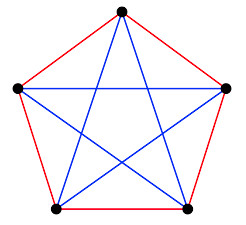
\includegraphics[scale=0.5]{ramsey.jpg}
\end{minipage}

\noindent The Ramsey theory asks a general extremal combinatorics question of this form : For any $s,t \in \mathbb{N}$, what the minimum number $n$ such that there is a guarantee of the form : any $2$-coloring of the edges of the graph $G$ has either a red $K_s$ or a blue $K_t$ in it. This number exists (as proved by Frank Ramsey) and is called the Ramsey Number $R(s,t)$.
In this language, the above argument says $R(3,3) = 6$.
In fact, the existance argument for Ramsey number actually gives the followng upper bound.
\begin{proposition}
$R(s,t) \le R(s,t-1)+R(s-1,t)$.
\end{proposition}

Computing other Ramsey numbers has attracted a lot of attention from combinatorialists. However, we know very little still. $R(s,2)=s$, $43 \le R(5,5) \le 49$ etc. The numbers where $s=t$ are the diagonal entries of the Ramsey matrix (which is natural to imagine given the above). By applyng the above theorem, we have that: $$R(s,s) \le 2^{2s}\sqrt{s}$$

In the rest of this section, we will concetrate on  lower bounds for the diagonal Ramsey numbers. Notice that to show lower bound $R(s,s) \ge n$, we need to show that there is a $2$-coloring of $K_n$ where there is no monochromatic $K_s$. A constructive lower bound of this kind was discovered by Nagy which shows :
$$R(s,s) \ge {s \choose 3}$$

We now apply probabilistic method in order to obtain a stronger lower bound. Erdos, in 1947, introduced
probabilistic methods in his paper {\em Some Remarks on the Theory of Graphs} for proving this lower bound.

\begin{theorem}
The diagonal Ramsey number $R(s,s)$ is at least $\lfloor 2^{\frac{s}{2}}\rfloor$.
Equivalently, when $n=2^{\frac{s}{2}}$, there exists a $2$-coloring of $K_n$ where there is no monochromatic $K_s$.
\end{theorem}
\begin{proof}
As usual, we need to show the existance of a 2-coloring to edges. We set up the following experiment. Color each edge uniformly at random with red or blue. The total number of possible colorings is $2^{n \choose 2}$. The probability of any particular color configuraton is exactly $\frac{1}{2^{n \choose 2}}$.

We need to prove an upper bound of the bad events. Let $S \subseteq n$ of size $s$. Our coloring is bad if $S$ is colored monochromatic under the above coloring.
$$Pr[\textrm{$S$ is monochromatic}] \le \frac{2 \times 2^{{n \choose 2}-{s \choose 2}}}{2^{n \choose 2}} \le 2^{1-{s \choose 2}}$$
$$Pr[\textrm{$\exists S : S$ is monochromatic}] \le
\sum_{S \subseteq [n]:|S|=s} Pr[\textrm{$S$ is monochromatic}] \le {n \choose s}2^{1-{s \choose 2}}$$

If we show that ${n \choose s}2^{1-{s \choose 2}}$ is less than $1$ for $n=2^{s/2}$, then we are done by probablistic argument.

$$
{n \choose s}2^{1-{s \choose 2}} 
\le \frac{n^s}{s!}2^{1-(s/2)+(s^2/s)} 
\le \frac{n^s}{2^{s^2/2}}\frac{2^{1+s/2}}{s!}<1
$$
Hence the proof.
\end{proof}

\begin{exercise-prob}[See Problem Set 2~(Problem~\ref{tournament})]
\begin{show-ps2}{tournament}
A tournament is a directed graph $G(V,E)$ on $n$ vertices where for every pair $(i,j)$, there is either an edge from $i$ to $j$ or from $j$ to $i$, but not both (it represents real tournaments, where we interpret $(i,j)$ directed edge as player $i$ beats player $j$. There is no draw and all pairs of players play a game with each other). 

A tournament T is said to have \textbf{$k$-championship property} if for any set of $k$ vertices in the tournament, there is some vertex in $V$ that has a directed edge to each of those $k$ vertices.

Can $k$-Championship property occur in small tournament graphs? For example, for $k=1$, a tournament will need at least $3$ vertices to have the $k$-Championship property. If $k=2$, a tournament will need at least 5 vertices to have $k$-Championship property.

Show that there are tournments of size $O(k^22^k)$ having $k$-Championship property. [Hint : Consider a random tournament. Fix a set $S$ of $k$ vertices and some vertex $v \notin S$. What is the probability that $v$ is the champion in $S$?]
\end{show-ps2}
\end{exercise-prob}

\begin{exercise-prob}[See Problem Set 2~(Problem~\ref{dominating-set}]
\begin{show-ps2}{dominating-set}
Let $G(V,E)$ be a graph. A set of vertices $D \subseteq V$ is called dominating
with respect to $G$ if every vertex in $V \setminus D$ is adjacent to a vertex in D. $\delta(G)$, the minimum degree amongst $G$’s vertices, is strictly positive. Then $G$ contains a dominating set of size less than or equal to:
$$ \frac{n(1+\log(1+\delta))}{1+\delta} $$
[Hint : Choose a subset $X\subseteq V$ at random (with each vertex in with probability $p$). Let $Y \subseteq V\setminus X$ having no neighbor in $X$. Estimate $X \cup Y$.]
\end{show-ps2}
\end{exercise-prob}
\Week{5}{Pairwise and $t$-wise Independence}

As mentioned in the previous lecture, we do error reduction using limited independence now. We will show that if we use {\em pairwise independent} random variables, then it can still achieve error bounds of the form $\frac{1}{k}$ with only $O(\log n)$ additional random bits.

\section{Pair-wise Independence}
Although not related to expanders, we use this context to introduce one of the basic tools of pseudorandomness - {\em pairwise independent distributions}. We first recall the basic set up about amplification of success probability by repeating the algorithm.\\

\begin{tikzpicture}[shorten >=0.5pt,node distance=0.2cm,on grid,auto]
\node[state,rectangle,minimum width=6cm,minimum height=1.5cm,align=center](q_r)[]{${\cal A}'(x,y_1,y_2, \ldots y_k)$}; 
\node[coordinate](q_0)[right=of q_r,xshift=4cm]{};
\node[coordinate](q_1)[below=of q_r,xshift=0cm,yshift=-1cm]{};
\node[coordinate](q_2)[left=of q_r,xshift=-5cm,yshift=0mm]{};
\path[->](q_r) edge [midway] node {\sc Yes/No} ([xshift=4mm]q_0);   
\draw[->] ([yshift=1mm]q_2) -- ([yshift=1mm]q_r.west)node[midway] {$x \in \{0,1\}^n$};
\draw[->] ([yshift=-2mm,xshift=-25mm]q_1) -- ([yshift=0mm,xshift=-25mm]q_r.south)node[midway,swap] {$y_1$};
\draw[->] ([yshift=-2mm,,xshift=-15mm]q_1) -- ([yshift=0mm,,xshift=-15mm]q_r.south)node[midway,swap] {$y_2$};
\draw[->] ([yshift=-2mm,,xshift=-5mm]q_1) -- ([yshift=0mm,,xshift=-5mm]q_r.south)node[midway,swap] {$y_3$};
\draw[->] ([yshift=-2mm,,xshift=+5mm]q_1) -- ([yshift=0mm,,xshift=+5mm]q_r.south)node[midway,swap] {$\ldots$};
\draw[->] ([yshift=-2mm,,xshift=+15mm]q_1) -- ([yshift=0mm,,xshift=+15mm]q_r.south)node[midway,swap] {$y_k \in \zo^m$};
\end{tikzpicture}

\noindent In the trivial method, we supplied fully independent random strings $y_i \in \zo^m$ for each $i \in [k]$. Now we will allow some dependence among them. A set of random variables $Y_1, Y_2 \ldots Y_m$ is said to be {\em pairwise independent} if for all $i \ne j$, $Y_i$ and $Y_j$ are independent. That is, 
$$\forall a,b : \Pr\left[(Y_i = a) \land (Y_j = b)\right] = \Pr\left[Y_i = a\right] \Pr\left[Y_j = b\right]$$

\paragraph{Constructing Pair-wise Independent Bits:}
We want $k$ ``dependent" random strings produced from fewer number of bits. We first do a simpler setting where instead of strings we ask for bits.

Suppose we want $k$ bits of pairwise independent random bits. How many random bits do we need to spend? And from those pure random bits how do we produce the $k$ bits? These questions are answered by an explicit construction now.

\begin{definition}[\textbf{Construction 1}]
\label{defn:pairwise-indep-bits}
We produce $k = 2^r - 1$ bits from $r$ bits. The $m$ Boolean random variables are indexed by $w \in \{0,1\}^r \setminus \{0^r\}$. The size of the space is $2^r$.
Fix $a \in \{0,1\}^r$, and for any $w \in \{0,1\}^r \setminus \{0^r\}$.
$$Y_w = ( \sum_i a_iw_i )\mod 2$$
\end{definition}
\noindent We need to prove that the set of random variables are pairwise independent.
\begin{claim}
The set of variables $\left\{ Y_w \mid w \in \zo^r \setminus \{0^r\} \right\}$ are pairwise independent.
\end{claim}
\begin{proof}
\noindent We first prove the following two observations about the construction:
\begin{description}
\item{{\sf Subclaim 1 }: For any fixed $w \in \zo^r \setminus \{0^r\}$, the random variable $Y_w$ is uniformly distributed.}
Since $w \ne 0^r$, there must be $i$ such that $w_i = 1$. Consider the non-empty subset of indices: $S = \{ i \mid w_i=1\}$. Hence $Y_w = 0$ if and only if $\card{\{ i \mid a_i = 1 \land i \in S \}}$ is odd. Since the number of sequences $(a_i)_{i \in S}$ with even weight is exactly equal to the number of sequences $(a_i)_{i \in S}$ odd weight ones, the probability is exactly $\half$.
\item{{\sf Subclaim 2 }: For any fixed $w, w
 \in \zo^r \setminus \{0^r\}$, such that $w \ne w'$, the random variable $Y_{w} \oplus Y_{w'}$ is uniformly distributed.}
 This can be argued in a similar way to Subclaim 1. Only thing to note is that 
$$Y_{w} \oplus Y_{w'} = \left( \sum_i a_iw_i \mod 2\right) \oplus \left( \sum_i a_iw_i' \mod 2\right) = \left( \sum_i a_i (w_i \oplus w_i') \right)\mod 2 = Y_{w \oplus w'}$$
where $w \oplus w'$ is the bit-wise $\oplus$ of the bits in $w$ and $w'$.
Since $w \ne w'$, $w \oplus w' \in \zo^r$ and $w \oplus w' \ne 0$, and hence the same argument as in claim 1 applies.
\end{description}
Now we are ready to argue pairwise independence of $Y_w$ and $Y_{w'}$. Let $w \ne w' \in \zo^r$. We need to show that for $\Pr\left[(Y_w = a) \land (Y_{w'} = b)\right] = \frac{1}{4}$. Let $\Pr\left[(Y_w = 0) \land (Y_{w'} = 1)\right] = p$. Since $w \ne w'$, there is an $i \in[r]$ such that $w_i \ne w_i'$. Hence, 
\begin{eqnarray*}
\text{ Note that, } \half = \Pr\left[(Y_w = 0)\right] & = & \Pr\left[(Y_w = 0) \land (Y_{w'}=0)\right]+\underbrace{\Pr\left[(Y_w = 0) \land (Y_{w'}=1)\right]}_\text{$p$} \\
\implies \Pr\left[(Y_w = 0) \land (Y_{w'}=0)\right] & = & \half-p  \\
\text{ Using this, }\half = \Pr\left[(Y_{w'} = 0)\right] & = & \underbrace{\Pr\left[(Y_{w'} = 0) \land (Y_{w}=0)\right]}_{\half-p}+\Pr\left[(Y_{w'} = 1) \land (Y_w=1)\right] \\
\implies \Pr\left[(Y_w = 1) \land (Y_{w'}=0)\right] & = & p 
\end{eqnarray*}
Hence, $\Pr\left[ Y_{w} \oplus Y_{w'} = 1\right] = 2p$. Because of subclaim 2, this gives $p = \frac{1}{4}$ and hence shows: 
$$\Pr\left[(Y_w = a) \land (Y_{w'} = b)\right] = \frac{1}{4} = \Pr\left[(Y_w = a)\right] \Pr \left[(Y_{w'} = b)\right]$$
\end{proof}

\paragraph{Constructing Pair-wise Independent Strings:}
While easy to analyze, the disadvantage of the inner product construction in the previous construction is that it outputs bits. However, for our purposes of amplification, we require pairwise independent strings $y_1, y_2, \ldots y_k \in \{0,1\}^m$. We now show a second construction which yields strings instead.

\begin{definition}[\textbf{Construction 2}]
Fix $q \ge k$. Choose $\alpha, \beta \in \F_q$ uniformly at random. Output $Y_w = \alpha w+\beta$ where $w \in \F_q$. This produces $q$ bits from $2\log q$ bits as seed. The size of the space is $q^2$.
\end{definition}

\begin{claim}
The random variables $\{ Y_w \mid w \in \F_q\}$ are pairwise independent.
\end{claim}
\begin{proof}
Let $w \ne w' \in \F_q$. Consider $a,b \in \F_q$. We need to show 
\begin{equation}
\Pr\left[(Y_w = a) \land (Y_{w'} = b)\right] = \Pr\left[(Y_w = a)\right] \Pr \left[(Y_{w'} = b)\right]
\label{eqn:pairwiseindep}
\end{equation}

\begin{description}
\item{\sf Estimating RHS:}
We first observe that, for a fixed $w \in \F_q$, $\Pr\left[(Y_w = a)\right] = \frac{1}{q}$. To see this, note that for any $\alpha \in \F_q$, there is exactly one $\beta \in \F_q$ which satisfies $\alpha w + \beta = a$. Hence, there are $q$ pairs $(\alpha,\beta)$ (among the $q^2$ possible pairs) which satisfies $\alpha w+\beta = a$. Hence RHS of Equation~\ref{eqn:pairwiseindep} is $\frac{1}{q^2}$.
\item{\sf Estimating LHS:}
The event $(Y_w = a) \land (Y_{w'} = b)]$ translates to the pair of equations: $\alpha w + \beta = a \textrm{ and } \alpha w' + \beta = a$.
Since $w, w'$ (and $w \ne w'$) and $a,b$ are fixed, this is possible only for a unique pair of values $(\alpha, \beta) \in \F_q \times \F_q$. In other words the matrix equation:
\[
\begin{pmatrix}
w & 1 \\
w' & 1
\end{pmatrix}
\begin{pmatrix}
\alpha \\
\beta
\end{pmatrix}
=
\begin{pmatrix}
a \\
b
\end{pmatrix}
\textrm{ and hence, }
\begin{pmatrix}
\alpha \\
\beta
\end{pmatrix}
=
\begin{pmatrix}
w & 1 \\
w' & 1
\end{pmatrix}^{-1}
\begin{pmatrix}
a \\
b
\end{pmatrix}
\]

defines a bijection between the set of $(\alpha,\beta)$ pairs and $(a,b)$ pairs. Hence, for every $(a,b) \in \F_q \times \F_q$, there is only one $(\alpha,\beta)$ (out of the $q^2$ choices) which will make $(Y_w = a) \land (Y_{w'} = b)$. Hence LHS of the Equation~\ref{eqn:pairwiseindep} is $\frac{1}{q^2}$.
\end{description}
\end{proof}

\begin{exercise-prob}[See Problem Set 2~(Problem \ref{matrix-family})]
\begin{show-ps2}{matrix-family}
\begin{enumerate}[(a)]
\item For an $n \times m$ matrix $A$ with Boolean entries and
$b \in \zo^n$, define a function $h_{A,b} : \zo^m \to \zon$ by
$h_{A,b}(x)= (Ax + b) \mod 2$ where the modulo 2 is applied component-wise. Show that 
$$H_{m,n} = \{h_{A,b} \mid A \in \zo^{n \times m} \textrm{ and } b \in \zo^n\}$$
is a pairwise independent family of functions. Compare the number of random bits needed to generate a random function in $H_{m,n}$ to the construction that we did in class.
\item A matrix $A$ is a {\em Toeplitz matrix} if it is constant on
diagonals, i.e., $A_{i+1,j+1} = A_{i,j}$ for all $i$, $j$. Show that even if we restrict the family $H_{m,n}$ in Part 1 to only include $h_{A,b}$ for Toeplitz matrices $A$, we still get a pairwise independent family. How many random bits are needed now?
\end{enumerate}
\end{show-ps2}
\end{exercise-prob}

\section{Error Reduction using Pairwise Independence}
We first describe the algorithm for amplification first. We choose $q = 2^m$ : elements in $\F_q$ can be interpreted as strings of length $m$.

\begin{algorithm}
\label{alg:pairwise-indep-amplification}
\caption{(${\cal{A}'}$) : input $x \in \{0,1\}^n$} 
\begin{algorithmic}[1]
\State {\em count} $\gets 0$. 
\State Choose a pair $(\alpha,\beta) \in \F_q \times \F_q$ uniformly at random. \Comment{(Uses $2m$ random bits)}. 
\State Let $y_1, y_2, \ldots y_k$ be the first $k$ elements of the pairwise independent space 
\vspace{-3mm}
$$\{ \alpha w + \beta \mid w \in \F_q \}$$
\vspace{-10mm}
\For{\texttt{each $i \in [k]$}}
	\State If ${\cal{A}}(x,y_i)$ accepts, if so increment {\em count}
\EndFor
\State If ~[{\em count} $> \frac{k}{2}$]~ then output {\sc Yes} else output {\sc No}.
\end{algorithmic}
\end{algorithm}
One immediate remark is that although it may look like we are wasting bits by generating more pairwise independent random bits than required, we cannot make use of them efficiently anyway since there are $2^m$ many of them.

We now prove the correctness lemma which indicates that if we need to reduce the error probability to $1/t$, then we need to repeat the algorithm for $k=O(t)$ times.
\begin{lemma}
\label{lem:paiewise-amplification}
The probability of error for $\calA'$ is bounded by:
$$\Pr\left[\calA' \textrm{ errs }\right] \le \left(\frac{1}{\delta^2}\right)\frac{1}{k} \textrm{~~~~where $\delta = \frac{1}{2}-\epsilon$}$$
\end{lemma}
\begin{proof}
As in the previous cases, for a given input $x \in \zon$, we define $B$ to be the set of bad random strings - which makes the algorithm err on input $x$. We need to understand the probability that majority of $y_i \in B$. For this, let us define the indicator random variable.
\[
    Y_i = 
\begin{cases}
    1 & \text{if $y_i \in B$} \\
    0 & \text{otherwise}
\end{cases}
\]
$\E[Y_i] = Pr[y_i \in B] = \epsilon$. We will define a translation of $Y_i$ to make the expectation $0$. Define $Z_i = Y_i - \epsilon$. Notice that $\E[Z_i]=0$. In terms of these random variables, to bound the error for $\calA'$, we want to analyze the probability that:
$$\Pr \left[ \sum_{i=1}^k Y_i > \frac{k}{2}\right] = \Pr \left[ \sum_{i=1}^k Z_i > k\left(\frac{1}{2}-\epsilon\right) \right] = \Pr \left[ \sum_{i=1}^k Z_i > \delta k \right] =\Pr \left[ Z > \delta k \right] $$
where $Z = \sum_{i=1}^k Z_i$.
The random variable $Z$ has expectation $0$ and we want to estimate the probability that it is greater than $\delta k$. A natural situation is to apply Markov's inequality\footnote{For a random variable $X$ which takes only positive values in $\mathbb{R}$, $\Pr[X > a] \le \frac{\E[X]}{a}$} which helps us estimate such a tail bound for positive random variables.
Hence we plan to upper bound:
\begin{eqnarray*}
\Pr \left[ Z > \delta k \right] \le \Pr[Z^2 > \delta^2 k^2] \le \frac{\E[Z^2]}{\delta^2k^2}
\end{eqnarray*}
Hence we need to estimate $\E[Z^2]$:
\begin{eqnarray*}
\E[Z^2] = \E\left[ \left(\sum_{i=1}^k Z_i\right)^2 \right] = \sum_{i=1}^k \E\left[Z_i^2\right] + 2\sum_{i<j} \E[Z_iZ_j] & \le & \sum_{i=1}^k \E\left[Z_i^2\right] + 2\sum_{i<j} \E[Z_i]\E[Z_j] \\
& \le & k \textrm{~~~~~~~~$\because \E[Z_i] = 0$ and $\E[Z_i^2] \le 1$}
\end{eqnarray*}
Hence we have :
$$\Pr \left[ Z > \delta k \right] \le \frac{1}{\delta^2 k}$$
thus completing the proof.
\end{proof}
\begin{remark}
As mentioned earlier, if we need $\frac{1}{t}$ as an upper bound on the error probability, we need to run the algorithm for $k=O(t)$ times.
\end{remark}


\begin{exercise}
Let $X$ be a random variable and $\E[X] = \mu$ be the expectation. Variance captures the expected square deviation from the mean $\mu$. That is $\V{X}$ is defined as $\E[(X-\mu)^2]$. It can be shown to be equal to $\E[X^2]-(\E[X])^2$ and that $\V{aX} = a^2\V{X}$. And more importantly, when the random variables $X_1, X_2, \ldots X_n$ are pairwise independent, then show that:
$$\V{X_1+X_2+\ldots+X_n} = \V{X_1}+\V{X_2}+\ldots+\V{X_n}$$
(Hint: Use the technique used in the proof of Lemma~\ref{lem:paiewise-amplification})

Provide an example that shows that the variance of the sum of two random variables is not necessarily equal to the sum of their variances, when the random variables are not independent. Indeed, one dramatic example when $n=2$ is to take $X_2 = -X_1$. Find less dramatic ones !.
\end{exercise}


\section{Derandomization using Pairwise Independent Bits}

We now show an application of pairwise independent bits that we generated (instead of strings) in earlier section. This also will demonstrte algorithmic specific derandomization that we can do, at times, for certain problems. 

Recall the {\sc MaxCut} problem. A cut in a graph is a partition of vertex set $V$ into two $(S,\bar{S})$ and the size of a cut is the number of edges that go across the cut $|E(S,\overline{S})|$. The {\sc MaxCut} problem is as follows : \textit{Given a graph $G(V,E)$ output the maximum cut in the graph.}

We will first give a simple randomized algorithm for the problem. Note that this is not a decision problem and hence the measure of how good the algorithm is based on the expected size of the cut that the algorithm outputs.

\begin{algorithm}
\label{alg:maxcut-randomized}
\caption{(${\sc MaxCutAlgo}$) : input $G(V,E)$, $|V|=n$} 
\begin{algorithmic}[1]
\State $S \gets \phi$. 
\For{each $w \in [V]$}
	\State Choose $b_w \in \zo$ uniformly at random.
	\State If ($b_w = 1$) then add $w$ to $S$.
\EndFor
\State Output the cut $(S,\bar{S})$.
\end{algorithmic}
\end{algorithm}

We quickly analyse the algorithm. For each edge $e=(u,v) \in E$ define the random variable $X_e$ which will be $1$ if the above algorithm makes the edge contribute to the cut and $0$ otherwise.
For a given edge the expected value of this random variable is :
\begin{equation}
\label{eqn:maxcut-exp}
\E[X_e] = \Pr[X_e = 1] = \Pr[(u \in S) \land (v \in \bar{S})] + \Pr[(u \in \bar{S}) \land (v \in S)] = \frac{1}{4}+\frac{1}{4} = \half
\end{equation}

\noindent The expected size of the cut then is obtained by estimating the expectation of $X = \sum_{e \in E} X_e$:
$$\E[X] = \E\left[\sum_{e \in E} X_e\right] = \sum_{e \in E} \E[X_e] = \half |E| \ge \half |OPT|$$
where $OPT$ is the size of the maximum cut in the graph and it can be at most $|E|$. Thus the above algorithm gives a $\half$ approximation for the {\sc MaxCut} problem on expectation.

The algorithm uses $O(n)$ random bits where $n=|V|$. We claim that the analysis of the algorithm still guarantees the expected size of the cut to be $\half|OPT|$ even if we do not use pure randombits, but instead supply the pairwise indepednent randbom bits we generate (from definition~\ref{defn:pairwise-indep-bits}). We choose $n = 2^r - 1$ which uses $r = O(\log n)$ seed in order to choose from the pairwise independent space that we constructed.
Let the bits that we provided by $b_1, b_2, \ldots b_n$ produced from construction ~\ref{defn:pairwise-indep-bits}.

\noindent Equation~\ref{eqn:maxcut-exp} can be rederived as:
\begin{eqnarray*}
\E[X_e] = \Pr[X_e = 1] & = & \Pr[(b_u=1) \land (b_v=0)] + \Pr[(b_u=0) \land (b_v=1)] \\
& = & \Pr[b_u=1]\Pr[b_v=0] + \Pr[b_u=0]\Pr[b_v=1] = \frac{1}{2}.\frac{1}{2}+\frac{1}{2}.\frac{1}{2} = \half
\end{eqnarray*}
were we use the pairwise independence in the third equality (which we wrote earlier because of full independence.

Hence, we have an algorithm which uses $O(\log n)$ random bits (call the string $y'$) and provides a $\half$-approximation for the maximum cut on expectation. Hence there must be a random string setting for $y'$ which produces the $\half$-approximation such that $\card{E(S,\bar{S})} \ge \half|OPT|$. Hence, this leads to a polynomial time deterministic algorithm, which runs over all the possible assignments for the string $y'$ (only $\poly(n)$ in number) and runs the algorithm using each setting of $y'$ as random string, and outputs the maximum sized cut produced. By the above argument, this algorithm is guranteed to produce a $\half$-approximation for the maximum cut in the graph.

\begin{exercise}
%-prob}[See Problem Set 3~(Problem \ref{ramsey-graph})]
%\begin{show-ps3}{ramsey-graph}
Recall the discussion on Ramsey graph's where we applied probablistic method to show bounds on Ramsey number $R(k,k)$. Let us define a graph to be a \textit{$k$-Ramsey graph} if it has no clique or independent set of size at least $k$. We had shown by the probabilistic method that there exists a graph on $n$ vertices that $O(\log n)$-Ramsey. An interesting open problem is to give an \textit{explicit} construction of a $O(\log n)$-Ramsey graph. The best known construction runs in time $O(2^{2^{\log^\epsilon n}})$ for some small $\epsilon=0.99$. In this problem you are asked give a construction for $O(\log n)$ Ramsey graph that runs in time $O(n^{\log^2 n})$. [Hint : Check if full independence of random choices is necessary in our proof by probabilistic method. Show that the proof actually gives a set of $O(n^{\log^2 n})$ graphs, one of which is guaranteed to be $O(\log n)$-Ramsey]
%\end{show-ps3}
%\end{exercise-prob}
\end{exercise}

\begin{curiousity}
The best approximation ration for maximum cut problem is not $\half$. It is $0.878$, and it comes from the semidefinite programming (SDP) relaxation for maxcut problem LP. Define $n+m$ variables $x_u$ for each $u \in V$ and $e_{uv} \in E$. These variables are supposed to represent the information $e_{uv} = 1$ if and only if $(u,v)$ is in the cut, and $x_u = 1$ if and only if $u \in S$. The LP objective function is to maximise $\sum_{(u,v) \in E} e_{uv}$ subject to the constraints (1) $\forall u,v \in E$, $e_{uv} \le x_u+x_v$ and $e_{uv} \le 2-(x_u+x_v)$, (2) all of them are Boolean variables. The idea due to \cite{GW95} is to relax this condition (2) by using vector valued variables (rather than Boolean). Not only that this relaxation can be solved efficiently, but \cite{GW95} gave a method of rounding the variables to Boolean values and proving that the approximation ratio is atleast $0.878 \ldots$.

Complementing this, an optimal inapproximability result was proven for {\sc MaxCut} by \cite{Kho07}, based on a conjectured hardness for the approximation problem known as the label cover problem (this is also called the {\em unique games conjecture}~(UGC) - see ~\cite{Kho10}).
\end{curiousity}

\Week{6}{Expander Graphs : Existence and Algebraic Constructions}

We now use the tools that we have developed in order to construct show existance and then explict constructions of expanders. We recall the definition of expanders from Section~\ref{sec:intro-expanders} but now we make the paramters more precise.

\begin{definition}{(\bf Expander Graphs)}
A graph $G(V,E)$ is said to be a $(n,d,\alpha,\beta)$-expander if, $|V|=n$, it is $d$-regular, and every $S \subseteq V$ such that $|S| \le \alpha|V|$, the number of new neighbors $|N(S)\setminus S| \ge \beta d|S|$.
\end{definition}

\noindent {\bf Note :} We are changing the notation slightly from what we followed in the lecture to ensure that both $\alpha$ and $\beta$ are in $(0,1)$.

\noindent A weaker setting is to consider bipartite graphs where we insist the above only for subset of vertices from one side of the bipartite graph, so that $|N(S)\setminus S| = |N(S)|$ since there is no edge from a set to itself in this case.

\begin{definition}{(\bf Bipartite Expander Graphs)}
A graph $G(U \cup V,E)$ is said to be a $(n,d,\alpha,\beta)$-expander if, $|U|=n$, it is $d$-regular and every $S \subseteq U$ such that $|S| \le \alpha|U|$, the number of new neighbors $|N(S)| \ge \beta d|S|$.
\end{definition}
\section{Existence of Left regular Bipartite expanders}

What kind of parameters should we expect for expanders and what do we need. Looking at the possible application in the case of randomness efficient amplification, we would like the degree of the graph to be much much smaller than the number of vertices (ideally a constant). It is natural to keep the graph regular because then the mathematical constraints are easier to handle (as we will see). We can also allow the graph to have multiple edges between two vertices since we do not require the neighbors to be distinct.

Ideally, we would want $\beta$ to be as close to $1$ as possible. In fact, for many of the applications, it is enough to have $\beta > \half$. We will show the existance of a $(n,d,\alpha,\frac{d-2}{d})$ expander which will be good as long as $d \ge 5$. We show the following theorem (which not only shows existence but also implies abundance).

\begin{theorem}
For every constant $d$, there is an $\alpha > 0$ such that for all large enough $n$: a uniformly chosen random bipartite graph $G(U \cup V, E)$ which is left $d$-regular and $|U|=|V|=n$, is an $(n,d,\alpha,\frac{d-2}{d})$ with probability at least $\half$.
\end{theorem}
\begin{proof}
We spell out the details of the experiment first. Each vertex $u \in U$ is assigned $d$ neighbors from the right side (with replacement) chosen uniformly at random, each indepedently. 

We will compute probability that the outcome of the experiment is not an expander and show that this probability is less than $\half$.

\noindent The graph is not an expander with the required parameters if there exists a set $S \subseteq U$, $|S|\le \alpha n$ such that $|N(S)| < (d-2)|S|$. We will use union bound over all such $S$.
$$
\Pr\left[\begin{array}{l}
\exists S \subseteq U, \textrm{ with } |S|\le \alpha n \\
\textrm{ s.t. } |N(S)| < (d-2)|S|
\end{array}
\right] 
\le \bigsum_{\substack{S \subseteq U\\
|S|\le \alpha n}} Pr[|N(S)| < (d-2)|S|] 
\le \bigsum_{k=1}^{\alpha n} {n \choose k} p_k
$$
where $p_k$ is the upper bound we hope to derive for $Pr[|N(S)| < (d-2)|S|]$ for any $S \subseteq U$ with $|S|=k$.

Now, we just need to estimate $p_k$. First, we observe that the only way the number of neighbors of a vertex $u \in U$ can go below $d$ is when the random choice ends up choosing the same vertex $v \in V$ more than once in the experiment for $u$. To use this, let $M=\{\{v_1, v_2, \ldots v_{kd}\}\}$ be the multiset of $kd$ outcomes when $d$ neighbors are chosen uniformly at random for each of the vertices in $S$. If $|N(S)| < (d-2)k$, then it must be because there exists $2k$ repetitions in this sequence. The repetitions can be any of the $2k$ sub-multi-subsets out of these $kd$ neighbors. We apply union bound over all the subsets. Thus,
\begin{eqnarray*}
p_k = \Pr\left[\begin{array}{l}
\exists T \subseteq M, \textrm{ with } |T|=2k \\
\textrm{ s.t. all elements in $T$ are repeats}
\end{array}
\right] 
& = & \bigsum_{\substack{{T \subseteq M}\\|T|=2k}}
\Pr\left[\begin{array}{l}
\textrm{all elements in $T$}\\
\textrm{are repeats}
\end{array}
\right] \\
& \le & \bigsum_{\substack{{T \subseteq M}\\|T|=2k}} \left(\frac{kd}{k}\right)^{2k}
\le {kd \choose 2k}\left(\frac{kd}{n}\right)^{2k}
\end{eqnarray*}
The last inequality is by noting that the probability of any particular element repeating is at most $\frac{kd}{n}$ (the worst case is for the last element in $T$ chosen). Hence,
\begin{eqnarray*}
\Pr\left[\begin{array}{l}
\exists S \subseteq U, \textrm{ with } |S|\le \alpha n \\
\textrm{ s.t. } |N(S)| < (d-2)|S|
\end{array}
\right] 
&\le &\bigsum_{k=1}^{\alpha n} {n \choose k}  {kd \choose 2k}\left(\frac{kd}{n}\right)^{2k} \\
& \le & \bigsum_{k=1}^{\alpha n} \left(\frac{ne}{k}\right)^k \left(\frac{kde}{2k}\right)^{2k} \left(\frac{kd}{n}\right)^{2k}
\textrm{~~~~~~~~using ${n \choose k} \le \left(\frac{ne}{k}\right)^k$} \\
& \le & \bigsum_{k=1}^{\alpha n} \left(\frac{e^3d^4k}{4n}\right)^k \le \bigsum_{k=1}^{\alpha n} 4^{-k} \textrm{~~~~~~~~~~~choose $\alpha = \frac{1}{e^3d^4}$} \\
& < & \half
\end{eqnarray*}
Hence the proof.
\end{proof}

\section{Variants of Expanders}
The discussion in the beginning of the previous section motivates the definition of variants of expander definition. What we defined in the previous section is called the boundary expansion where we insisted that $|N(S)\setminus S|$ must be large. We define two variants of the same.
\begin{definition}[{\bf Vertex Exapansion}]
A graph $G(V,E)$ is said to be a $(n,d,\alpha,\beta)$-expander if, $|V|=n$, it is $d$-regular, and every $S \subseteq V$ such that $|S| \le \alpha|V|$, the number of new neighbors $$|N(S)| \ge \beta d|S|$$
\end{definition}
Notice that when we consider bipartite graphs $N(S) \cap S \ne \phi$, but still the above definition is stronger since it asks for all $S \subseteq V$ and not the subsets only in one side.
\begin{definition}[{\bf Edge Exapansion}]
A graph $G(V,E)$ is said to be a $(n,d,\alpha,\beta)$-expander if, $|V|=n$, it is $d$-regular, and every $S \subseteq V$ such that $|S| \le \alpha|V|$, the number of new neighbors
\begin{equation}
|E(S,\overline{S})| \ge \beta d|S|
\label{eqn:edge-expansion}
\end{equation}
\end{definition}

Viewing it from the graphs side, we can define the edge expansion ratio of a $d$-regular graph $G$ as,

$$h(G) = \min_{\{S \subseteq [n] :  
|S| \le \frac{n}{2}\}}\frac{|E(S,\overline{S})|}{d|S|}$$

In other words, for a given graph $G$, what is the smallest $\beta$ for which it satisfies Equation~\ref{eqn:edge-expansion}. The answer is the edge expansion ratio $h(G)$.

\begin{exercise}
Let $n,d \in \mathbb{N}$, $\alpha, \beta > 0$.
Every $(n,d,\alpha,\beta)$-boundary-expander is also a $(n,d,\alpha,\frac{\beta}{d})$-edge-expander. Conversely, every $(n,d,\alpha,\beta)$-edge-expander is also a $(n,d,\alpha,\beta)$-boundary-expander.
\end{exercise}
\begin{exercise-prob}[See Problem Set 3~(Problem~\ref{expander-defn})]
\begin{show-ps3}{expander-defn}
Let $G=(V,E)$ be a graph. For every subset $S$ of its vertices $V$ we say, that vertex $v \in V\setminus S$ is a neighbor of $S$ if $E(S,{v}) \ge 1$, an odd neighbor of $S$ if $E(S,{v})$ is odd, a unique neighbor of $S$ if $E(S,{v})=1$. Further, we denote:
\begin{eqnarray*}
B(S) & = & \{v \in V \setminus S \mid v \textrm{ is a neighbor of } S\}\\
B_{odd}(S) & = & \{v \in V \setminus S  \mid v \textrm{ is an odd neighbor of } S\}\\
B_{unique}(S) & = & \{v \in V \setminus S \mid v \textrm{ is a unique neighbor of } S\}
\end{eqnarray*}
A graph $G$ is said to be an $(n,d,\alpha,\beta)$-odd-neibhor (resp. unique-neighbor) expandor if for every $S \subseteq V$, where $|S| \le \alpha n$, the set $B_{odd}$ (resp. $B_{unique}$)  is of size at least $\beta d |S|$.
\begin{enumerate}[(a)]
\item Show that every $(n,d,\alpha,\beta)$ unique-neighbor expander is an $(n,d,\alpha,\beta)$ odd-neighbor expander.
\item Show that every $(n,d,\alpha,\beta)$ odd-neighbor expander is also an $(n,d,\alpha,\beta)$ boundary expander.
\item Show that every $(n,d,\alpha,\frac{1}{2}+\frac{\epsilon}{d})$-boundary expander is also a $(n,d,\alpha,\frac{2\epsilon}{d})$-unique-neighbor expander.
\end{enumerate}
\end{show-ps3}
\end{exercise-prob}

It is usually assumed that $\alpha = \half$. In fact, if we have an edge expander with $\alpha = \half$, then we have one for larger $\alpha$ as well. The following exercise will ascertain that.

\begin{exercise-prob}[See Problem Set 3~(Problem~\ref{expander-alpha})]
\begin{show-ps3}{expander-alpha}
Let $n \in \mathbb{N}$ and $\half < \alpha < \frac{n-1}{n}$, and $G(V,E)$ by an $(n,d,\half,\beta)$ edge-expander, then $G$ is also an $(n,d,\alpha,(1-\alpha)\beta)$ edge expander.
\end{show-ps3}
\end{exercise-prob}

We showed in the last section that, bipartite expanders exist with good parameters. Now we will show edge-expanders exists using the expectation method. The following problem is designed for that.

\begin{exercise-prob}[See Problem Set 3~(Problem~\ref{expander-exists})]
\begin{show-ps3}{expander-exists}
Through the following steps, show that there exists a family of $(n,d,\half,\beta)$ edge-expander.
\begin{enumerate}[(a)]
\item Choose $\beta$ later. Choose a random $d$-regular graph on $n$ vertices. Let $S \subseteq V$, with $s=|S| \le \frac{n}{2}$. Define the random variable $E_S = |E(S,V\setminus S)|$. Let $0 \le k \le \beta d |S|$. Prove that if $sd-k$ is an odd number, then, $\Pr[E_S = k] = 0$.
\item If $sd-k$ is even, then show that 
$$\Pr[E_S=k] \le \left(\frac{3s}{2n}\right)^{ds/4}
\textrm{ \hspace{1cm} Use ${a \choose b} \left( \frac{ae}{b}\right)^b$ and choose $\beta$ such that $\left(\frac{e}{\beta}\right)^{4\beta} \le \frac{9}{8}$} 
$$
The intuition behind this part is that every edge with one endpoint in the subset $S$ has probability roughly $s/n$ that the other endpoint is contained in $S$
as well.
\item Use the previous part to show that :
$$ \Pr\left[E_S < \beta ds\right] \le \left(\frac{5s}{3n}\right)^{ds/4} \textrm{ \hspace{1cm} Assume $d \ge 140$ and do approximations.}$$
\item Prove that the probability that there exists a set of size at most $\frac{n}{2}$, is $<1$. Hence conclude the theorem.
\end{enumerate}
\end{show-ps3}
\end{exercise-prob}

\section{Marguilis-Gabber-Galil Expander}

Although we showed the existence arguments only for left-regular bipartite expanders, similar arguments exists for other kinds of objects in the above lists too. Now we turn into explicit constructions of families of expander graphs.

There are two major approaches to constructing expander graphs. One regime is purely algebraic, in which the expander graphs are defined over algebraic structures and connectivity is determined by algebraic properties. They are very easy to describe (more formally, they are very explicit). However, the arguments that they are indeed expanders is more complicated (in fact, even beyond the scope of this course, in terms of background required). Hence we will not be proving that they are expanders, but we will describe them. 

The other regime of constructions is more combinatorial and are based on graph operations. It takes care to make them explicit, but the proof of expansion is somewhat more amenable for the background of this course.

\begin{description}
\item{\bf Marguilis-Gabber-Galil Expander:}
First family was studied by \cite{Mar73} where the proof of expansion was based on representation theory and did not provide any specific bound on the expansion ratio $h$. Later \cite{GG81} derived such a bound
using harmonic analysis.

We now describe the family which is on $n^2$ vertices 
is $V = \Z_n \times \Z_n$. The neighbors of the vertex $(a,b) \in V$ are :
$$N(a,b) = \left\{\begin{array}{l}
(a+b,b)\\
(a-b,b)\\
(a,b+a)\\
(a,b-a)\\
(a,b+a+1)\\
(a,b-a+1)\\
(a+b+1,b)\\
(a-b+1,b)
\end{array}
\right\}
$$
\item{\bf Expanders from Number Theory:}
These graphs can be constructed when the number of vertices expected is a prime. The family of $3$-regular contains $p$-vertex graphs for every prime $p$. Here $V = \Z_p$, and for a vertex $a \in V$: 
$$N(a) = \{a+1,a-1,a^{-1}\}$$
where all operations are in $\Z_p$.
\end{description}

Although we will not describe the proof of expansion of the above graphs, they all go through a special connection between edge expansion and the spectrum of a graph. We quickly introduce this in the next section.

\section{Spectral Expansion}
\label{sec:spectral-expansion}

We consider simple graphs for simplicity. For a $d$-regular undirected graph, define the normalized adjacency matrix as follows:
$$
A_{uv} = \left\{ \begin{array}{ll}
\frac{1}{d} & (u,v) \in E \\
0 & \textrm{ otherwise }
\end{array}
\right.
$$
Since $G$ is undrected, the matrix is symmetric and hence the eigen values of the matrix are all real numbers\footnote{We reviewed the basic related definitions about eigen values in the lecture, but we are not writing them here to avoid digression.}. Since the graph is $d$-regular, the matrix is also doubly stochastic. Hence the all $1$ vector (and any scalar multiple of it) is an eigen vector and $1$ is the eigen value corresponding to it. The largest eigen value of a doubly stochastic matrix is $1$ (Prove this as an exercise !). Notice that there are at most $n$ eigen values and some of them could be with higher multiplicity.

All eigen values of the matrix are in the interval $[-1,1]$. Folding this range, by taking absolute values, 
let the absolute values of the eigen values of the normalized adjacency matrix\footnote{We denote them as $\lambda_i(G)$.} $1=\lambda_1 \ge \lambda_2 \ge \lambda_3 \ldots \lambda_k \ge 0$ where $k \le n$. This sequence is called the {\em spectrum of the graph}. Spectrum of a graph contains surprising information about the combinatorial structure of the graph. Spectral graph theory studies the relationship between spectrum and combinatorial properties of the graph (for example, connectedness, bipartiteness, number of connected components).

The gap between the first two eigen values is called the \textbf{spectral gap} of a graph. And a $d$-regular graph is called a spectral expander if the second largest eigen value $\lambda_2(G)$ is below $1$ by a constant gap. More formally:

\begin{definition}[\textbf{Spectral Expanders}]
A $d$-regular graph is said to be $(n,d,\lambda)$ spectral expander if $\lambda_2(G) \le \lambda$. Equivalently, the spectral gap of the graph is at least $1-\lambda$.
\end{definition}

There are two questions that we will address now. First of all, why study spectral expansion? We show that spectral expanders in fact have edge expansion too. Thus to show that a graph is an edge expander, it suffices to show that it is an spectral expander. This is the approach taken for proving that the algebraic constructions the we described in the previous section are expanders. However, the way to achieve that is still through harmonic anlaysis and number theory etc.

The second question is to do the curious statement that spectral expanders are in fact edge expanders too. We try to make this precise through the following statement.

\begin{theorem}[\textbf{Spectral Expansion Implies Edge Expansion}]
If $G$ is an $(n,d,\lambda)$ spectral expander, then it is also a $(n,d,\half,\frac{1-\lambda}{2})$ edge expander.
\end{theorem}

In fact, the converse of the above theorem is also true. We show the formal proof of the above statement in the next lecture (in fact, a much stronger form too) with the converse.

In the rest of this lecture, we make an informal handwavy attempt to justify why one should expect such a connection between spectral expansion and edge expansion. The argument is through the idea of random walks on graphs. A random walk on a graph $G$ is a random experiment performed on the $G$ as follows. Starting from a vertex $v$ and choosing the next neighbor among the neighbors of the current vertex. The walk produces a sequence of vertices. The relevant question is - fix an integer $\ell \in \N$ - {\em what does the distribution of the $\ell^{th}$ vertex in the walk look like?} Of course, the answer depends on the graph. Then the question is what parameter of the graph governs the distribution of the vertex after $\ell$ steps of the walk? Are there graphs for which it will be the uniform distribution or even close to uniform distribution.

If the distribution gets closer and closer to uniform - then it is termed as {rapid mixing of the random walk}. The rate at which it gets closer is a paramter. If there was no edge expansion, then we would have had random walks initiating from the set $S$ (which did not have edge expansion) to not get distributed uniform easily. Hence we would expect random walks to not mix fast. In the contrapositive, this says that, intuitively, \textit{if random walks in a graph mixes well, then there must be edge expansion in the graph}.

Now we need to address the question, why does spectral gap imply that random walks in the graph mix well? This has a very cute linear algebraic reason. To answer this at least informally, we take an example graph. To keep track of the distribution that evolves with the length of the walk, we denote by $p_i \in \mathbb{R}^n$ the probability distribution vector after the $i$th step in the random walk.

Suppose we are starting from the topmost vertex. Let $X_i$ be the random variable denoting the vertex after the $i^{th}$ step. Define the vector $p_i$, with entries as $p_i[j] = \Pr[X_{i} = j]$.
\hspace{-6mm}\begin{minipage}{0.75\linewidth}
\begin{center}
\begin{tabular}{c|cccccccc}
& 1 & 2 & 3 & 4 & 5 & 6 & 7 & 8 \\
\hline
$p_0$ & 1   & 0    & 0    & 0   & 0 & 0 & 0 & 0 \\
$p_1$ & 0   & 0.5  & 0.5  & 0   & 0 & 0 & 0 & 0 \\
$p_2$ & 0.5 & 0    & 0    & 0.5 & 0 & 0 & 0 & 0 \\
$p_3$ & 0   & 0.42 & 0.42 & 0   & 0.17 & 0 & 0 & 0 \\
$\vdots$ &   &  & $\vdots$ &    & & $\vdots$ & & \\
\end{tabular}
\end{center}
$$p_{i+1}[j] = \Pr[X_{i+1} = j] = \bigsum_k \Pr[X_{i} = k]\Pr[\textrm{ $(k,j)$ edge is chosen }] $$
This implies that $p_{i+1} = Ap_i$. 
\end{minipage}
\begin{minipage}{0.05\linewidth}
~
\end{minipage}
\begin{minipage}{0.15\linewidth}

\SetGraphUnit{1}
\GraphInit[vstyle=Classic]
\SetUpVertex[FillColor=blue!60]  
\tikzset{VertexStyle/.append style={minimum size=2pt,inner sep=1pt}}
\begin{tikzpicture}
  \Vertex[x=4,y=1,L=1]{A}
  \Vertex[x=4,y=-1,L=4]{B}
  \Vertex[x=5,y=0,L=3]{C}
  \Vertex[x=3,y=0,L=2]{D}      
  \Vertex[x=4,y=-2,L=5]{E}
  \Vertex[x=4,y=-4,L=8]{F}
  \Vertex[x=5,y=-3,L=7]{G}    
  \Vertex[x=3,y=-3,L=6]{H}
  \Edges(A,C,B,D,A)
  \Edges(E,G,F,H,E)
  \Edges(B,E)
\end{tikzpicture}
\end{minipage}

\vspace{3mm}
Now let $v_1, v_2, \ldots v_n$  be an orthonormal basis of $\mathbb{R}^n$ where each $v_i$ is an eigen vector of $\lambda_i$. By definition any vector can be written as a linear combinationof vectors in $\mathbb{R}^n$.
Let $p_i = \alpha_1v_1+\alpha_2v_2+\cdots+\alpha_nv_n$.
\begin{eqnarray*}
p_{i+1} = Ap_i & = & \alpha_1 Av_1 + \alpha_2Av_2+\cdots+\alpha_nAv_n \\
& = & \alpha_1v_1 + \alpha_2\lambda_2v_2+\cdots+\alpha_n\lambda_nv_n
\end{eqnarray*}
Notice that the component corresponding to the eigen value $1$, remains unchanged in the vector,and the other components gets multiplied by at least $\lambda_2$ and hence gets reduced. Thus the vector will go closer and closer to uniform distribution as the walk goes further and further. The rate of mixing (to uniform distribution) will depend on how small $\lambda_2(G)$ is. Thus, \textit{if there is a constant spectral gap, then the random walk mixes fast.} 

Together with the earlier statement - \textit{if random walks in a graph mixes well, then there must be edge expansion in the graph}, this implies that we should expect a connection between second largest eigen value and edge expansion ratio. This is indeed, the topic of discussion for next lecture.


\begin{curiousity}[\textbf{Gershgorin's Circle Theorem}]
This is a digression. We used the following statement (where we left the proof as an exercise).
\textit{The largest eigen value of a doubly stochastic matrix is $1$ }
For graphs without self-loops, this is a special case of a more general theorem called \textit{Gershgorin circle theorem} may be used to bound the spectrum of a square matrix. It was first published by the Gershgorin in 1931. The statement is as follows:

Let $A$ be an $n \times n$ matrix with entries from $\mathbb{C}$, 
with entries $a_{ij}$. For $i \in [n]$ let $R_{i}=\sum _{j\neq i}\left|a_{ij}\right|$ be the sum of the absolute values of the non-diagonal entries in the $i$-th row. Let $D(a_{ii},R_{i}) \subseteq \mathbb{C}$ be a closed disc centered at $a_{ii}$ with radius $R_{i}$. Such a disc is called the \textit{Gershgorin disc}.\\[-4mm]

\noindent \textbf{Gershgorin's Circle Theorem} : \textit{Every eigenvalue of $A$ lies within at least one of the Gershgorin discs.}\\[-4mm]

\noindent Indeed, in our case, for every $i$, $R_i = 1$, $a_{ii} = 0$. This immediately implies the statement we wanted to conclude.
For a diagonal matrix, the Gershgorin discs coincide with the spectrum.For a diagonal matrix, the Gershgorin discs coincide with the spectrum. Conversely, if the Gershgorin discs coincide with the spectrum, the matrix is diagonal.
\end{curiousity}

\section{Cheeger's Inequality}

We described the vague reason why we might expect that graphs with a constant spectral gap should be expected to be good edge expanders as well. Now, we make this precise.

Recall from the previous lecture about the edge expansion ratio.

$$h(G) = \min_{\{S \subseteq [n] :  
|S| \le \frac{n}{2}\}}\frac{|E(S,\overline{S})|}{d|S|}$$

Cheeger's inequality establishes a strong connection between the edge expansion ratio and the the second largest eigen value.

\begin{theorem}[{\bf Cheeger's Inequality}]
\label{thm:Cheeger}
For any undirected $d$-regular graph $G$:
$$\frac{1-\lambda_2(G)}{2} \le h(G) \le \sqrt{2(1-\lambda_2(G))}$$
\end{theorem}


The idea of the proof is to use a new parameter called {\em conductance} of the graph which is closely related to edge expansion ration and then it use it to prove the bound. We define conductance first.
\begin{equation}
\Phi(G) = \min_{\{\phi \subseteq S \subseteq [n]\}} \frac{|E(S,\overline{S}|}{d|S|\left(|\overline{S}|/|V|\right)}
\label{eqn:conductance}
\end{equation}

The way we will interpret $\Phi(G)$ is as follows. For any set $S$, if the neighbors of each vertex was chosen at random (total of $d|S|$ neighbors would have been chosen). The probability that each neighbor chosen in this way falls outside $S$, is $\left(|\overline{S}|/|V|\right)$. Hence the denominator is the expected number of crossing edges from $S$ for a random graph. Thus, the conductance, intutively, denotes how much ``random" the given graph is.

We first claim that conductance is related to edge expansion ratio.
\begin{claim}
\label{claim:hphi}
$$h(G) \le \Phi(G) \le 2h(G)$$
\end{claim}
\begin{proof}
Note that the role of $S$ and $\overline{S}$ are interchangable. Hence, without loss of generality, there is an $S$ for which $|S| \le \frac{n}{2}$ where the minimum is achieved in equation~\ref{eqn:conductance} and for that minimum, the factor $\frac{\overline{|S|}}{|V|}$ in the denominator is at least $\frac{1}{2}$ and at most $1$. Hence the minimum achieved for equation~\ref{eqn:conductance} can be at most $2h(G)$ and at least at $h(G)$.
\end{proof}

\begin{exercise}
Prove Claim~\ref{claim:hphi} for a general $\alpha$.
\end{exercise}

\section{Proof of Cheeger's Inequality: From Spectral to Combinatorial}
We now prove the LHS of the Cheeger's inequality ( (Theorem~\ref{thm:Cheeger})). Because of the above claim, it suffices to prove that $\Phi(G) \ge 1-\lambda_2(G)$. 

\noindent{\em Approach:} We prove this by a general idea which is useful in other context too and hence we present it in the general form, before applying it here. Consider a minimization question with an objective function $\psi(z_1, z_2, \ldots, z_n)$ in terms of variables $z_1, z_2, \ldots z_n \in \{0,1\}$. Let $k$ be the optimum value. Now suppose we optimize the same function without the constraint of the values being Boolean, that is $z_1, z_2, \ldots z_n \in \mathbb{R}$. Clearly the optimal value of $\psi$ can only be smaller. It is this simple trick that we will apply in the context of the above two parameters too. We will write an objective function for which $\Phi(G)$ is the solution when the variables are restricted to $\{0,1\}$ and $1-\lambda_2(G)$ is the solution when the variables are relaxed to be arbitrary real numbers.

\paragraph{\textbf{Writing $\Phi(G)$ as the result of a minimization:}} We start by writing $\Phi(G)$ as the result of an optimization problem. We encode $S \subseteq V$ as a bit string $x \in\{0,1\}^n$, and $x_i$ denote the $i^{th}$ bit of $x$.
\begin{eqnarray}
\Phi(G) & = & \min_{\{\phi \subseteq S \subseteq [n]\}} \frac{|E(S,\overline{S})||V|}{d|S||\overline{S}|}\\
& = & \min_{\substack{x \in \{0,1\}^n\setminus \{0^n,1^n\}}} \frac{\frac{n}{2}\sum_{i,j}dA_{ij}(x_i-x_j)^2}{d(\sum_{i} x_i)(n-\sum_i x_i)}\\
& = & \min_{\substack{x \in \{0,1\}^n\setminus \{0^n,1^n\}}} \frac{n\sum_{i,j}A_{ij}(x_i-x_j)^2}{2(\sum_{i} x_i)(n-\sum_i x_i)} \\
& = & \min_{\substack{x \in \{0,1\}^n\setminus \{0^n,1^n\}}} \frac{n\sum_{i,j}A_{ij}(x_i-x_j)^2}{\sum_{i,j}(x_i-x_j)^2} \\
& \ge & \min_{\substack{x \in \mathbb{R}^n\setminus \{0^n,1^n\}}} \frac{n\sum_{i,j}A_{ij}(x_i-x_j)^2}{\sum_{i,j}(x_i-x_j)^2} 
\end{eqnarray}

Now we decompose the vector $x$ as: $x = \alpha\overrightarrow{\mathbf 1}+w$ where $w \perp \overrightarrow{\mathbf 1}$. In the above expression, noting that $x_i-x_j = w_i-w_j$, we can restrict the optimization to $x \perp \overrightarrow{\mathbf 1}$. \footnote{A consequence is that $\sum_{ij} x_ix_j = \sum_i x_i (\sum_j x_j) = \sum_i x_i (\langle x, \overrightarrow{1} \rangle) = 0$.} 

\begin{eqnarray}
\Phi(G) & \ge & \min_{\substack{
x \in \mathbb{R}^n\setminus \{0^n,1^n\}\\
x \perp \mathbf{\overrightarrow{1}}}}
\frac{n\sum_{i,j}A_{ij}(x_i-x_j)^2}{\sum_{i,j}(x_i-x_j)^2}\\
& \ge & \min_{\substack{
x \in \mathbb{R}^n\setminus \{0^n,1^n\}\\
x \perp \mathbf{\overrightarrow{1}}}}
\frac{n\sum_{i,j}A_{ij}(x_i-x_j)^2}{2x^Tx-2\sum_{i,j} x_ix_j} \\
& = & \min_{\substack{
x \in \mathbb{R}^n\setminus \{0^n,1^n\}\\
x \perp \mathbf{\overrightarrow{1}}}}
\frac{n\sum_{i,j}A_{ij}(x_i-x_j)^2}{2x^Tx}
\label{eqn:cheeger-optimization}
\end{eqnarray}

\paragraph{\textbf{Writing $\lambda_2(G)$ as the result of a maximization:}} A natural starting point is the following expression of top two eigen values:

\begin{lemma}[{\bf Courant-Fischer Formula for $\lambda_2(G)$}]
If $\lambda_2(G)$ is the second largest eigen value of the normalized adjacency matrix of a graph $G$: Then,
\begin{equation}
\lambda_2 = \max_{\substack{x \in \mathbb{R}\setminus\{0\}\\x\perp 1}} \frac{x^TAx}{x^Tx}
\label{eqn:cf2}
\end{equation}
\end{lemma}
\begin{proof}
In fact, we start by deriving a similar formula for $\lambda_1(G)$ first and then adapt it to $\lambda_2(G)$. We prove:
\begin{equation}
\lambda_1 = \max_{x \in \mathbb{R}\setminus\{0\}} \frac{x^TAx}{x^Tx}
\label{eqn:cf1}
\end{equation}
We will estimate the numerator and denominator separately. We start with an orthonormal basis $v_1, v_2, \ldots v_n$ of $\mathbb{R}^n$ such that $v_i$ is an eigen vector of $\lambda_i$. Any vector $x$ can be expressed as $x = \sum_i \alpha_i v_i$ where $\alpha_i = \langle x,v_i \rangle$.

$$ x^TAx = \left(\sum_{i=1}^n \alpha_iv_i\right)^T A \left(\sum_{i=1}^n \alpha_i v_i \right) = \left(\sum_{i=1}^n \alpha_iv_i\right)^T \left(\sum_{i=1}^n \alpha_i \lambda_iv_i \right) = \sum_{i=1}^n \lambda_i \alpha_i^2  \le \lambda_1 \sum_{i=1}^n  \alpha_i^2 $$

$$ x^Tx = \left(\sum_{i=1}^n \alpha_iv_i\right)^T \left(\sum_{i=1}^n \alpha_i v_i \right) = \sum_{i=1}^n \alpha_i^2$$

Dividing the two and taking max over all $x \in \mathbb{R}^n\setminus\{0\}$, we have proved Equation~\ref{eqn:cf1} (Equality follows from the fact that $x$ can also be $\textbf{1}$). The formula for $\lambda_2$ follows if we restrict ourselves to $x \perp \textbf{1}$, $\alpha_1 = 0$. Thus, $\forall x \in \mathbb{R}^n \setminus \{0\}$, $x^TAx \le \lambda_2 \sum_{i=1}^n  \alpha_i^2$ (and considering the case of $x$ as the eigen vector corresponding to $\lambda_2$ establishes equality and hence Equation~\ref{eqn:cf2}.
\end{proof}

Now we will just modify the Courant-Fischer formula to see it as the optimization of the same objective function as in Equation~\ref{eqn:cheeger-optimization}. We use the lemma, whose proof is left as an exercise.
\begin{exercise}
If $A$ is the normalized adjacency matrix of $G$ and $x \in \R^n\setminus\{0\}$:
$$\sum_{i,j} A_{ij}(x_i-x_j)^2 = 2x^Tx - 2x^TAx$$
\end{exercise}
Applying this, $x^TAx = x^Tx - \half \sum_{i,j} A_{ij}(x_i-x_j)^2$.
$$\lambda_2 = \max_{\substack{
x \in \mathbb{R}^n\setminus \{0^n,1^n\}\\
x \perp \mathbf{\overrightarrow{1}}}}
\frac{x^Tx - \half\sum_{i,j}A_{ij}(x_i-x_j)^2}{x^Tx} = 1-\min_{\substack{
x \in \mathbb{R}^n\setminus \{0^n,1^n\}\\
x \perp \mathbf{\overrightarrow{1}}}}
\frac{\sum_{i,j}A_{ij}(x_i-x_j)^2}{2x^Tx}$$
This matches with the objective function in Equation~\ref{eqn:cheeger-optimization}. Thus, $\Phi(G) \ge 1-\lambda_2(G)$.

\section{Proof of Cheeger's Inequality: From Combinatorial to Spectral}

\jsay{Write down this proof}

\begin{exercise-prob}[See Problem Set 3~(Problem~\ref{cheeger-apply})]
\begin{show-ps3}{cheeger-apply}
In this problem, we will apply Cheeger's inequality and also show that it is tight.
\begin{enumerate}[(a)]
\item Let $G$ be a complete graph on $n$ vertices. Show that $h(G) \approx \half$. Verify Cheeger's inequality.
\item Let $G$ be a cycle on $n$ vertices. Compute $\lambda_2$ and $h(G)$ asymptotically and compare.
\item Consider the graph $G$ with $2^n$ vertices labelled with strings in $\{0,1\}^n$. The edges of $G$ are as follows - two vertices to be adjacent if the corresponding strings differ by one bit flip. Show that $\lambda_2 = 1 - \frac{1}{n}$. Hence conclude that $h(G) \ge \frac{1}{2n}$. Derive an upper bound for $h(G)$ and compare.

\end{enumerate}

\end{show-ps3}
\end{exercise-prob}

\section{Expander Mixing Lemma}
We close this lecture by proving the expander mixing lemma, which is the reason expander graphs are thought of as having properties of random graphs yet being explicitly constructible. Recall the definition and interpretation of conductance of a graph that we saw in the last lecture, which measures, as a ration how much the cut of $E(S,\overline{S})$ is, compared to the expected number of edges across the sets if the graph (and hence the edges) were chosen at random. In this, we bound this in an additive fashion:

\begin{lemma}[{\bf Expander Mixing Lemma}]
\label{lem:expander-mixing-lemma} 
Let $G$ be a $d$-regular graph with $n$ vertices and let $\lambda_2<1$ be the second largest eigen value of the normalized adjacency matrix of $G$. Then, for any $S, T \subseteq [n]$:
$$\left||E(S,T)|-\frac{d|S||T|}{n}\right| \le d\lambda_2 \left(\sqrt{|S||T|}\right)$$
\end{lemma}

\begin{remark}
This lemma can be interpreted as follows. For any $S,T \subseteq V$, the expected number of edges between them if the edges are chosen at random is the second term. Indeed, the probability that a randomly chosen vertex is in the set $T$ is $(|T|/n)$. Since there $d|S|$ vertices being chosen (as the other end point of edges where one endpoint is in $S$). Hence the expected number of edges that cross from $S$ to $T$ is $\frac{d|S||T|}{n}$.
\end{remark}

\begin{proof}
We will again use the orthonormal basis of $\mathbb{R}^n$ : $v_1,v_2, \ldots v_n$ such that $Av_i = \lambda v_i$ for each $i$. Consider the characterestic vectors of the two sets $S$ and $T$ as $1_S$ and $1_T$. Express each of them in terms of the basis:
\[1_S = \sum_i \alpha_i v_i \textrm{ where } 
\alpha_i = \langle 1_S, v_i \rangle
\textrm{~~ and ~~} 1_T = \sum_i \beta_j v_j \textrm{ where } \beta_i = \langle 1_T, v_i \rangle
\]
Note that :  $v_1 = (\frac{1}{\sqrt{n}},\frac{1}{\sqrt{n}},\ldots,\frac{1}{\sqrt{n}})$ and hence 
$\alpha_1 = \frac{|S|}{\sqrt{n}}$ and 
$\beta_1 = \frac{|T|}{\sqrt{n}}$
\begin{eqnarray*}
|E(S,T)| = 1_S^tdA1_T & = & \left( \sum_i \alpha_i v_i \right) dA \left( \sum_i \beta_j v_j \right) = 
d\alpha_1\beta_1 + d\sum_{i=2}^n \lambda_i \alpha_i \beta_i \\
& \le &
d\alpha_1\beta_1 + d\lambda_2 \sum_{i=2}^n \alpha_i \beta_i \\ 
& \le &
\frac{d|S||T|}{n} + d\lambda_2 \left(\sum_{i=2}^n \alpha_i \beta_i \right)\\
\end{eqnarray*}
Hence : 
\begin{eqnarray*}
\left||E(S,T)| - \frac{d|S||T|}{n}\right| \le d\lambda_2 \left(\sum_{i=2}^n \alpha_i \beta_i \right) \le d\lambda_2 \left(\sum_{i=1}^n \alpha_i \beta_i \right) 
\le d\lambda_2\|\alpha\|\|\beta\|
\end{eqnarray*}
Note that $$||\alpha|| = \sqrt{\sum_i \alpha_i^2} = \sqrt{\sum_i \langle 1_S, v_i \rangle^2} = ||1_S||$$
Hence the above inequality gives:
\begin{eqnarray*}
\left||E(S,T)| - \frac{d|S||T|}{n}\right| \le d\lambda_2 \|1_S\|\times\|1_T\| \le d\lambda_2\sqrt{|S||T|}
\end{eqnarray*}
\end{proof}

\begin{curiousity}[{\bf Converse of Expander Mixing Lemma}]
Expander Mixing Lemma (Lemma~\ref{lem:expander-mixing-lemma}) says that the edges acorss $S$ and $T$ for any two subsets of matrices behaves like that of the random graphs. In fact, even the converse is also true. For any two subsets of vertices if the density of the subsets of matrices behaves like that of random graphs, then it must necessarily have a good spectral gap.

In fact, the converse of Expander Mixing Lemma (Lemma~\ref{lem:expander-mixing-lemma}) is also known~\cite{BL06}. The statement is as follows:
Let $G$ be a $d$-regular graph and suppose that
$$\left||E(S,T)|-\frac{d|S||T|}{n}\right| \le d\delta \left(\sqrt{|S||T|}\right)$$
then $\lambda_2(G)$ is $O\left(\delta+\delta\log\left(d/\delta\right)\right)$.
\end{curiousity}

%\begin{curiousity}[{\bf Generalization to Hypergrahps}] Can we define spectrum for hypergraphs? In particular, is adjacency matrix and its eigen value well-defined? See \cite{FW95}. They show:
%let $H(V,E)$ be a $k$-uniform hypergraph, for any choice of subsets $V_1,\ldots V_k \subseteq V$,
%$$\left| \card{E(V_1,V_2,\ldots,V_k)}-\frac{k!\card{E}}{n^k}\card{V_1}\card{V_2}\ldots\card{V_k}\right| \le \lambda_2(H) \sqrt{\card{V_1}\card{V_2}\ldots\card{V_k}}$$
%\end{curiousity}
%
\begin{curiousity}[{\bf Ramanujan Graphs}]
Ramanujan graph, is a regular graph whose spectral gap is almost as large as possible. Such graphs are excellent spectral expanders. The complete graph $K_{d+1}$  has spectrum $d,-1, -1 \ldots -1$ and thus $\lambda_2(K_{d+1}) = d$ and hence is a Ramanujan graph for every $d > 1$. The complete bipartite graph $K_{d,d}$ has spectrum $d,0,0, \ldots 0, -d$ and hence is a bipartite Ramanujan graph for every $d$. \cite{LRS88} showed\footnote{The proof uses what is called Ramanujan conjecture, which led to the name of Ramanujan graphs.} how to construct an infinite family of $(p+1)$-regular Ramanujan graphs, whenever $p$ is a prime number and $p \equiv 1 \mod 4$. This was extended for any prime power later.See \cite{Mur03} for a survey. 
It is still an open problem whether there are infinitely many $d$-regular (non-bipartite) Ramanujan graphs for any $d \geq 3$.
\end{curiousity}

\begin{exercise-prob}
[See Problem Set 3~(Problem~\ref{stronger-mixing-lemma})]
\begin{show-ps3}{stronger-mixing-lemma}
Using techniques similar to what we used for mixing lemma, prove the following stronger version of the mixing lemma. Let $G$ be a $d$-regular graph with $n$ vertices and let $\lambda_2<1$ be the second largest eigen value of the normalized adjacency matrix of $G$. Then, for any $S, T \subseteq [n]$:
$$\left||E(S,T)|-\frac{d|S||T|}{n}\right| \le d\lambda_2 \left(\sqrt{|S||T|\left(1-\frac{|S|}{n}\right)\left(1-\frac{|T|}{n})\right)}\right)$$
\end{show-ps3}
\end{exercise-prob}

\begin{exercise-prob}
[See Problem Set 3~(Problem~\ref{mixing-lemma-application})]
\begin{show-ps3}{mixing-lemma-application}
An independent set in a graph $G(V,E)$ is a subset $V' \subseteq V$ such that no pair of vertices in $V$ has an edge among them. Use expander mixing lemma to show that the size of the independent set in an $(n,d,\lambda)$ spectral expander is at most $\lambda_2 n$. Use this to show that the chromatic number (the minimum number of colors required to properly color the graph vertices of $G$) is at least $1/\lambda_2$.
\end{show-ps3}
\end{exercise-prob}
%\Lecture{2}{The Derandomization Problem}
\noindent 

In the previous lecture, we talked about randomized algorithms for problems for which we do not know deterministic algorithms with similar complexity resource bounds. Indeed, we are not happy about randomized algorithms as such since these algorithms require perfect unbiased coin toss experiments to be performed and we do not have them in practice. Indeed, the fact that they can output erroneous answers, even though with low probability makes them useless in critical practical applications.

How do convert them to deterministic algorithms without causing much overhead?. One possible way is to look at each algorithm and use inherent properties of the problem to analyze the randomized algorithm better to come up with ways to remove randomness from that algorithm. Here, we start with the original randomized algorithm for a particular problem, and improve it to derandomize it and the techniques are usually very algorithm specific. We will do some examples of this kind later in the course.


\section{Abstract Model and some Approaches}

From now on, we will be concentrating only on abstract models of these randomized algorithms. We fix some notations first. A randomized algorithm ${\cal{A}}$ on input $x$ runs in time $t(n)$ (where $n=|x|$) and let $y \in \{0,1\}^{r(n)}$ be the concatenation of the unbiased coin toss experiement that the algorithm does during its execution. Notice that $r(n) \le t(n)$ (we drop the $n$ when it is not required explicitly). If the algorithm runs in polynomial time $t(n) \le n^c$ for a constant $c$ independent of $n$. \\

\begin{minipage}{0.4\linewidth}
\begin{tikzpicture}[shorten >=0.5pt,node distance=0.2cm,on grid,auto]
\node[state,rectangle,minimum width=1.5cm,minimum height=1.5cm,align=center](q_r)[]{${\cal A}(x,y)$}; 
\node[coordinate](q_0)[right=of q_r,xshift=3cm]{};
\node[coordinate](q_1)[below=of q_r,xshift=0cm,yshift=-1cm]{};
\node[coordinate](q_2)[left=of q_r,xshift=-3cm,yshift=0mm]{};
\path[->](q_r) edge [midway] node {\sc Yes/No} (q_0);   
\draw[->] ([yshift=1mm]q_2) -- ([yshift=1mm]q_r.west)node[midway] {$x \in \{0,1\}^n$};
\draw[->] ([yshift=-2mm]q_1) -- ([yshift=0mm]q_r.south)node[midway,swap] {$y \in \{0,1\}^r$};
\end{tikzpicture}
\end{minipage}
\begin{minipage}{0.05\linewidth}
~
\end{minipage}
\begin{minipage}{0.5\linewidth}
\vspace{-7mm}
The guarantee we have is there is an $\epsilon \in (0,\half]$.
\vspace{-3mm}
$$\forall x \in \{0,1\}^n,~\Pr_{y \in \{0,1\}^r} [A(x,y) \textrm{ is correct.}] \ge \half+\epsilon $$
\end{minipage}
\vspace{3mm}

\subsection{Trivial Derandomization Approach}
\noindent The trivial approach to obtain an equivalent deterministic algorithm is run over all possible outcomes of the experiment and check the answer from the algorithm for each of them. Whichever answer comes as majority - report that as the final answer.

\begin{algorithm}
\label{alg:trivial-derand}
\caption{(${\cal{A}'}$) : input $x \in \{0,1\}^n$, where success prob. $\half+\epsilon$ for ${\cal{A}}$} 
\begin{algorithmic}[1]
\State {\em count} $\gets 0$. 
\For{\texttt{each $y \in \{0,1\}^r$}}
	\State \texttt{Check if ${\cal{A}}(x,y)$ accepts, if so increment {\em count}}
\EndFor
\State If ~[{\em count} $> 2^{r-1}$]~ then output {\sc Yes} else output {\sc No}.
\end{algorithmic}
\end{algorithm}

If the running time of the randomized algorithm ${\cal{A}}$ is $t(n)$, then the running time of the new algorithm (which is deterministic) is $t(n)2^{r(n)}$. To argue correctness, if the actual answer for input $x \in \{0,1\}^n$ is {\sc Yes}, then the fraction of $y \in \{0,1\}^r$ which makes ${\cal{A}}(x,y)$ accept is strictly more than $\half$ and hence the algorithm will output {\sc Yes}. If the actual answer for input $x \in \{0,1\}^n$ is {\sc No}, then then the fraction of $y \in \{0,1\}^r$ which makes ${\cal{A}}(x,y)$ accept is strictly less than $\half$ and hence the algorithm will output {\sc No}.

\begin{remark}
Note that the algorithm ${\cal{A}}$ will run in $\poly(n)$ time if the original randomized algorithm was running in $t \le \poly(n)$ time and was using $r \le O(\log n)$ random bits.
\end{remark}

%\subsection{The Method of Conditional Probabilities}
%
%Consider the algorithm choosing $r$ bits of randomness. Imagine this as a tree of computation where each bit is chosen:
%
%\jsay{Method of conditional probabilities yet to be typed in}

\section{Pseudorandomness : An Informal Overview}

Ideally, we would like to replace the randomized algorithm with a deterministic one as done in the previous section. However, we know how to do this trivially only when the randomized algorithm uses $O(\log n)$ random bits.

We outline two "out of the box" thoughts related to our target of derandomization of randomized algorithms.

\paragraph{Fooling the Algorithm with Pseudorandom bits : PRGs}

The first one is about using $y \in \{0,1\}^r$ as not independent random bits. But use {\em dependent} random bits instead. Indeed, the analysis for the error bound for the algorithm ${\cal{A}}$ now may fail since it may assume total independence between the bits of $y$ in its mathematical argument. However, sometimes, it is possible that same analysis (or even a better analysis) may work even when the bits of the $y$ are dependent in a limited way \footnote{At one extreme, if we had an algorithm and an analysis which works wen all the bits of the $y$ are the same (which is an example of extreme dependence) we dont require the random bit at all - we can directly simulate the algorithm deterministically the trivial way.} But this may be specific to the algorithm and sometimes to the problem itself. We would ideally want a more abstract strategy which would work for randomized algorithms in general, modelled by what we described in the previous section. But even if we made it work with some dependent randombits, how do we produce this distribtion of $y'$ with the desired limited dependence among them? Construction of the methods which can produced limited dependence thus becomes important.

Taking a more abstract view point, informally, we would like to have a box (formally an algorithm $G$) which takes in pure random bit string of length $y' \in \{0,1\}^{r'}$ and produces a string $y \in \{0,1\}^r$ such that the distribution of $y$ ``looks" pseudo-random for the resource limited algorithm ${\cal{A}}$. The idea is that we will run the algorithm ${\cal{A}}$ with the random string provided the $G(y')$ - the output of $G$ on input $y' \in \{0,1\}^{r'}$ chosen uniformly at random. 

Indeed, since we are not providing pure random bits to ${\cal{A}}$. Hence we should expect its correctness guarantees to not hold good anymore. That is, it will deteriorate a bit. Can we guarantee that it does not deteriorate too much? This can be done in two ways (1) rework or reanalyse the algorithm ${\cal{A}}$ and argue that it is still having success probability greater than $\half$ (which is enough for trivial derandomization) (2) use only resource bounds of ${\cal{A}}$ to argue that the change of $y$ to $G(y')$ will not affect the success probability much. For this, the generator has to satisfy certain properties.

A function $G : \{0.1\}^{r'} \to \{0,1\}^r$ is said to be a Peudo-Random Generator (PRG) for complexity measure\footnote{We will make it more precise when it comes to the section where we handles these objects. We are leaving at the above description at a less precise level.} $s$ and error parameter $\delta \in [0,1]$ if, for any algorithm ${\cal{A}}$ which runs in time $t \le s$ (or having complexity measure bounded by $s$): For any $x$,
$$\left|\Pr_{y \in \{0,1\}^r} [{\cal{A}}(x,y) \textrm{ Accepts}] - \Pr_{y' \in \{0,1\}^{r'}} [{\cal{A}}(x,G(y')) \textrm{ Accepts}]~\right| \le \delta$$

\begin{minipage}{0.5\linewidth}
Connecting to the informal description, $\delta$ is the quantity by which the success probability deteriorates because of the use of the pseudorandom generator output, instead of pure random bits. Hence if we ensure that $\delta < \epsilon$, even after the use of the pseudorandom generator output, we still will have a randomized algorithm ${\cal{B}}$ with the following guarantee $\forall x \in \{0,1\}^n$:
$$\Pr_{y \in \{0,1\}^r} [{\cal{B}}(x,y) \textrm{ is correct.}] \ge \half+\epsilon-\delta > \half $$
\end{minipage}
\begin{minipage}{0.05\linewidth}
~
\end{minipage}
\begin{minipage}{0.4\linewidth}
\begin{tikzpicture}[shorten >=0.5pt,node distance=0.2cm,on grid,auto]
\node[state,rectangle,minimum width=1.5cm,minimum height=1.5cm,align=center](q_r)[]{${\cal A}(x,y)$}; 
\node[state,rectangle,minimum width=1.5cm,minimum height=1.5cm,align=center](q_g)[below=of q_r,yshift=-2cm]{${\cal G}(y')$};
\node[state,rectangle,minimum width=2.5cm,minimum height=5.25cm](q_b)[below=of q_r,yshift=-0.5cm]{};
\node[](q_l)[above=of q_r,yshift=0.85cm]{${\cal B}(x,y')$}; 
\node[coordinate](q_0)[right=of q_r,xshift=3.5cm]{};
\node[coordinate](q_1)[below=of q_r,xshift=0cm,yshift=-1cm]{};
\node[coordinate](q_2)[left=of q_r,xshift=-3.5cm,yshift=0mm]{};
\node[coordinate](q_3)[below=of q_g,xshift=0cm,yshift=-2cm]{};
\draw[->] ([yshift=1mm]q_r.east) -- ([yshift=1mm]q_0)node[midway] {\sc Yes/No};
\draw[->] ([yshift=1mm]q_2) -- ([yshift=1mm]q_r.west)node[midway] {$x \in \{0,1\}^n$};
\draw[->] ([yshift=-2mm]q_1) -- ([yshift=0mm]q_r.south)node[midway,swap] {$y$};
\draw[->] ([yshift=-2mm]q_3) -- ([yshift=0mm]q_g.south)node[midway,swap] {$y' \in \{0,1\}^{r'}$};

\end{tikzpicture}
\end{minipage}

\noindent We will end the description by asking the question - {\em what parameters determine how good our pseud-random generator is?}. As per the above discussion it is:
\begin{itemize}
\item The relative values of $r$ and $r'$. This leads to the definition of the {\em stretch} of the psuedorandom generator. We would ideally want an exponential stretch function so that with $r' \in O(\log n)$ we can produce $y$ for ${\cal{A}}$ which is of length $r = O(n^c)$ for constant $c$.
\item The value of $s$. This determines how powerful an algorithm can the pseudorandom generator manage to fool. The larger the $s$ the better. Ideally we want $s$ to be covering all polynomial time running time bounds.
\item The value of $\delta$. This determines the quantity by which the success probability of the algorithm deteriorates after plugging in the output of the pseudorandom generator instead of the $y$ from the pure random bits. Ideally, we want $\epsilon-\delta > 0$. The smaller the $\delta$, the better.
\item Running time of the generator itself. Notice that we need ${\cal{G}}$ to be explicit polynomial time algorithm, which runs in time $\poly(n)$. That is, if $r' \in O(\log n)$ (which is what ideally we would want, so that the trivial derandomization runs in $\poly(n)$ time), then technically, the generator can run for exponential time in terms of its input size\footnote{This marks the difference between the pseudorandom generators studied in cryptography and derandomization.}.
\end{itemize}

\noindent The main part of the game is in describing the generator algorithms (or functions from $\{0,1\}^{r'} \to \{0,1\}^r$). However, it is not even clear whether such functions exists for the range of parameters that we care about. Indeed, this is the kind of flavour that we will have.
\begin{itemize}
\item We can prove that the functions that we are looking for exist, with a non-constructive argument. This is done by - what is termed as the {\em Probablistic method}.
\item Explicit descriptions of the functions, which are are required for the algorithms with required runtime bounds for ${\cal{G}}$ are not known. In fact, if we have such descriptions, then a complete derandomization of all randomized algorithms is possible, which will be a big achievement.
\end{itemize}

\paragraph{Refining Randomness : Randomness Extractors -} Here is a completely different idea about supplying dependent randomness. We do not have source of pure random bits to supply for the randomized algorithm ${\cal{A}}$. But we may have impure radom bit sources. An imaginative question is {\em can we invest a few pure random bits in order to purify/extract and hence improve the impurity in the given random source?}. This, at first sounds crazy and leads to the following questions.
\begin{itemize}
\item How do we define {\em impure random bit sources}. They define distributions which are not uniform. There is the notion of entropy which can tell us how uniform the source is.
\item How do we define {\em how good the output is}. Again, one could have used entropy here too naturally. However, noticing the fact that we would like to finally apply it our algorithms like ${\cal{A}}$, a different measure of "purity" is used which is the notion of statistical distance\footnote{Informally, this is the sum of the difference (in absolute value) between the probability values assigned to points in the sample space.} to uniform distribution. 
\end{itemize}

The above discussion leads to the definiton of a randomness extractor, which is a function ${\cal{E}}: \{0,1\}^n \times \{0,1\}^d \to \{0,1\}^m$ such that when $X$ is a distribution on $\{0,1\}^n$ with entropy at least $k$, then the distribution of the output ${\cal{E}}(X,U_d)$ is $\epsilon$-close to $U_m$ where $U_d$ and $U_m$ are uniform distributions on the set $\{0,1\}^d$ and $\{0,1\}^m$ respectively.

Again, how do we determine how good is our extractor function? We want extractors which works on highly biased distributions (the smallest $k$ possible) using fewest number of pure random bits (the smallest $d$ possible) and produces output distributions which are closest to uniform distributions ($\epsilon$ must be smallest) - and still run in time polynomial in $n$.

Similar to pseudorandom generator functions, it is unclear apriori whether such functions even exist for the range or parameters we care about. A similar situation arises, where by using probablistic method, we can prove that such objects (functions) exists, but at the same time, we do not know how to construct them deterministically (equivalently describe the algorithm for ${\cal{E}}$).

\begin{remark}[(Informal) - {\bf Psuedo-random Objects}]
The common flavour that we observed about the previous sections is that there are mathematical objects which we would like to describe (by providing algorithms to compute those functions) and we do know that the function that we seek exists. This situation is a common phenomenon in many objects. In fact, in most situations, it is not just the existance of the objects that is argued, but also that if the object that is of interest is chosen at random (with appropriately set up experiments), the object of interest shows up at the outcome with high probability. Thus, there is a randomized algorithm to explicitly construct the object, and now we have to derandomize them !. However, notice that in such situations, we can think of deranodomizations which just depends on those algorithms which chooses the object at random.
\end{remark}

\paragraph{Other Contexts and Psuedorandom Objects}

We now describe a totally unrelated context in which the required mathematical functions display such a psuedorandom behaviour and an explicit construction is being sought for. The context is that of coding theory.

Coding theory had its inception in the late 1940's with the theory of
reliable communication over a channel in the presence of noise - an
area that started with the pioneering work of Claude Shannon and
Richard Hamming. The former addressed and  answered the fundamental
questions about the possibility of the use of codes for reliable
communication and the later develped some basic combinatorial
constructions of error correcting codes that laid the foundations for
the work later.

Theoretical computer scientists have a major role to play in the algorithmic
aspects of coding theory research, and coding theory has proved to be instrumental in 
several interesting results in theoretical computer science as well. There has been several surprising
applications of codes and the associated mathematical objects, in
areas like algorithms, complexity theory and cryptography.  
Some part of the course will aim to discuss of those applications. 
However, we do not intend to be exhaustive. 


The channel is not harmless in the real world. It introduces errors in
the transmission. Depending on the application the error may be in the
physical storage media (communication over time) or in the physical
channel (communication over space). Some of the 0s gets flipped to 1s
and vice versa, and some bits may get dropped too. For the purposes of
this course we will study only model (Shannon studied several
interesting variants), namely what are called Binary Symmetric
Channels. In this model, each bit gets flipped with a probability $p$.
That is, a 1 gets flipped to a 0 with probability and 0 gets flipped
to 1 with probability $p$.

\[\xymatrix{ 0\ar[rr]^{1-p}\ar[rrdd]^{p} &&0\\
&&\\
1\ar[rr]^{1-p}\ar[rruu]^{p} && 1
}\]
           

What is the natural strategy to cope up with errors in transmission?
Create redundancy. For example, if Alice wants to send a bit 0 to Bob,
she will do it five times, and send $11111$ and ask Bob to take the
majority of the bits as the bit that was sent. In this simple looking
example we have all the essence. The string that was sent will be
called the {\em codeword} and the original bit to be sent is called
the {\em message}. There are only two codewords $00000$ and $11111$ in
the above example. If we define the notion of distance as the hamming
distance, then the majority decoding mechanism described above can
also be seen as choosing the codeword that is closest to the received
word. This natural strategy of decoding is called {\em nearest
  neighbor decoding} or {\em maximum likelyhood decoding}.

Now let us observe facts about guarantees. Clearly if the channel is
such that it will not corrupt more than 2 bits in a sequence of 5
bits, then Bob will be able to decode the message bit correctly. But
the channel may actually flip more number of bits but with relatively
lower probability. Thus if we increase the number of copies we make of
the original message, with high probability (over the errors)
introduced by the channel we are going to be able to decode the bit
correctly.

To fix some notations, we denote $E: \{0,1\}^k \to \{0,1\}^n$ as the
encoding function where $k$ is the message length (in general) and $n$
is the length of the codeword (which we will call the {\em block
  length}. Let $m \in \{0,1\}^k$ be a message, and $E(m) \in
\{0,1\}^n$ is the transmitted word. The channel corrupts the message
and let $y \in \{0,1\}^n$ is the received word. The error introduced
by the channel could also be thought of as a string $\eta \in
\{0,1\}^n$ where the $\eta_i$ determines whether $y_i = (E(m))_i$ or
not.

We want the following guarantee for any $m \in \{0,1\}^k$ as
translating the above intuition:
\[ Pr_{\eta} ( D(E(m)+\eta) = m ) \ge 1-o(1) \]

where the $o(1)$ term is exponentially small depending on $n$ and hence on $k$ (since $c$ is a constant).

Although the above statement is written in terms of a probability over choice of the channel error vector, a natural combinatorial guarantee that we would want is an encoding and decoding scheme such that if the error string $\eta$ has weight at most $t < \frac{d}{2}$ the decoder retrieves the message correctly. That is, the encoder-decoder pair is guaranteed to get the message across the channel, if the number of corrputions by the chaneel is limited a number $t$. Indeed, the relative redundant information we sent should be minimised (which is the ration of $k$ and $n$ called the rate of the code).

Shannons theorem essentially states that under sutiable choice of the parameters there is a pair of
encoding-decoding functions that can achieve this high confidence decoding of the original message. We will state the theorem formally only later. But again, the spirit of the theorem is that there does exist good encoding and decoding schemes with respect to the parameters we usually care about (which we make precise later). The area of algorithmic coding theory essentially attempts to address the question of constructing coding schemes for which there is an efficient decoding.

We conclude the lecture by stating that the three mathematical objects that we stated in this lecture do have some interconnections among themselves and also the pseudorandom objects that we are going to state in the next lecture too.
%\input{lecture03.tex}
%\input{lecture04.tex}
%\input{lecture05.tex}
%\input{lecture06.tex}
%\part{Expander Graphs}
%\input{lecture07.tex}
%\input{lecture08.tex}
%\input{lecture09.tex}
%\input{lecture10.tex}
%\input{lecture11.tex}
%\part{Limited Independence and Bias}
%\input{lecture12.tex}
%\input{lecture13.tex}
%\input{lecture14.tex}
%\input{lecture15.tex}
%\input{lecture16.tex}
%\input{lecture17.tex}
%\input{lecture18.tex}
%\input{lecture19.tex}
%\input{lecture20.tex}
%\input{lecture21.tex}
%\input{lecture22.tex}
%\part{Extractors}
%\input{lecture23.tex}
%\input{lecture24.tex}
%\input{lecture25.tex}
%\part{A unifying view through List Decoding}
%\input{lecture26.tex}
%\part{Pseudoradom Generators}
%\input{lecture27.tex}
%\input{lecture28.tex}
%\input{lecture29.tex}
%\input{lecture30.tex}
%\input{lecture31.tex}

%\input{problemsets.tex}

\part{Exercise \& Problem Sets}
\chapter{Exercises}
%\newpage
\section{Exercises}
\setcounter{excount}{0}
\includecollection{ex.tmp}

\newpage

\section{~Curiosity Drive}
Here we list down all the "out of curious" questions that we discussed (sometimes even not discussed) in the class (and hence in this document).
\includecollection{curious.tmp}

% Convention : Call all problem set collection names with psXX.tmp This helps in managing the auxillary files created by collect package.Give back reference to problems in lectures.
\def\psetbackref{0}

\chapter{Problem Sets}

\section{~Problem Set \#1}
\begin{enumerate}[(1)]
\includecollection{ps1.tmp}
\end{enumerate}

\newpage
\section{~Problem Set \#2}

\begin{enumerate}[(1)]
\includecollection{ps2.tmp}
\end{enumerate}

\newpage
\section{~Problem Set \#3}

\begin{enumerate}[(1)]
\includecollection{ps3.tmp}
\end{enumerate}
%
%\newpage
%\section{~Problem Set \#4}
%
%\begin{enumerate}[(1)]
%\includecollection{ps4.tmp}
%\end{enumerate}

\bibliographystyle{apalike}
\bibliography{references}

\end{document}
